% НАСТРОЙКИ ДОКУМЕНТА
\documentclass[11pt]{book}
% ОСНОВНЫЕ ПАКЕТЫ
\usepackage{amsmath,amsthm,amscd,eucal,upref,cite,calc,graphicx,animate,movie15}
\usepackage{tabularx,hhline,longtable,enumerate,comment,cmap,xspace,makeidx}
\usepackage[figuresright]{rotating}
\usepackage{multirow}
\usepackage{etoolbox}
\usepackage{subcaption}
\usepackage{pb-diagram}
\usepackage{adjustbox}
\usepackage{amssymb}
\usepackage[TS1,T2A]{fontenc}
\usepackage[utf8]{inputenc}
%\usepackage{booktabs}
\usepackage{colortbl}
\usepackage{xcolor}
%\usepackage{fontspec}
\usepackage{wrapfig}
\usepackage[english,russian]{babel}
\usepackage{setspace}
%\usepackage{caption} 
%\captionsetup[table]{skip=10pt}

% ОБЩИЕ НАСТРОЙКИ ТЕКСТА
\tolerance=10000
\parindent 1.3em
\hfuzz=2.3pt
\interfootnotelinepenalty=10000  % максимально умещать сноски на 1 странице
\usepackage[papersize={165mm,235mm},marginparsep=8pt,marginparwidth=15mm,%
            left=17mm,textwidth=135mm,nohead,top=15mm,bottom=20mm]{geometry}   %,showframe
\definecolor{lightYellow}{RGB}{255, 250, 205}
\definecolor{lightRed}{RGB}{255, 182, 193}
\definecolor{ColaRed}{RGB}{246, 36, 34}
\definecolor{darkred}{RGB}{150,0,0} % используется для footrule, links, подписи под фотками, шапкм таблицы, section
\definecolor{lightGreen}{RGB}{127, 255, 212}
\definecolor{darkGreen}{RGB}{0, 115, 54}  % subsection
\definecolor{dkgreen}{rgb}{0,0.8,0}
\definecolor{lightBlue}{RGB}{173, 216, 230}
\definecolor{deepblue}{RGB}{20,27,77} % ключевые слова в листингах программ и жирный шрифт в тексте (\textbf), subsubsection
\definecolor{deepskyblue}{RGB}{20,27,77} %{rgb}{0.161,0.320,0.424}  % используется в тексте сноски и упражнений
\definecolor{gray}{rgb}{0.5,0.5,0.5}   % в листингах - нумерация
\definecolor{lightgray}{rgb}{0.2,0.2,0.2}  % в листингах - рамка
\definecolor{mauve}{RGB}{203,104,67}   % цвет комментариев на полях
\renewcommand{\textbf}[1]{\textcolor{deepblue}{\bfseries\slshape #1}}


% ОФОРМЛЕНИЕ СОДЕРЖАНИЯ/ОГЛАВЛЕНИЯ, ЗАГОЛОВКОВ РАЗДЕЛОВ И ГЛАВ
\usepackage{shorttoc,tocloft,titlesec,blindtext}
\titleformat{\chapter}[block]{}{}{}{\quad\hfill\Large\bfseries\sffamily\MakeUppercase}%
[\vspace{-20pt}\textcolor{darkred}{\hrule}\vspace{10mm}\thispagestyle{empty}]   % используется только для ненумерованных и литературы
\titleformat{\section}{\color{darkred}\Large\bfseries\sffamily}{\thesection}{5pt}{\color{darkred}\Large\bfseries}
\titleformat{\subsection}{\color{darkGreen}\large\bfseries\sffamily}{\thesubsection}{5pt}{\color{darkGreen}\large\bfseries}
\titleformat{\subsubsection}{\color{deepblue}\large\bfseries\sffamily}{\thesubsubsection}{5pt}{\color{deepblue}\large\bfseries}
% Настройка вертикальных и горизонтальных отступов
\titlespacing{\chapter}{-10pt}{0pt}{*3}
\titlespacing{\section}{0pt}{*4}{*2}
\titlespacing{\subsection}{0pt}{*4}{*1}
\cftsetindents{chapter}{0em}{4.5em} % отступ Главы и ее названия от края содержания
\renewcommand{\cftchappresnum}{Глава\ }
\renewcommand{\cftdot}{}

% определение глав с нумерацией
\usepackage{ifmtarg}
\makeatletter
\newcommand{\isnotempty}[3]{%  если #1 не пуст, то #2, иначе #3
  \@ifnotmtarg{#1}{#2}{#3}}
\makeatother
\newcommand{\newchapter}[2][]{     % допускает необязательный параметр, куда помещается вторая часть названия
\clearpage
%\ifodd\value{page}\else\quad\clearpage\fi
\refstepcounter{chapter}
\setcounter{section}{0}
\setcounter{upr}{0}
\setcounter{footnote}{0}
\setcounter{figure}{0}
\setcounter{table}{0}
\setcounter{equation}{0}
\setcounter{thrm}{0}
\setcounter{thmm}{0}
\setcounter{lem}{0}
\setcounter{sled}{0}
\phantomsection
\addcontentsline{toc}{chapter}{Глава\ \thechapter.\ #2\ #1}
\vbox{
\begin{flushright}
{\Large\bfseries\sffamily ГЛАВА\ \thechapter}
\vspace{5pt}
\textcolor{darkred}{\hrule}
\vspace{10pt}
{\Huge\bfseries\sffamily #2\isnotempty{#1}{\\[12pt]#1}{}}
\vspace{10mm}
\end{flushright}}
\chaptermark{#2\ #1}
\thispagestyle{empty}
}

% определение глав без нумерацией
\newcommand{\nochapter}[1]{
\clearpage
\ifodd\value{page}\else\quad\clearpage\fi
\phantomsection
\addcontentsline{toc}{chapter}{#1}
\begin{flushright}
{\Large\bfseries\sffamily\MakeUppercase{#1}}
\vspace{5pt}
\textcolor{darkred}{\hrule}
\vspace{10mm}
\end{flushright}
\markboth{\sffamily #1}{\sffamily #1}
\thispagestyle{empty}
}

% определение нумерованных приложений
\newcounter{appendix}\setcounter{appendix}{0}
\newcommand{\theapp}{\Alph{appendix}}   % нумерация приложений буквами
\newcommand{\newappendix}[2][]{
\clearpage
\ifodd\value{page}\else\quad\clearpage\fi
\refstepcounter{appendix}
\setcounter{footnote}{0}
\setcounter{figure}{0}
\setcounter{table}{0}
\setcounter{equation}{0}
\setcounter{thrm}{0}
\setcounter{thmm}{0}
\setcounter{lem}{0}
\setcounter{sled}{0}
\renewcommand{\thefigure}{\theapp.\arabic{figure}}
\renewcommand{\thetable}{\theapp.\arabic{table}}
\phantomsection
\addcontentsline{toc}{chapter}{Приложение\ \theapp.\ #2\ #1}
\vbox{
\begin{flushright}
{\Large\bfseries\sffamily ПРИЛОЖЕНИЕ\ \theapp}
\vspace{5pt}
\textcolor{darkred}{\hrule}
\vspace{10pt}
{\Huge\bfseries\sffamily #2 \\[12pt] #1}
\vspace{10mm}
\end{flushright}}
\markboth{\sffamily Приложение\ \theapp.\ #2\ #1}{\sffamily Приложение\ \theapp.\ #2\ #1}
\thispagestyle{empty}
}



% ОФОРМЛЕНИЕ КОЛОНТИТУЛОВ, СНОСОК, НОМЕРОВ СТРАНИЦ
\usepackage{fancyhdr,footmisc}
\pagestyle{fancy}  % основной стиль для колонтитулов
\fancyhead{} % очистим хидер на всякий случай
\fancyfoot{} % очистим футер на всякий случай
\renewcommand{\chaptermark}[1]{\markboth{\sffamily\chaptername\ \thechapter.\ #1}{}} % колонтитулы глав
\renewcommand{\sectionmark}[1]{\markright{\sffamily\thesection.\ #1}}                % колонтитулы секций
\renewcommand{\cftmarktoc}[1]{\markboth{\sffamily Содержание}{\sffamily Содержание}} % колонтитулы содержания
\renewcommand{\footrulewidth}{0.5pt} % толщина отделяющей полоски снизу
\renewcommand{\headrulewidth}{0pt}   % толщина отделяющей полоски сверху
%\fancyhead[LO]{текст-слева-нечетные} 
\fancyfoot[LE]{\makebox[4ex][l]{\sffamily\bfseries\thepage}\;|\quad \leftmark} % номер страницы слева на четных
\fancyfoot[RO]{\rightmark\quad|\;\makebox[4ex][r]{\sffamily\bfseries\thepage}} % номер страницы справа на нечетных
\renewcommand{\thepage}{\sffamily\arabic{page}}                                % шрифт номера страницы
\makeatletter
\patchcmd{\footrule}
  {\if@fancyplain}
  {\color{darkred}\if@fancyplain}        % цвет отделяющей полоски футера
  {}
  {}
%\def\footnotelayout{\color{deepblue}} % цвет текста сноски
\makeatother
%\renewcommand{\thefootnote}{\textcolor{deepblue}{\arabic{footnote}}}   % цвет номера сноски


% ОФОРМЛЕНИЕ ССЫЛОК
\usepackage[unicode,colorlinks=true,linkcolor=deepskyblue,filecolor=blue,urlcolor=darkred,citecolor=darkred,pdfauthor={Dr.(rus) Nikolai Kazimirov},pdftitle={250 Lecons de Savvateev},bookmarks=true]{hyperref}
%\usepackage[unicode,colorlinks=true,linktoc=none,linkcolor=darkred,urlcolor=black,citecolor=darkred,pdfauthor={Dr.(rus) Nikolay Kasimirow},pdftitle={Les Archetypes de Mathematique},bookmarks=true]{hyperref}   % ДЛЯ ПЕЧАТИ
\usepackage{bookmark}
\renewcommand{\theequation}{\arabic{chapter}.\arabic{equation}}
% ссылка на архетип (номер страницы) для писка архетипов
\newcommand{\addref}[2][]{
\isnotempty{#1}{\reversemarginpar}{\normalmarginpar}
\marginpar[\begin{flushright} #2\end{flushright}]{\begin{flushleft}\quad #2\end{flushleft}}
\normalmarginpar
}



% ПАКЕТЫ ДЛЯ ПОСТРОЕНИЯ ГРАФОВ
\usepackage{tikz}
\usetikzlibrary{positioning,arrows,mindmap,trees,shapes.geometric,matrix}
%\usetikzlibrary{graphdrawing}
\usetikzlibrary{graphs}
\usepackage{forest}
% настройки изображения деревьев
\forestset{%
  gappy tree/.style={
    for tree={
	   l=0,
%      circle,
%      draw,
%      s sep'+=1pt,
%      fit=band,
    },
  },
}


% ОФОРМЛЕНИЕ ТЕОРЕМ, УПРАЖНЕНИЙ И БОКОВЫХ КОММЕНТАРИЕВ
\newtheoremstyle{mythm}{2ex}{1ex}{\itshape}{}{\bfseries}{.}{1ex}{}
\theoremstyle{mythm}
\newtheorem{thrm}{Теорема}[chapter]
\newtheorem{thmm}{Метатеорема}[chapter]
\newtheorem{lem}{Лемма}[chapter]
\newtheorem{sled}{Следствие}[chapter]
\newenvironment{teo}[1]{\renewcommand{\thethrm}{#1}\begin{thrm}}{\end{thrm}}
\newenvironment{leo}[1]{\renewcommand{\thelem}{#1}\begin{lem}}{\end{lem}}
\newtheoremstyle{mydef}{2ex}{1ex}{\upshape}{}{\bfseries}{.}{1ex}{}
\theoremstyle{mydef}
\newcommand{\pf}{\begin{proof}}
\newcommand{\epf}{\end{proof}}
\renewcommand{\proofname}{\itshape }
%\renewcommand{\qedsymbol}{}        % удаление символа конца доказательства
\newcounter{upr}\setcounter{upr}{0}
\numberwithin{upr}{chapter}
%\marginparwidth=60pt
\newcommand{\stirlset}[2]{\genfrac{\{}{\}}{0pt}{}{#1}{#2}}  % числа Стирлинга для подмножеств
\newcommand{\stirlcycl}[2]{\genfrac{[}{]}{0pt}{}{#1}{#2}}   % числа Стирлинга для циклов
% Команда для создания упражнений на полях книги

\newcommand{\addupr}[1][]{\refstepcounter{upr}\marginpar{
\ifodd\value{page}
\textcolor{deepskyblue}{\vrule}\;\begin{flushleft}\footnotesize\em \textcolor{deepskyblue}{\underline{Упр. \arabic{chapter}.\arabic{upr}.}\isnotempty{#1}{\newline #1}{}}\end{flushleft}
\else
\begin{flushright}\footnotesize\em \textcolor{deepskyblue}{\underline{Упр. \arabic{chapter}.\arabic{upr}.}\isnotempty{#1}{\\ #1}{}}\end{flushright}\;\textcolor{deepskyblue}{\vrule}
\fi
}}

\let\oldbaselinestretch=\baselinestretch
\setcounter{totalnumber}{10}
\setcounter{topnumber}{10}
\setlength{\intextsep}{0pt}% used only by wrapfig
\newcommand{\adduprL}[1][]{
\refstepcounter{upr}
\begin{wrapfigure}{l}{15mm}
%\vspace*{-12pt}
\hspace*{-5mm}
\textcolor{deepskyblue}{
\begin{minipage}{20mm}\setstretch{0.7}
\begin{flushright}
{\footnotesize\em Упражнение \underline{\arabic{chapter}.\arabic{upr}.}\isnotempty{#1}{\\ #1}{}}
\end{flushright}
\end{minipage}\;\vrule\;\;}
%\vspace*{-12pt}
\end{wrapfigure}\leavevmode\noindent
}
\newcommand{\adduprR}[1][]{
\refstepcounter{upr}
\begin{wrapfigure}{r}{20mm}
%\vspace*{-12pt}
\textcolor{deepskyblue}{
\vrule\;\begin{minipage}{20mm}\setstretch{0.7}
\begin{flushleft}
{\footnotesize\em Упражнение \underline{\arabic{chapter}.\arabic{upr}.}\isnotempty{#1}{\\ #1}{}}
\end{flushleft}
\end{minipage}}
%\vspace*{-12pt}
\end{wrapfigure}\leavevmode
}

\newcolumntype{P}[1]{>{\centering\arraybackslash}p{#1}}


\newcommand{\addcommL}[2][]{
\begin{wrapfigure}{l}{10mm}
%\vspace*{-12pt}
\hspace*{-10mm}
\textcolor{mauve}{
\begin{minipage}{20mm}\setstretch{0.7}
\begin{flushright}
{\footnotesize\em #2}
\end{flushright}
\end{minipage}\;\vrule\;\;}
%\vspace*{-12pt}
\end{wrapfigure}\leavevmode\noindent
}
\newcommand{\addcommR}[2][]{
\begin{wrapfigure}{r}{20mm}
%\vspace*{-12pt}
\textcolor{mauve}{
\vrule\;\begin{minipage}[#1]{20mm}\setstretch{0.7}
\begin{flushleft}
{\footnotesize\em #2}
\end{flushleft}
\end{minipage}}
%\vspace*{-12pt}
\end{wrapfigure}\leavevmode
}

\newcommand{\sep}[1]{\marginpar{$\mathnormal{#1}$ $\mathfrak{min}$}}


% ВРЕЗКИ (КОММЕНТАРИИ в ТЕКСТЕ)
\newcounter{vrz}\setcounter{vrz}{0}
\newcommand{\vrezka}[2][]{\refstepcounter{vrz}
{\sffamily
\noindent\makebox[\linewidth]{\color{darkred}\rule{\textwidth}{0.5pt}}\nopagebreak

\noindent\textbf{Аннотация%~\arabic{vrz}
}. #1\nopagebreak

#2 }\nopagebreak
 
\noindent\makebox[\linewidth]{\color{darkred}\rule{\textwidth}{0.5pt}}}
\newcommand{\foto}[3]{\marginpar{
\ifodd\value{page}
\begin{flushleft}\includegraphics[scale=#2]{#1} \textcolor{darkred}{\footnotesize\em #3}\end{flushleft}
\else
\begin{flushright}\includegraphics[scale=#2]{#1} \textcolor{darkred}{\footnotesize\em #3}\end{flushright}
\fi
}}
\newcommand{\nb}{}   % картинка на полях Nota Bene


\newcommand{\fotoL}[3]{
\begin{wrapfigure}{L}{20mm}
\includegraphics[scale=#2]{#1}
\textcolor{darkred}{\footnotesize\em #3}
\end{wrapfigure}
}
\newcommand{\fotoR}[3]{
\begin{wrapfigure}{R}{20mm}
\begin{center}
\includegraphics[scale=#2]{#1}
\textcolor{darkred}{\footnotesize\em #3}
\end{center}
\end{wrapfigure}
}


% СОКРАЩЕНИЯ И НОВЫЕ ОПЕРАТОРЫ И СИМВОЛЫ
\newcommand{\al}{\alpha}
\newcommand{\be}{\beta}
\newcommand{\ga}{\gamma}
\newcommand{\de}{\delta}
\newcommand{\ep}{\varepsilon}
\newcommand{\la}{\lambda}
\newcommand{\La}{\Lambda}
\newcommand{\ka}{\varkappa}
\newcommand{\si}{\sigma}
\newcommand{\Si}{\Sigma}
\newcommand{\ph}{\varphi}
\newcommand{\om}{\omega}
\newcommand{\Om}{\Omega}
\newcommand{\De}{\Delta}
\newcommand{\A}{\mathbb A}
\newcommand{\e}{\mathsf e}
\newcommand{\F}{\mathfrak F}
\newcommand{\T}{\mathbb T}
\newcommand{\TP}{\mathbb{TP}}
\newcommand{\W}{\mathfrak W}
\newcommand{\B}{\mathfrak B}
\newcommand{\Rec}{\mathfrak R}
\newcommand{\Pcal}{\mathcal P}
\newcommand{\Dcal}{\mathcal D}
\newcommand{\Gcal}{\mathcal G}
\newcommand{\Fcal}{\mathcal F}
\newcommand{\Scal}{\mathcal S}
\newcommand{\Tcal}{\mathcal T}
\newcommand{\Lcal}{\mathcal L}
\newcommand{\Ncal}{\mathcal N}
\newcommand{\Ucal}{\mathcal U}
\newcommand{\Acal}{\mathcal A}
\newcommand{\Bcal}{\mathcal B}
\renewcommand{\U}{\mathfrak U}
\newcommand{\M}{\mathcal M}
\newcommand{\Z}{\mathbb Z}
\newcommand{\R}{\mathbb R}
\newcommand{\RP}{\mathbb{RP}}
\newcommand{\QP}{\mathbb{QP}}
\newcommand{\CP}{\mathbb{CP}}
\newcommand{\HR}{\mathbb H\hspace{-0.38em}\mathbb R}
\renewcommand{\L}{\mathbb L}
\newcommand{\Sur}{\mathsf{No}}
\renewcommand{\C}{\mathbb C}
\renewcommand{\H}{\mathbb H}
\newcommand{\Harm}{\mathcal H}
\newcommand{\Hcal}{\mathcal H}
\renewcommand{\O}{\mathbb O}
\newcommand{\cgot}{\mathfrak c}
\newcommand{\Q}{\mathbb Q}
\newcommand{\N}{\mathbb N}
\renewcommand{\f}{\mathfrak f}
\newcommand{\g}{\mathfrak g}
\renewcommand{\le}{\leqslant}
\renewcommand{\ge}{\geqslant}
\newcommand{\lep}{\preccurlyeq}
\newcommand{\gep}{\succcurlyeq}
\newcommand{\txir}[1][r]{\Tilde{\xi}^{(#1)}}
\newcommand{\xir}[1][r]{\xi^{(#1)}}
\newcommand{\Sr}[1][r]{\zeta^{(#1)}}
\newcommand{\tSr}[1][r]{\Tilde{\zeta}^{(#1)}}
\newcommand{\pot}[1]{\left\lceil#1\right\rceil}
\renewcommand{\bar}[1]{\overline{#1}}
\newcommand{\const}{\mathrm{const}}
\newcommand{\diam}{\mathrm{diam}}
\newcommand{\step}{\mathrm{st}}
\newcommand{\Spec}{\mathrm{Spec}}
\newcommand{\id}{\mathrm{id}}
\newcommand{\supp}{\mathop{\mathrm{supp}}}
\newcommand{\dddoteq}{\raisebox{-.1em}{\textbf{=}}\nolinebreak\hspace{-.85em}\raisebox{.4em}{...}}
\newcommand{\Code}{\mathop{\mathrm{Code}}\nolimits}
\newcommand{\cov}{\mathop{\mathrm{cov}}}
\newcommand{\upuparrow}{\mathop{\uparrow\uparrow}}
\newcommand{\Trans}{\mathop{\mathrm{Trans}}}
\newcommand{\Ord}{\mathop{\mathrm{Ord}}}
\renewcommand{\atop}[2]{\genfrac{}{}{0pt}{1}{#1}{#2}}
\newcommand{\ceil}[1]{\left\lceil#1\right\rceil}
\newcommand{\AC}{\ifmmode \mathsf{AC}\else ${\mathsf{AC}}$\fi\xspace}
\newcommand{\DC}{\ifmmode \mathsf{DC}\else ${\mathsf{DC}}$\fi\xspace}
\newcommand{\AD}{\ifmmode \mathsf{AD}\else ${\mathsf{AD}}$\fi\xspace}
\newcommand{\SI}{\ifmmode \mathsf{SI}\else ${\mathsf{SI}}$\fi\xspace}
\newcommand{\ZL}{\ifmmode \mathsf{ZL}\else ${\mathsf{ZL}}$\fi\xspace}
\newcommand{\HMP}{\ifmmode \mathsf{HMP}\else ${\mathsf{HMP}}$\fi\xspace}
\newcommand{\ZT}{\ifmmode \mathsf{ZT}\else ${\mathsf{ZT}}$\fi\xspace}
\newcommand{\CH}{\ifmmode \mathsf{CH}\else ${\mathsf{CH}}$\fi\xspace}
\newcommand{\GB}{\ifmmode \mathsf{GB}\else ${\mathsf{GB}}$\fi\xspace}
\newcommand{\GC}{\ifmmode \mathsf{GC}\else ${\mathsf{GC}}$\fi\xspace}
\newcommand{\ZF}{\ifmmode \mathsf{ZF}\else ${\mathsf{ZF}}$\fi\xspace}
\newcommand{\ZFC}{\ifmmode \mathsf{ZFC}\else ${\mathsf{ZFC}}$\fi\xspace}
\newcommand{\ZFD}{\ifmmode \mathsf{ZFD}\else ${\mathsf{ZFD}}$\fi\xspace}
\newcommand{\NGB}{\ifmmode \mathsf{NGB}\else ${\mathsf{NGB}}$\fi\xspace}
\newcommand{\GCH}{\ifmmode \mathsf{GCH}\else ${\mathsf{GCH}}$\fi\xspace}
\newcommand{\Rel}{{\mathsf{R}}}
\newcommand{\Srel}{{\mathsf{S}}}
\newcommand{\Fsf}{{\mathsf{F}}}
\newcommand{\Ep}{{\mathsf{\varepsilon}}}
\newcommand{\Sb}{{\mathsf{S}}}
\newcommand{\Aut}{{\mathsf{Aut}}}
\newcommand{\On}{\mathop{\mathrm{On}}}
\newcommand{\cf}{\mathop{\mathrm{cf}}}
\newcommand{\dom}{\mathop{\mathrm{dom}}}
\newcommand{\Ker}{\mathop{\mathrm{Ker}}}
\newcommand{\sgn}{\mathop{\mathrm{sgn}}}
\newcommand{\ran}{\mathop{\mathrm{ran}}}
\newcommand{\Con}{\mathop{\mathrm{Con}}}
\newcommand{\Th}{\mathop{\mathrm{Th}}}
\newcommand{\Exp}{\mathop{\mathrm{Exp}}}
\newcommand{\ssup}{\mathop{\mathrm{ssup}}}
\newcommand{\Card}{\mathop{\mathrm{Card}}}
\newcommand{\SO}{\mathop{\mathrm{SO}}}
\newcommand{\GL}{\mathop{\mathrm{GL}}}
\newcommand{\Galois}{{\mathsf{G}}}
\newcommand{\Shift}{{\mathsf{Shift}}}
\newcommand{\PGL}{\mathop{\mathrm{PGL}}}
\newcommand{\PSL}{\mathop{\mathrm{PSL}}}
\newcommand{\SL}{\mathop{\mathrm{SL}}}
\newcommand{\SU}{\mathop{\mathrm{SU}}}
\newcommand{\Python}{\hbox{\textsf{Python}}}
\newcommand{\pr}{\mathrm{pr}}
\renewcommand{\Pr}{\mathrm{Pr}}
\newcommand{\In}{\mathop{\mathrm{In}}}
\renewcommand{\exp}{\mathop{\mathrm{exp}}}
\renewcommand{\Exp}{\mathop{\mathrm{Exp}}}
\newcommand{\Res}{\mathop{\mathrm{Res}}}
\newcommand{\Numcode}[1]{\ulcorner #1\urcorner}
\renewcommand{\simeq}{\cong}
\newcommand{\esssup}{\mathrm{ess } \sup}
%\renewcommand{\bar}[1]{\overline{#1}}
\newcommand{\D}{\Variance}
\renewcommand{\P}{\Prob}
\newcommand{\E}{\mathsf{E}}
\newcommand{\red}{\mathrm{red}}
\newcommand{\rad}{\mathrm{rad}}
\renewcommand{\S}{\mathbb S}
\newcommand{\specialcell}[2][c]{\begin{tabular}[#1]{@{}l@{}}#2\end{tabular}}
\newcommand{\rank}{\mathrm{rank}}
\newcommand{\Prog}{\mathrm{Prog}}


% ОФОРМЛЕНИЕ ЛИСТИНГОВ ПРОГРАММ
\usepackage{listings}
\lstset{%
  language=Python,inputencoding=utf8x, extendedchars=true, keepspaces = true,
  basicstyle=\sffamily\footnotesize,
%  numbers=left,                   % С какой стороны нумеровать
%  numberstyle=\tiny\color{gray},     % Стиль который будет использоваться для нумерации строк
  captionpos=t,
%  stepnumber=1,                   % Шаг между линиями. Если 1, то будет пронумерована каждая строка 
  numbersep=5pt,                  
%  backgroundcolor=color{white},      % Цвет подложки. Вы должны добавить пакет color - usepackage{color}
%  showspaces=false,               
  showstringspaces=false,         % не показывать пробелы в строках
%  showtabs=false,                
%  frame=single,                    % Добавить рамку
  frame=tb,
  rulecolor=\color{lightgray},        % Цвет рамки
  tabsize=4,                       % Tab - 2 пробела
  breaklines=true,                 % Автоматический перенос строк
  breakatwhitespace=true,          % Переносить строки по словам
%  title=\lstname,                   % Показать название подгружаемого файла
  columns=fixed,
  morestring=[s]{"""}{"""},
  keywordstyle=\sffamily\bfseries\color{deepblue},          % Стиль ключевых слов
  commentstyle=\sffamily\color{mauve},       % Стиль комментариев
  stringstyle=\sffamily\color{darkGreen},          % Стиль строк
  emph={True,False,gudstein,subst_prod,Next},
  emphstyle=\sffamily\bfseries\color{blue},
  literate={Ö}{{\"O}}1
	{Ä}{{\"A}}1
	{Ü}{{\"U}}1
	{ß}{{\ss}}1
	{ü}{{\"u}}1
	{ä}{{\"a}}1
	{ö}{{\"o}}1
	{~}{{\textasciitilde}}1
	{а}{{\selectfont\char224}}1
	{б}{{\selectfont\char225}}1
	{в}{{\selectfont\char226}}1
	{г}{{\selectfont\char227}}1
	{д}{{\selectfont\char228}}1
	{е}{{\selectfont\char229}}1
	{ё}{{\"e}}1
	{ж}{{\selectfont\char230}}1
	{з}{{\selectfont\char231}}1
	{и}{{\selectfont\char232}}1
	{й}{{\selectfont\char233}}1
	{к}{{\selectfont\char234}}1
	{л}{{\selectfont\char235}}1
	{м}{{\selectfont\char236}}1
	{н}{{\selectfont\char237}}1
	{о}{{\selectfont\char238}}1
	{п}{{\selectfont\char239}}1
	{р}{{\selectfont\char240}}1
	{с}{{\selectfont\char241}}1
	{т}{{\selectfont\char242}}1
	{у}{{\selectfont\char243}}1
	{ф}{{\selectfont\char244}}1
	{х}{{\selectfont\char245}}1
	{ц}{{\selectfont\char246}}1
	{ч}{{\selectfont\char247}}1
	{ш}{{\selectfont\char248}}1
	{щ}{{\selectfont\char249}}1
	{ъ}{{\selectfont\char250}}1
	{ы}{{\selectfont\char251}}1
	{ь}{{\selectfont\char252}}1
	{э}{{\selectfont\char253}}1
	{ю}{{\selectfont\char254}}1
	{я}{{\selectfont\char255}}1
	{А}{{\selectfont\char192}}1
	{Б}{{\selectfont\char193}}1
	{В}{{\selectfont\char194}}1
	{Г}{{\selectfont\char195}}1
	{Д}{{\selectfont\char196}}1
	{Е}{{\selectfont\char197}}1
	{Ё}{{\"E}}1
	{Ж}{{\selectfont\char198}}1
	{З}{{\selectfont\char199}}1
	{И}{{\selectfont\char200}}1
	{Й}{{\selectfont\char201}}1
	{К}{{\selectfont\char202}}1
	{Л}{{\selectfont\char203}}1
	{М}{{\selectfont\char204}}1
	{Н}{{\selectfont\char205}}1
	{О}{{\selectfont\char206}}1
	{П}{{\selectfont\char207}}1
	{Р}{{\selectfont\char208}}1
	{С}{{\selectfont\char209}}1
	{Т}{{\selectfont\char210}}1
	{У}{{\selectfont\char211}}1
	{Ф}{{\selectfont\char212}}1
	{Х}{{\selectfont\char213}}1
	{Ц}{{\selectfont\char214}}1
	{Ч}{{\selectfont\char215}}1
	{Ш}{{\selectfont\char216}}1
	{Щ}{{\selectfont\char217}}1
	{Ъ}{{\selectfont\char218}}1
	{Ы}{{\selectfont\char219}}1
	{Ь}{{\selectfont\char220}}1
	{Э}{{\selectfont\char221}}1
	{Ю}{{\selectfont\char222}}1
	{Я}{{\selectfont\char223}}1
	{і}{{\selectfont\char105}}1
	{ї}{{\selectfont\char168}}1
	{є}{{\selectfont\char185}}1
	{ґ}{{\selectfont\char160}}1
	{І}{{\selectfont\char73}}1
	{Ї}{{\selectfont\char136}}1
	{Є}{{\selectfont\char153}}1
	{Ґ}{{\selectfont\char128}}1
}
%\renewcommand{\lstlistingname}{Листинг на \Python}



%%%%%%%%%%%%%%%%%%%%%%%%%%%%%%%%%%%%%%%%%%%%%%%%%%%%%%%%%%%%%%%%%%%%
%%%%%%%%%%%%%%%%%%%%%%%%%%%%   ТЕКСТ   %%%%%%%%%%%%%%%%%%%%%%%%%%%%%
%%%%%%%%%%%%%%%%%%%%%%%%%%%%%%%%%%%%%%%%%%%%%%%%%%%%%%%%%%%%%%%%%%%%
\begin{document}

%\input{titile}

\renewcommand*\contentsname{\vspace{-20mm}\quad\hfill\Large\bfseries\sffamily\MakeUppercase{Содержание}\vspace{2mm}\textcolor{darkred}{\hrule}\thispagestyle{empty}}

\shorttableofcontents{Оглавление}{1}
\markboth{}{}



\newchapter{Визуальная арифметика}

\vrezka{В данной главе закладывается фундамент арифметики с помощью визуальных образов. Действия с отрезками и прямоугольниками являются иллюстрацией действий с числами. Цель --- дать наглядное обоснование законам арифметики и получить некоторые навыки арифметических операций и сравнений чисел.

Попутно вводится понятие натурального числа как количества применяемых операций композиции, а также как меры длины, площади, объема относительно заданной мерной единицы.
}


\section{Запись действий с отрезками}

\lesson{Учимся складывать и вычитать наглядно, используя отрезки и складную линейку}


\begin{enumerate}\setlength{\itemsep}{1pt}
\item Берем произвольную прямую, и на ней будем откладывать отрезки --- вправо и влево.
\item Откладывание вправо есть прибавление длины, а откладывание влево --- вычитание (уменьшение) длины.
\item Можно откладывать ноль, т.е. ничего не делать. В этом случае все равно --- прибавляем или вычитаем ноль.
\item Мы можем комбинировать откладывание отрезков вправо и влево, т.е. производить серию последовательных откладываний отрезков (они могут быть разными по длине), на каждом шаге --- от текущей точки приложения.
\item Результат \textit{серии откладываний} равносилен одному откладыванию отрезка, соединяющего стартовую и финишную точки, причем финишная точка:
\begin{itemize}
\item может быть справа от стартовой (результатом является одно откладывание вправо, т.е. прибавление длины),
\item может совпадать с ней (результатом оказалось нулевое откладывание)
\item или быть слева от стартовой точки (результатом является одно откладывание влево, т.е. вычитание).
\end{itemize}
\item Откладывание \textit{изотропно}, т.е. одинаковые серии откладываний, приложенные к разным стартовым точкам, приводят к одинаковым результирующим отрезкам, отложенным от этих стартовых точек. Иначе говоря, величина и направление откладывания не зависит от начального местоположения!
\end{enumerate}
\begin{tabular}{ll}
\begin{minipage}{0.6\linewidth}
\begin{enumerate}\setcounter{enumi}{6}
\item Серии откладываний можно проиллюстрировать складным метром. Раскладывание колена на $180^o$ означает прибавление его длины к общей серии откладываний, а складывание --- вычитание его длины из общей серии откладываний. При этом от стартовой точки можно уйти как вправо, так и влево, или остаться на месте.
\end{enumerate}
\end{minipage}
&
\begin{minipage}{0.4\linewidth}
%\begin{figure}[h]%[htb!]
%\vspace*{3mm}
%\begin{center}
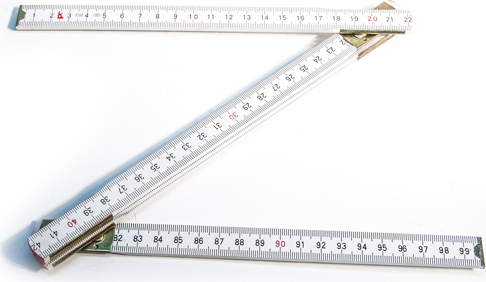
\includegraphics[scale=0.3]{meter.png}
%\end{center}
%\label{meter}
%\end{figure}
\end{minipage}
\end{tabular}
\begin{enumerate}\setcounter{enumi}{7}
\item С помощью этой же линейки нетрудно продемонстрировать, что композиция откладываний
\begin{itemize}
\item \textbf{ассоциативна}, т.е. одни и те же манипуляции с линейкой мы можем производить в разном порядке, например, сначала разложить два ее начальных колена, а затем разложить два колена в конце, и это будет ровно то же самое, как в случае раскладывания сначала конечного участка, а затем начального --- финальная конфигурация линейки будет одинаковой;
\item \textbf{коммутативна}, т.е. можно взять две линейки, произвести над ними какие-то манипуляции по складыванию/раскладыванию, затем их состыковать, и результат (направление и число колен линейки от начальной точки до конечной) не будет зависеть от того, в каком порядке линейки будут состыкованы.
\end{itemize}
\item Кроме того, очевидно, что у каждого откладывания существует обратное, приводящее в результате к нулевому откладыванию. Для этого нужно произвести ровно ту же самую серию откладываний, только поменять направление. Или, что то же самое, пройти по линейке в обратную сторону.
\item Далее любое откладывание будем записывать буквами $a,b,c,\dots$, имея ввиду под ними как прибавления, так и вычитания.
\item Откладывание, противоположное $a$, будем обозначать $-a$. При этом комбинация откладываний соединяется знаком '+', а если встречается комбинация $a+(-b)$, то пишем проще: $a-b$.
\item Обратные откладывания --- это просто перевернутые в обратную сторону <<линейки>>!
\item Результат откладывания (конфигурацию линейки с учтом ее направления) будем называть \textbf{вектором}. Если вектор смотрит влево (финишная точка левее стартовой), то вектор называется \textit{отрицательным}, а если вправо --- \textit{положительным}. Нулевой вектор --- когда финиш и старт совпадают.
\item Композицию откладываний будем называть \textbf{суммой векторов} или просто суммой, а процедуру откладывания --- \textbf{сложением}.
\end{enumerate}

\textbf{Свойства сложения}:
\begin{enumerate}[label=S\arabic*]
\item $(a+b)+c=a+(b+c)$ (ассоциативность).\index{Ассоциативность}
\item $a+b=b+a$ (коммутативность).\index{Коммутативность}
\item $a+0=0+a=a$ (аддитивное свойство нуля).\index{Нейтральный элемент}

Первые 3 свойства выше уже были продемонстрированы в процессе определения операций с линейкой. Добавим, что откладывания линейки еще можно рассматривать как путь некоего одномерного путешественника, который идет по прямой линии то вправо, то влево. Если он идет вправо, то прибавляет шаги, а если влево, то вычитает, т.е. делает обратный отсчет. Нулевой путь означает, что он прошел в одну сторону столько же, сколько в другую.

\item $a+(-a)=0$ (обратный элемент).\index{Обратный элемент}

Здесь помогает та же иллюстрация с путешественником. Он прошел сначала вправо $a$ шагов, затем влево столько же. В итоге пришел в начало пути, а это и означает по определению, что он прошел нулевой путь.

Конечно, с точки зрения физики он прошел в два раза больше, чем в одну сторону, но нас в данном случае интересует не то, сколько он потратил времени или сил на проделанный маршрут, а то, в какой точке линейки он оказался в финале. Для измерения его физических потерь нам потребуется ввести понятие пути и его длины. Но это мы отложим до более глубоких изысканий.

\item Если $a+x=b+x$, то $a=b$ (правило сокращения).

Добавим к исходному равенству в обоих частях элемент $-x$, обратный к $x$, и получим
$$
(a+x)+(-x) = a+(x+(-x)) = a,
$$
где мы воспользовались ассоциативностью операции сложения. Аналогично заключаем, что $(b+x)+(-x) = b+(x+(-x)) = b$. Таким образом, $a=b$.

\item Верно одно и только одно: либо $a=b$, либо $a=b+x$, либо $a=b-x$, где $x$ --- откладывание вправо (трихотомия).

Это утверждение также требует наглядного интуитивного доказательства. Тут нужно понимать, что наша линейка представляет собой один связный отрезок, а значит, путешественник может пройти по ней из любой точки в любую точку. Отметим на ней две точки $a$ и $b$. Если $a$ находится левее $b$, то нужно пройти положительный путь от $a$ к $b$, это и есть наше $x$, а если наоборот, то отрицательный, т.е. $-x$.
\end{enumerate}

\begin{enumerate}\setcounter{enumi}{14}
\item Понятие отрицательного и положительного векторов позволяют ввести сравнение на векторах.
\item Для начала скажем, что положительный вектор больше нуля: $x>0$.
\item Далее, если $b=a+x$, где $x>0$, то пишем $a<b$.
\item \textbf{Свойства сравнения} (очевидны):
\begin{enumerate}[label=O\arabic*]
\item не верно, что $x<x$ (антирефлексивность);
\item если $a<b$ и $b<c$, то $a<c$ (транзитивность);
\item верно одно и только одно: либо $a=b$, либо $a<b$, либо $b<a$ (трихотомия);
\item $a<b\Leftrightarrow a+x<b+x$, где $x>0$ (изотропность сравнения)
\end{enumerate}

\end{enumerate}


\lesson{Визуализация умножения через площадь и объем}


\begin{enumerate}
\item Строим две перпендикулярно направленные оси $Ox$ и $Oy$. На каждой оси --- свой собственный мир векторов и линеек.
\item Умножение --- это площадь, построенная на перпендикулярных векторах. Картинка $5\times 3=15$ (см. рис. \ref{prod}).
\begin{figure}[hbt!]
\begin{center}
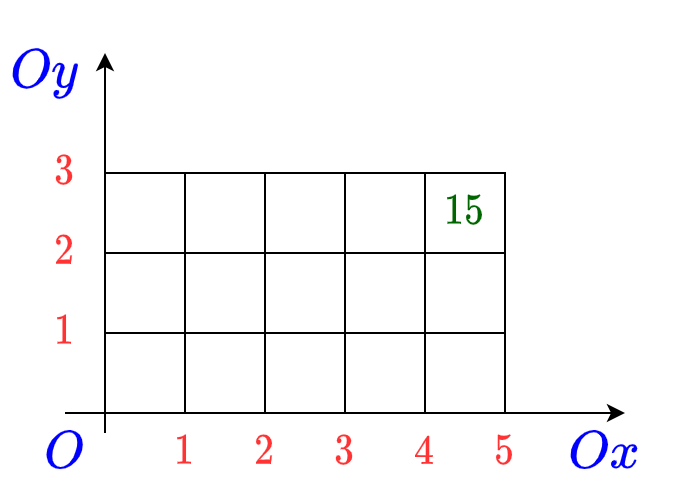
\includegraphics[scale=0.2]{prod.png}
\end{center}
\caption{}\label{prod}
\end{figure}
\item Площадь --- величина всегда положительная, а векторы мы умеем откладывать вверх и вниз, вправо и влево, т.к. имеем две перпендикулярные линейки. Соответственно, у нас имеется 4 различных ситуации: вправо и вверх, вправо и вниз, влево и вверх, влево и вниз.

Здесь мы впервые сталкиваемся с таким понятием, как \textit{ориентированная площадь}. Представим себе, что в нашу плоскость воткнута перпендикулярная ось, с конца которой мы наблюдаем за откладыванием векторов и подсчетом площадей. Когда первый вектор отложен вправо, а второй вверх, то площадь прямоугольника, наблюдаемая нами сверху, заметается по направлению от первого вектора ко второму. Такое направление (против часовой стрелки, или от оси $Ox$ к оси $Oy$) в математике принято считать положительным направлением. Поэтому соответствующую площадь мы считаем положительной.\footnote{То, что именно такое направление следует называть положительным, --- это всего лишь вопрос договоренностей о теримнах.}

\begin{figure}[hbt!]
\begin{center}
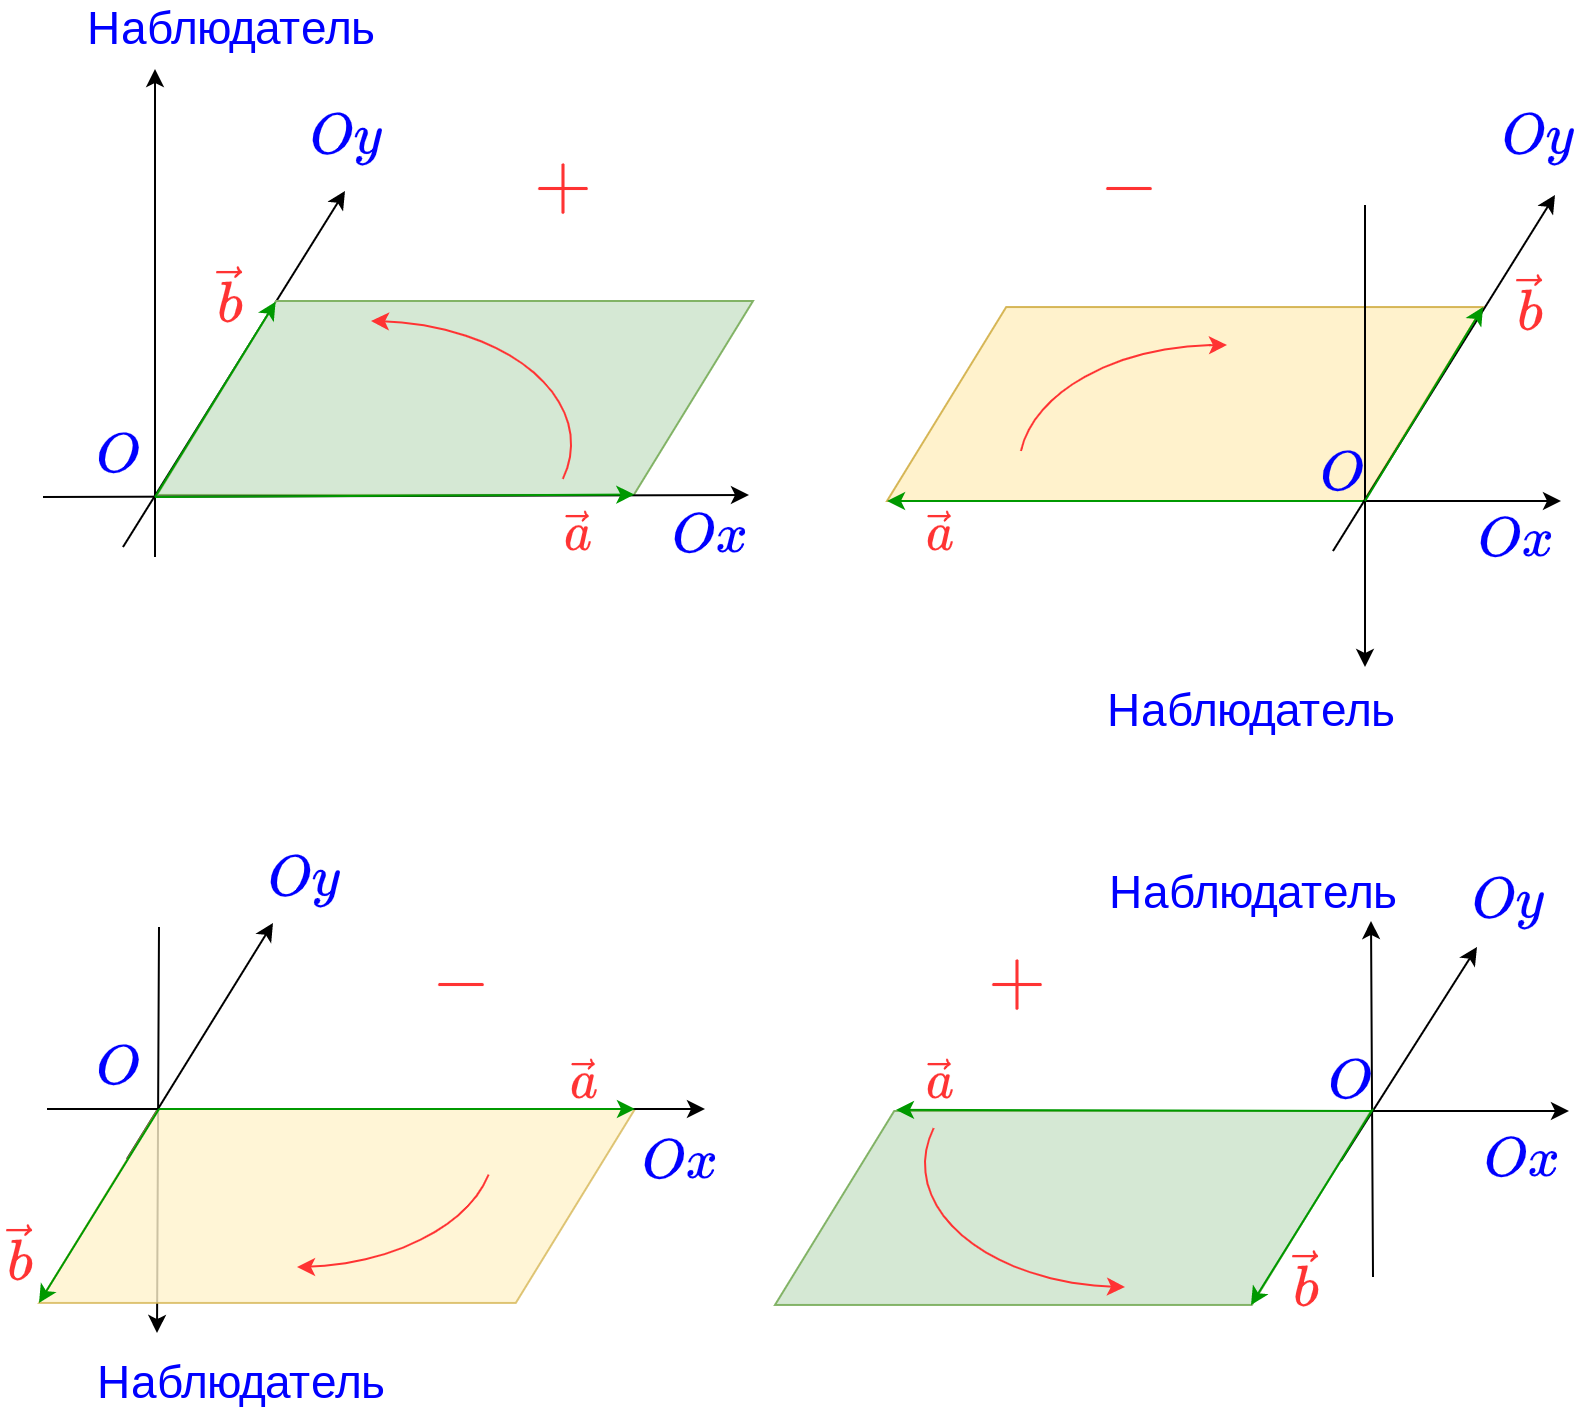
\includegraphics[scale=0.2]{mult.png}
\end{center}
\caption{}\label{mult}
\end{figure}

Теперь перевернем правый вектор, лежащий на оси $Ox$ и смотрящий вправо, через начало координат, в результате чего он будет смотреть влево и станет отрицательным. Вместе с ним перевернется и наш прямоугольник, площадь которого мы наблюдаем. И вместе с ним перевернется и наблюдательная вышка. Ее направление станет противоположным. И хотя мы по-прежнему с ее конца будем наблюдать площадь в правильном направлении, вся конструкция перевернется и сменит ориентацию в пространстве на противоположную, поэтому произведение отрицательного вектора на положительный станет также отрицательным.

Далее мы перекинем вектор, лежащий на оси $Oy$ через начало координат, так что он станет смотреть вниз, и прямоугольник. построенный на этих векторах, снова окажется в правильном, положительном положении, хотя обе его стороны есть отрицатлеьные числа. Стало быть, произведение двух отрицателных чисел есть число положительное.

Наконец, еще одна манипуляция с вектором $Ox$ в обратную сторону снова переведет конструкцию в отрицательное положение, и произведение снова станет отрицательным.

Итак, мы видим, что как только мы снабжаем плоскость дополнительным пространственным ориентиром, мы можем различать знак площади, сделать ее ориентированной в зависимости от того, куда направлены векторы, порождающие данную площадь.

В дальнейшем мы столкнемся с еще болеее общей конструкцией, где будем строить ориентированную площадь на произвольном параллелограмме. Но и там ситуация распадется на два знаковых класса в зависимости от ориентации векторов.

Таким образом, знак умножения двух чисел (площадь) определяется знаком (направлением) векторов и таблицей композиции знаков:
\begin{center}
\begin{tabular}{c|c|c|}
  & $+$ & $-$ \\
 \hline
$+$ & $+$ & $-$ \\
 \hline
$-$ & $-$ & $+$ \\
\hline
\end{tabular}
\end{center}
\item Данная таблица демонстрирует нам простейший пример группы. Во-первых, мы видим здесь, что композиция знаков тоже есть знак, во-вторых, что композиция любого знака с плюсом ничего не меняет, т.е. плюс является нейтральным в операции композиции. В-третьих, что знак минус сам себе обратен, так как умножение его самого на себя дает плюс. Все эти свойства являются определяющими свойствами математического понятия группы, и будут <<работать>> на потяжении всгео курса.


\item Отметим, что умножение можно иллюстрировать не только площадью, но и объемом, если нам необходимо перемножить три числа. Хотя сама по себе операция умножения бинарная (т.е. имеет два аргумента), один из множителей, в свою очередь, также может быть результатом операции умножения, так что в итоге получается умножение трех чисел. Более того, любое число $a$ можно представить как площадь прямоугольника $a\times 1$. И наоборот, произведение $a\times b$ можно вытянуть в линию из $ab$ квадратиков, тем самым перейдя от площали к отрезку. Поэтому в дальнейшем умножение векторов в смысле нахождения площади/объема, т.е. $a\times b$, и умножение чисел как таковых, т.е. $ab$, будем считать одним и тем же понятием и обозначать одинаково, так что $a\times b=ab$.

\item \textit{Степень}: многократное умножение отрезка самого на себя. Поскольку степень есть частный случай многократного умножения, то вотрая степень, очевидно, представляется площадью квадрата, третья --- куба, а для иллюстрации более высоких степеней потребуются и более высокие размерности.
\end{enumerate}


\textbf{Свойства умножения}:
\begin{enumerate}[label=P\arabic*]
\item $(a\times b)\times c = a\times (b\times c)$ (ассоциативность --- рис. \ref{assoc});\index{Ассоциативность}

\begin{figure}[hbt!]
\begin{center}
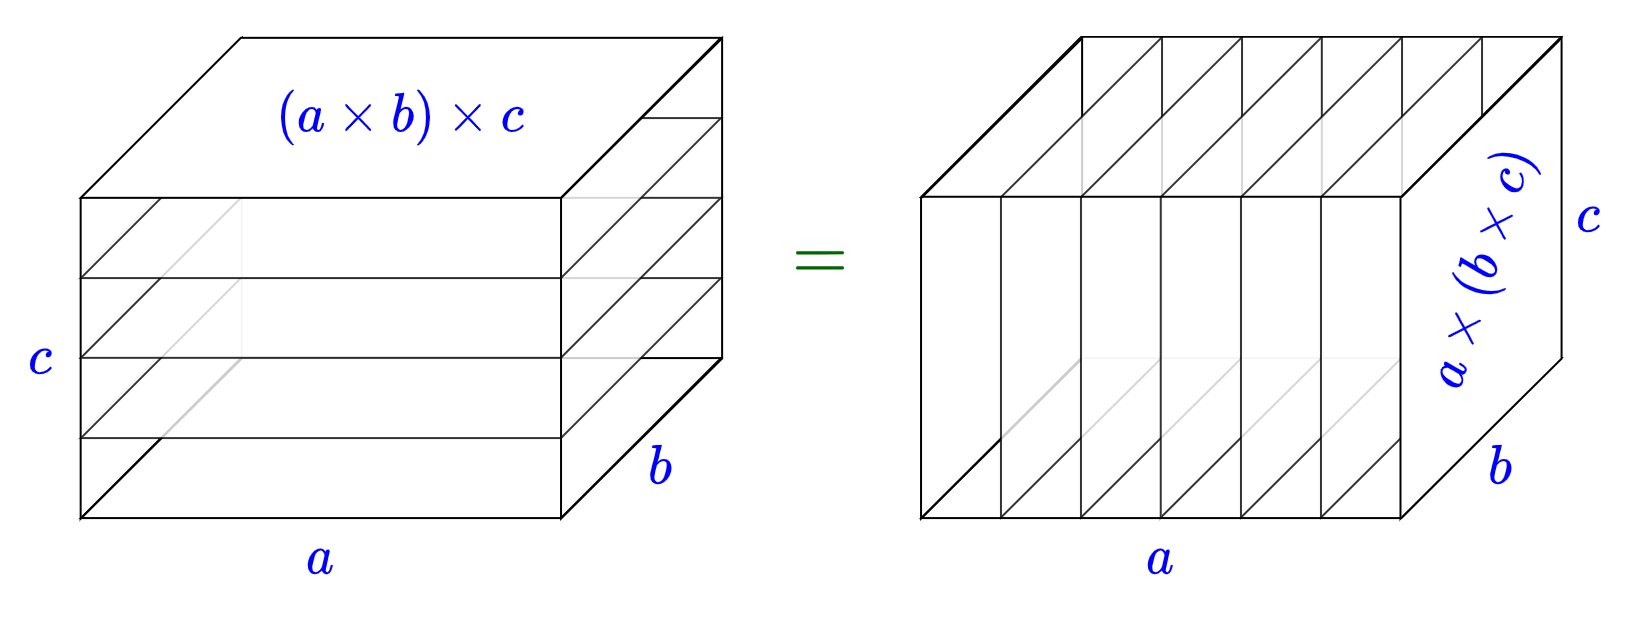
\includegraphics[scale=0.2]{assoc.png}
\end{center}
\caption{}\label{assoc}
\end{figure}

\item $a\times b=b\times a$ (коммутативность --- рис. \ref{kommut});\index{Коммутативность}

\begin{figure}[hbt!]
\begin{center}
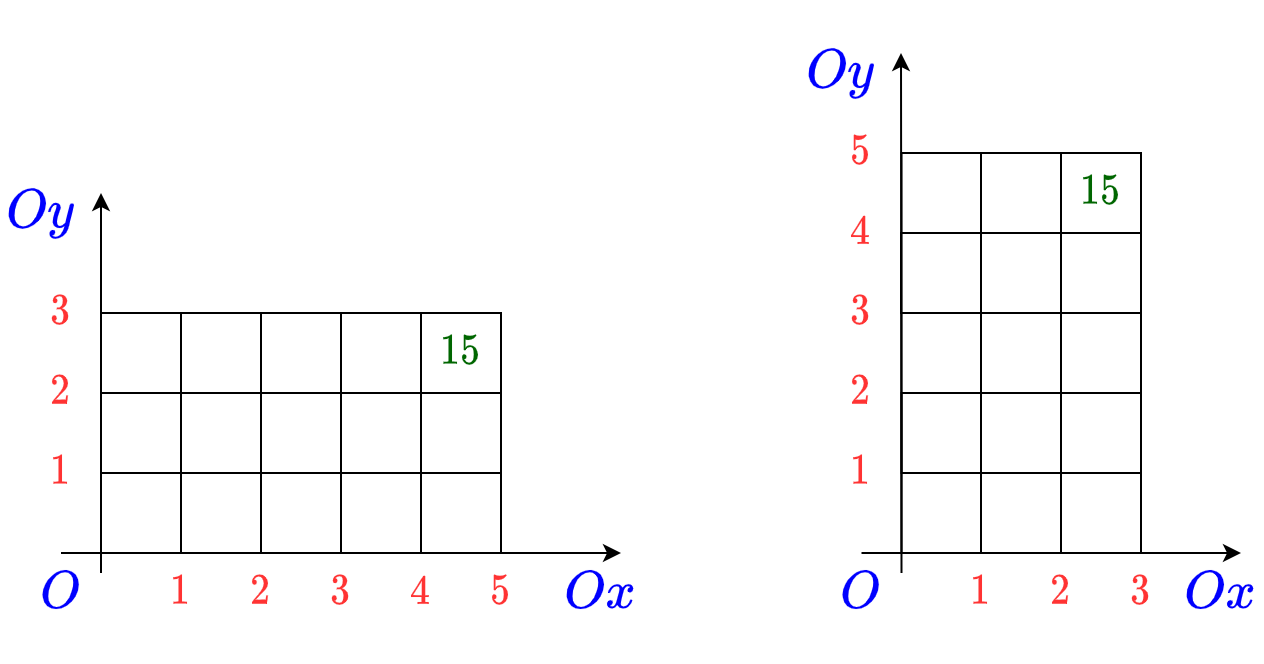
\includegraphics[scale=0.2]{kommut.png}
\end{center}
\caption{}\label{kommut}
\end{figure}

\item $a\times 1=1\times a=a$ (нейтральный элемент по умножению);\index{Нейтральный элемент}

\item $a\times(b+c)=a\times b+a\times c$ (дистрибутивный закон --- рис. \ref{distr});\index{Дистрибутивность}

\begin{figure}[hbt!]
\begin{center}
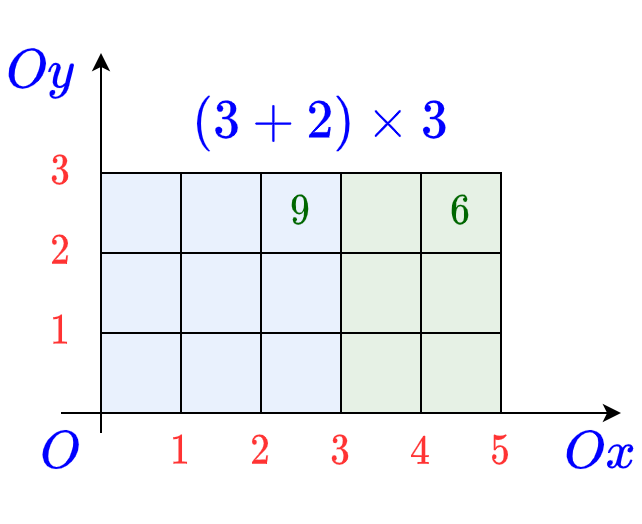
\includegraphics[scale=0.2]{distr.png}
\end{center}
\caption{}\label{distr}
\end{figure}

\item Умножение на нулевой отрезок (мультипликативное свойство нуля) --- применим свойство сложения с нулем, дистрибутивность и сокращение на одинаковое слагаемое:\index{Мультипликативное свойство нуля}
$$
0 + a\times 0 = a\times 0 = a\times (0+0) = (a\times 0) + (a\times 0)\Rightarrow 0 = (a\times 0).
$$

\item если $a\times b=0$, то $a=0$ или $b=0$ (отсутствие делителей нуля);\index{Делители нуля}

Предполагая, что $a\ne0\ne b$, построим прямоугольник $a\times b$, он точно будет ненулевой площади --- см. рис. \ref{prod}.

\item если $a\times c=b\times c$ и $c\ne 0$, то $a=b$ (правило сокращения);

Найдем разность и воспользуемся дистрибутивностью:
$$
0 = a\times c-b\times c = (a-b)\times c,
$$
а так как $c\ne 0$, получаем, что $a-b=0$, т.е. $a=b$.

\item если $a<b$ и $c>0$, то $a\times c<b\times c$, и обратно: если $a\times c<b\times c$ и $c>0$, то $a<b$ (монотонность --- рис. \ref{monot});

\begin{figure}[hbt!]
\begin{center}
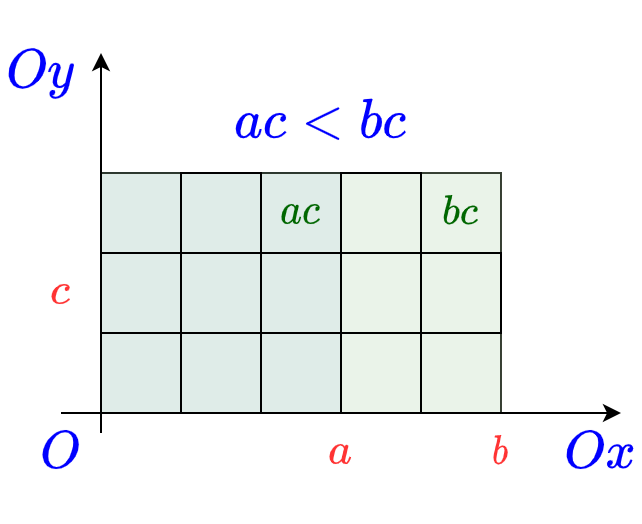
\includegraphics[scale=0.2]{monot.png}
\end{center}
\caption{}\label{monot}
\end{figure}

\end{enumerate}


\subsection*{Задачи}
\begin{enumerate}
\item Нанести метки на прямой, соответствующие шагам вправо и влево, считая начальной точкой $O$, а все шаги равновеликими. Дойти до точки 10 и -10.
\item Описать в терминах одномерного путешественника операции сложения: $5+3$, $8-4$, $3-5$, $-2-6$.
\end{enumerate}



\section{Понятие натурального числа}

\lesson{Натуральные числа как кратность операций сложения и умножения. Понятие делимости/кратности. Ноль кратен любому числу}

\begin{enumerate}
\item Ранее мы вводили определение степени числа как многократного применения операции умножения на одно и то же число. Ясно, что то же самое можно определить и в отношении многократной операции сложения одного и того же числа с самим собой. Только в случае сложения <<степень>> есть обычное умножение. Действительно, многократное сложение $a+a+a+a+a+\dots$, если воспользоваться графическим представлением, есть просто умножение отрезка $a$ на отрезок длины $1+1+1+\dots$, где единицы взяты ровно в том же количестве, в каком встречается $a$ (рис. \ref{kratplus}).

\begin{figure}[hbt!]
\begin{center}
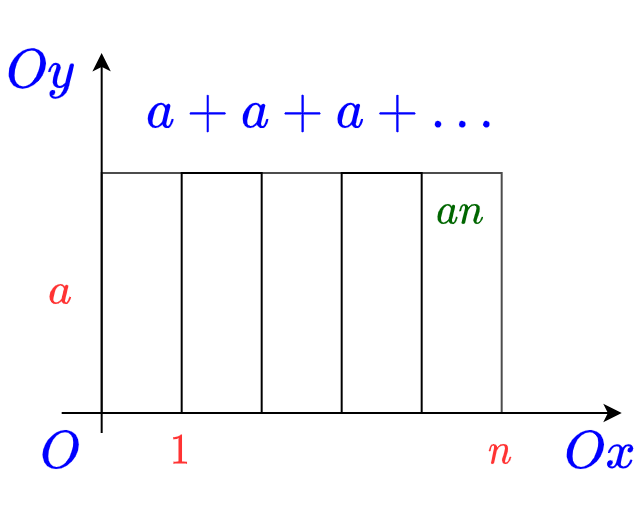
\includegraphics[scale=0.2]{kratplus.png}
\end{center}
\caption{}\label{kratplus}
\end{figure}

В итоге, если мы число $a$ складываем $n$ раз (где $n$ --- это обозначение суммы единиц), то это все равно, что мы производим умножение
$$
a\times(\underbrace{1+1+\dots+1}_{n}).
$$

В случае многократного умножения действуем по аналогии:  $a a a\ldots$ обозначаем как $a^n$, понимая под $n$ количество чисел $a$, которые мы перемножили.

Вот эта количественная роль чисел, которые выступают для обозначения кратности однотипных операций, и является смыслом натурального числа. Натуральное число есть ответ на вопрос <<сколько раз?>> или <<сколько штук?>>

Целые числа не могут похвастаться таким натуральным (предметным) определением. В целых числах к количеству добавляется еще и направление (назад или вперед, но об этом --- позже), а рациональное число отражает отношение между количествами.

\item Нулевая кратность: в случае сложения ничего не складываем, остаемся на месте в начальной точке, поэтому
$$
\underbrace{a+\dots+a}_{0\mbox{ раз}}=0.
$$
\item Нулевая степень: в случае умножения ничего не умножаем, от умножения остается только 1:
$$
\underbrace{a\times\dots\times a}_{0\mbox{ раз}}=1.
$$
Почему именно 1? Потому что если мы начнем перемножать разные числа с разными кратностями
$$
\underbrace{aa}_{?}\underbrace{bbbb}_{?}\underbrace{ccccc}_{?},
$$
то результат не должен меняться, если кратность одной из переменных станет равной нулю. В данном примере любую из кратностей можно сделать нулевой, тогда эта переменная выпадет из записи, и результат останется верным, только если нулевая кратность умножения равна 1.

Многие правила в математике для крайних значений определяются с целью сохранить общий вид формул, если это не приводит к противоречию.
\item Итак, \textbf{натуральные числа}\index{Числа!натуральные}\index{Натуральные числа} --- это показатели кратности операций (сложения и умножения).
\item С другой стороны, ничто не мешает нам сумму единиц рассматривать саму по себе, т.е. как сумму единичных отрезков. В данном случае нет никакой разницы между суммой единичных отрезков и кратностью сложения единичного отрезка.
\item Такая интерпретация натурального числа вполне согласуется с операциями сложения и умножения, сохраняет все законы арифметики: ассоциативность, коммутативность, дистрибутивность.
\item Поэтому натуральные числа, привязанные к единичным отрезкам, можно также считать мерой длины, площади, объема и т.д.
\item Ноль мы будем считать натуральным числом, поскольку мы рассматриваем нулевую кратность для однородности законов арифметики.
\item[\bf NB] Натуральные числа --- это и кратности операций, и единицы измерения, т.е. числа.
\item Натуральные числа отвечают за соизмеримость и арифметическую кратность чисел (любых): $a$ \textbf{кратно}\index{Кратность чисел} $b$ ($a\mathop{\vdots} b$), если $a=bn$ или $a=(-b)n$ при некотором натуральном $n$. Ноль кратен любому числу! Нулю кратен только ноль!

Действительно, $0\mathop{\vdots} b$ означает, что при некотором $n$ имеем $0=bn$. Это верно как раз при $n=0$. Предположим, что какое-то число кратно нулю: $a\mathop{\vdots} 0$, тогда при некотором $n$ должно быть $a=0n$. Но при любом $n$ имеем $0n=0$, так что только $a=0$ будет кратно нулю.

\item Если $a$ кратно $b$, то говорят также, что $b$ \textbf{делит} $a$, или что $b$ является делителем $a$ ($b|a$).\index{Делимость чисел}
\item Если $a>0$ кратно $b>0$, то $a=kb=b+(k-1)b$, где $k>0$. Здесь $x=(k-1)b$. Поэтому $a\ge b$. Так что для положительных векторов кратность означает превосходство в смысле сравнения. Аналогичные неравенства можно получить и для отрицательных векторов.
\end{enumerate}
\subsection*{Задачи}
\begin{enumerate}
\item Доказать, что если $a|b$ и $b|c$, то $a|c$.
\item Доказать, что если $a|b$ и $b|a$, то $a=\pm b$ ($a,b$ --- произвольные векторы).
\end{enumerate}


\section{Визуальные доказательства}

\lesson{Теорема Пифагора геометрически. Бином Ньютона разрезанием кубика}
\href{https://www.youtube.com/watch?v=Xdc8WWFURA8}{Видеоурок про теорему Пифагора}

\href{https://www.youtube.com/watch?v=YXYQmxLDtMw}{Видеоурок про бином Ньютона}

\begin{enumerate}
\item \textbf{Квадрат суммы}. Строим квадрат $(a+b)\times (a+b)$ и внутри него квадраты $a\times a$ и $b\times b$ (см. рис. \ref{pithagor}). Приравнивая площадь всего квадрата к сумме его частей, получаем, что
$$
(a+b)^2 = a^2 + 2ab + b^2.
$$
\item \textbf{Теорема Пифагора}. Далее, строим еще один квдарат $(a+b)\times (a+b)$ и внутри квадрат $c\times c$, где $c$ --- это гипотенуза треугольника с катетами $a$ и $b$ (рис. \ref{pithagor}). Далее заштрихуем одинаковые треугольники в левом и правом квадратах. А поскольку оба больших квадрата равны, равны и их площади, а также площади тех остатков, которые получается, если выбросить заштрихованные треугольники. То, что остается, дает равенство:
$$
a^2+b^2=c^2,
$$
т.е. теорему Пифагора.

\begin{figure}[hbt!]
\begin{center}
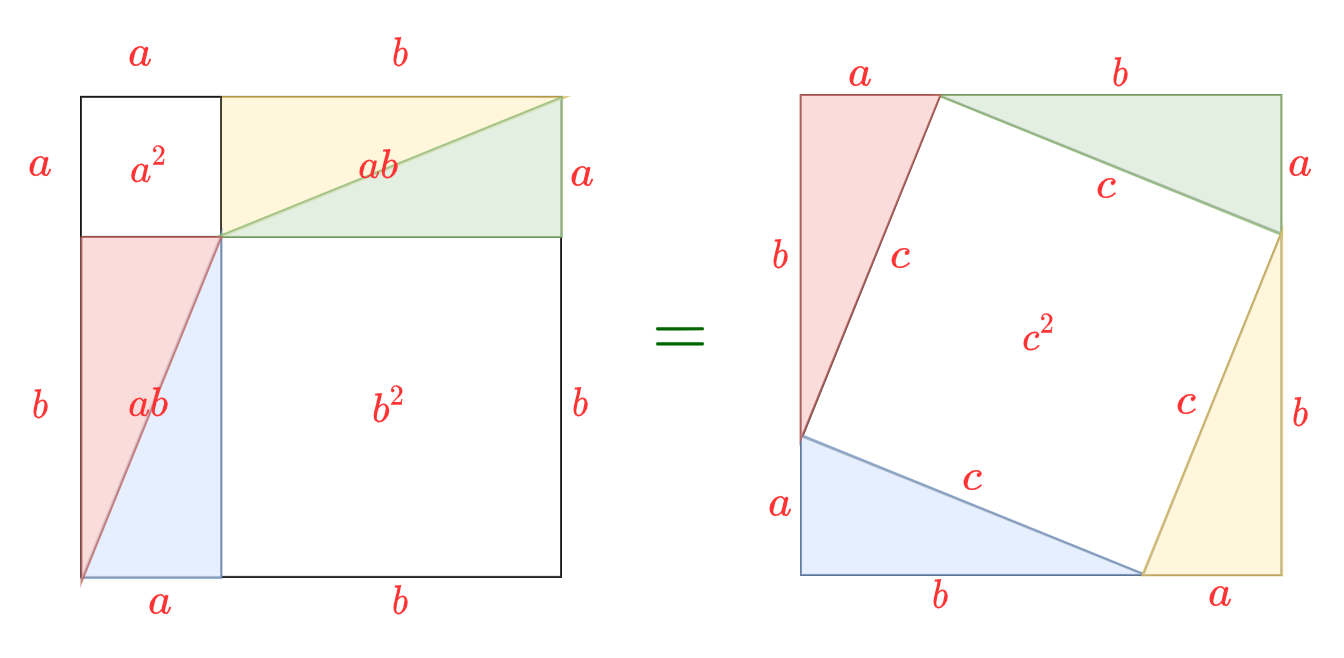
\includegraphics[scale=0.25]{pithagor.png}
\end{center}
\caption{}\label{pithagor}
\end{figure}

\item \textbf{Разность квадратов}. Визуализация $(a-b)(a+b)=a^2-b^2$ (рис. \ref{razn}).
\begin{figure}[hbt!]
\begin{center}
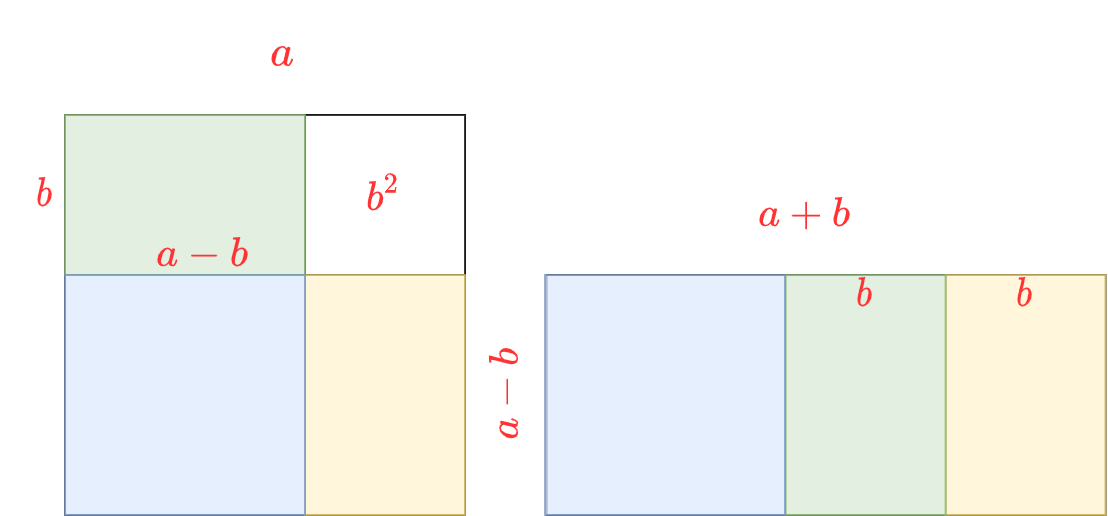
\includegraphics[scale=0.25]{razn.png}
\end{center}
\caption{}\label{razn}
\end{figure}

\item \textbf{Сумма подряд идущих чисел} $1,2,\dots,n$. Решаем для случая четного $n$.
Расставляем прямоугольники $1\times k$ лесенкой от самого маленького к самому большому (рис. \ref{ariphm}). Далее замечаем, что если последний переложить на первый, предпоследний на второй, и т.д., то будут получаться одинаковые прямоугольники высотой $n+1$. Получится $n/2$ прямоугольников длины $n+1$, так что сумма равна $n(n+1)/2$.

\begin{figure}[hbt!]
\begin{center}
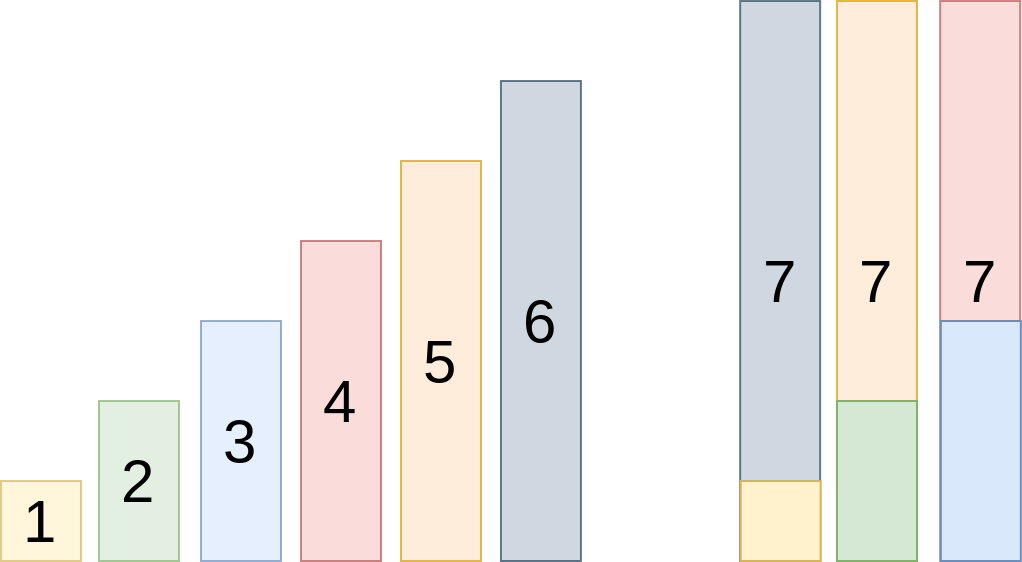
\includegraphics[scale=0.2]{ariphm.png}
\end{center}
\caption{}\label{ariphm}
\end{figure}

Если $n$ --- нечетное, то применим тот же метод, отставив в сторону последнее слагаемое $n$. Получится $(n-1)/2$ столбиков высотой $n$ и плюс еще один столбик высотой $n$. Итого, снова будем иметь сумму $n(n+1)/2$

\item \textbf{Бинома Ньютона для} $n=3$: $(a+b)^3 = a^3+3a^2b+3ab^2+b^3$. Разрезание сырного кубика на 8 частей тремя плоскостями. См. рис. \ref{kub}

\begin{figure}[hbt!]
\begin{center}
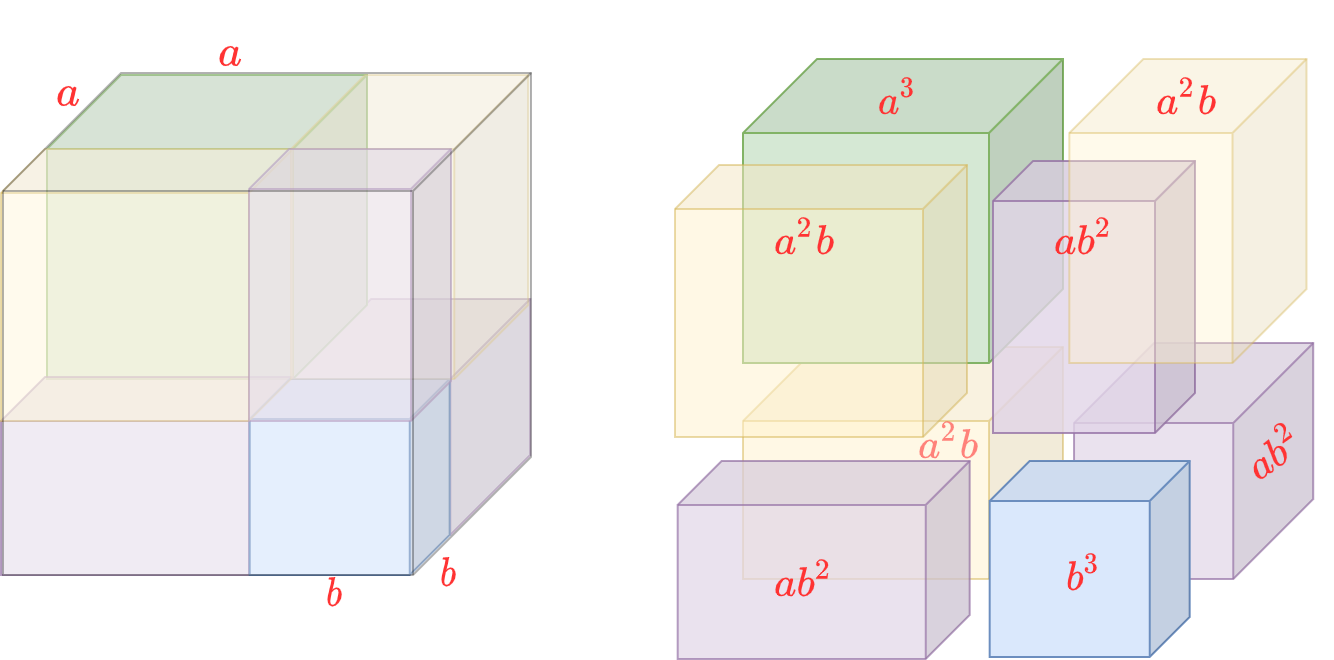
\includegraphics[scale=0.25]{kub.png}
\end{center}
\caption{}\label{kub}
\end{figure}
\end{enumerate}

\subsection*{Задачи}

\begin{enumerate}
\item Найти с помощью графического метода сумму подряд идущих нечетных чисел от 1 до $n$, где $n$ --- нечетное.
\end{enumerate}


\section{Соизмеримость отрезков, алгоритм Евклида}


\lesson{Соизмеримость отрезков. Кузнечики и визуальный алгоритм Евклида}

\begin{enumerate}
\item Пусть у нас на числовой прямой сидят в точке $O$ два кузнечика. Один умеет прыгать на длину $a$ как вправо, так и влево, а второй --- на длину $b$ как вправо, так и влево.

\item Могут ли они через какое-то конечное количество прыжков попасть в одну и ту же точку, отличную от $O$?
\item Ответ --- да, если есть такая точка $A$, что отрезок $OA$ кратен и $a$, и $b$ одновременно, т.е. при некотрых натуральных $n,m$, не равных нулю, будет верно равенство $an=bm$:
$$
\underbrace{a+a+\dots+a}_{n\mbox{ раз}}=\underbrace{b+b+\dots+b}_{m\mbox{ раз}}
$$
\item Отрезки, которые имеют общий кратный отрезок, называются \textbf{соизмеримыми}.\index{Соизмеримость}
\item Из равенства $an=bm$ видно, что есть общий отрезок $c=a/m=b/n$, который целое число раз укладывается как в $a$, так и в $b$. Такой отрезок $c$ называется \textbf{наибольшим общим делителем} $a$ и $b$ и обозначается $\gcd(a,b)$. Ясно, что он существует тогда и только тогда, когда существует отрезок $OA$, кратный отрезкам $a$ и $b$.

Действительно, если $c=\gcd(a,b)$ существует, то он, являясь делителем, имеет представление $c=a/m=b/n$ при некоторых положительных натуральных $n,m$, откуда $an=bm$, и отрезок $OA$ длины $an$ является искомым. Обратно, если существует отрезок $OA$, одновременно кратный как $a$, так и $b$, то имеет место представление $OA=an=bm$, откуда число $c=a/m=b/n$ является делителем как $a$, так и $b$, а значит, их общим делителем, следовательно, существует и $\gcd(a,b)$.

\item На этот отрезок можно выйти другим путем: строим прямоугольник $a\times b$ ($a<b$), начинаем отсекать в нем квадраты: сначала отсекаем квадраты $a\times a$, пока можем, останется кусок $a\times b_1$ ($b_1<a$), затем отсекаем квадраты $b_1\times b_1$, пока можем, останется кусок $a_1\times b_1$ ($a_1<b_1$), и т.д.
\begin{figure}[hbt!]
\begin{center}
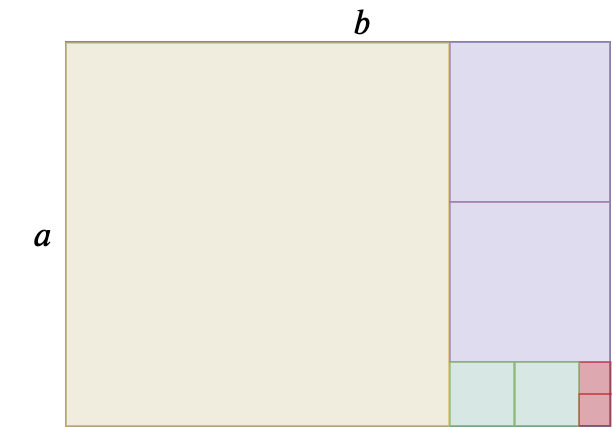
\includegraphics[scale=0.3]{soizmer.png}
\end{center}
\caption{}\label{soizmer}
\end{figure}

\item Если исходные отрезки соизмеримы, то процесс остановится: исходный прямоугольник будет разбит на конечное число квадратиков. При этом можно заметить, что самые мелкие квадратики целое число раз укладываются во все более крупные просто по построению. Это значит, что прямоугольник $a\times b$ можно разбить на конечное число маленьких квадратиков, общее число которых будет $nm$ штук.

Действительно, соизмеримость $a$ и $b$ означает, что стороны прямоугольника можно разбить на целое число частей длины $c=a/m=b/n$, а процесс разрезания этого прямоугольника на квадраты всегда будет происходить по сетке с шагом $c$, причем каждый раз шаг разрезания будет уменьшаться. Но у нас конечное число квадратиков $c\times c$, стало быть, процесс разрезания рано или поздно упрется в прямоугольник со стороной $c$, который уже будет разделен на целое число квадратов. На этом алгоритм и закончится.

\item Длина стороны финального квадратика будет иллюстрировать НОД отрезков $a$ и $b$, т.к. это максимальный квадрат, которым можно замостить прямоугольник $a\times b$. 

Действительно, любой квадрат, которым можно замостить прямоугольник $a\times b$, целое число раз укладывается в квадрат $a\times a$ и, как следствие, в оставшийся прямоугольник $a\times(b-a)$, а значит, целое число раз укладывается в квадрат $(b-a)\times (b-a)$ и, как следствие, в оставшийся прямоугольник, и т.д. То есть, если каким-то квадратом можно замостить исходный прямоугольник, то им же можно замостить и финальный маленький квадратик. Следовательно, этот квадратик наибольший из всех таких. которыми можно замостить прямоугольник $a\times b$.
\item Такой процесс постепенного спуска к НОД называется \textbf{алгоритмом Евклида},\index{Алгоритм Евклида} к нему мы еще неоднократно вернемся с более формальной точки зрения.
\item Заметим, что числа $a$ и $b$ при этом вовсе не обязаны быть натуральными. Это --- какие-то векторы на числовой прямой. в том числе они могут быть отрицательными (при этом их НОД, если он существует, всегда выбирается со знаком плюс).
\end{enumerate}
\subsection*{Задачи}
\begin{enumerate}
\item Найти НОД(10,6) методом прямоугольников.
\item Сколько и каких шагов должны сделать 10- и 6-шаговые кузнечики, чтобы попасть в точку НОД(10,6)?
\end{enumerate}



\newchapter{Движения прямой}

\vrezka{В этой главе мы переходим к более формальной работе с точками и векторами на прямой. Целью является знакомство с понятиями <<движение>>, <<композиция движений>>. Проводится полный анализ видов движений и свойств их композиций.

Попутно вводится понятие группы и подгруппы в приложении к группе движений на прямой. Изучаются все конечные подгруппы движений прямой.\index{Движения!прямой}
}

\section{Сдвиг, композиция сдвигов, группа}

\lesson{Иллюстрация сдвигов с помощью линейной парковки. Обозначения сдвигов. Композиция сдвигов. $\id$ и обратный сдвиг. Фрмулировка аксиом группы}


\begin{enumerate}
\item \textbf{Иллюстративная сказка}. Представим себе очень длинную однорядную автомобильную парковку на территории какого-нибудь бизнес-центра. На этой парковке размечены места номерами 0, 1, 2 и т.д. (слева направо). В какой-то момент парковку достроили влево и решили, не мудрствуя лукаво, продолжить нумерацию отрицательными числами $-1$, $-2$, $-3$ и т.д. Получилась шкала примерно как на градуснике для измерения уличной температуры. Водителям, работающим в этом бизнес-центре, выдали парковочные талоны с номерами парковочных мест, т.е. такие же числа 0, $\pm 1$, $\pm 2$ и т.д. В соответствии с талонами они занимают свои места, так что получается, что водитель с талоном номер 0 встает на место номер 0, водитель с талоном номер 1 --- на место номер 1 и т.д.
\item Но потом появляется необходимость поменять бордюр и плитку там, где находятся два крайних левых парковочных места, пусть это будут номера $-3$ и $-2$. Возникает потребность куда-то девать те а/м, для которых зарезервированы номера $-3$ и $-2$. Вместо того, чтобы предложить обменять талоны $-3$ и $-2$ на резервные номера парковки, начальнику охраны приходит в голову гениальная идея: повесить на въезде плакат с надписью (красным фломастером на А4): <<Внимание! Занимайте номер парковки на 2 больше, чем указан в вашем талоне!!>>
\item Так что водитель, имеющий парковочный талон номер -3, занимает место -1, номер -2 --- место 0, номер -1 --- место 1, и т.д.

\begin{figure}[hbt!]
\begin{center}
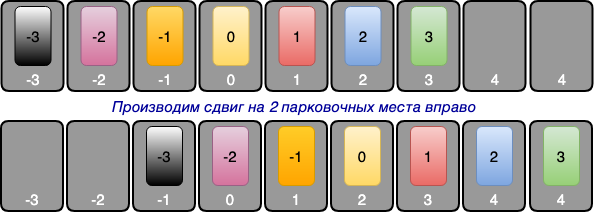
\includegraphics[scale=0.3]{TT.png}
\end{center}
\caption{}\label{TT}
\end{figure}
\item Иначе говоря, все автомобили должны теперь вставать на 2 места правее, т.е. произвести сдвиг относительно своего обычного места, указанного в парковочных талонах (см. рис. \ref{TT}).
\item Отметим еще одну особенность истории с парковкой: несмотря на произведенное перемещение автомобилей, они по-прежнему остаются на парковке, не занимая места где-либо еще, например, на проезжей части или тротуаре. Просто потому, что запас мест справа оказался достаточным для данной манипуляции.
\item А что, если бы парковка была неограниченно расширяемой в обе стороны автоматически всякий раз, когда не хватает места? Как говорят математики, она была бы потенциально бесконечной.
\item Геометрически мы можем представить это так: у нас имеется прямая, на которой нанесена разметка числами 0, $\pm 1$, $\pm 2$ и т.д. через равные расстояния между соседними точками. Прямая --- бесконечная в обе стороны. Но вдруг возникает необходимость сдвинуть эту прямую вправо на 2 единицы. Для этого всем точкам прямой дается команда сдвинуться на вектор длины 2 вправо.
\item Однако, чтобы сохранить историю этого сдвига и проверить его правильность, следует сдвигать не саму прямую, а ее копию. В итоге мы получаем прямую-оригинал и прямую-образ. Если уж быть совсем точными, то у нас возникает то, что в математике называется функцией, т.е. соответствие между оригинальными точками и их точками-образами на копии прямой.
\item Так мы видим не только новое положение точек, после сдвига, но и как оно соотносится с прежним их положением!
\item Понятно, что сдвигать геометрическую прямую, не выходя за ее пределы, можно только вправо или влево, причем на вектор произвольной длины, не обязательно на число 2 или 3, или им подобное. Тем более что цифровую разметку на прямую можно и вовсе не наносить.
\item Преобразование, состоящее в том, что все точки прямой сдвигаются на вектор $a$, называется \textbf{сдвигом} на вектор $a$. При этом, чтобы узнать, в какую точку (относительно исходной разметки) перейдет точка $A$, нужно от точки $A$ отложить вектор $a$, т.е. найти сумму $A+a$. Это будет некоторая точка $A'$ на этой же прямой.
\item Преобразование сдвига на вектор $a$ обозначим $T_a$, а его действие на точку $A$ обозначим $T_a(A)$. Так что
$$
T_a(A)=A',\quad a=\vec{AA'}.
$$
\item Сдвиг является движением (не случайно это однокоренные слова!).
\item Вообще, \textbf{движение --- это преобразование, сохраняющее расстояния}\index{Движение} (размеры и форму): если между точками $A$ и $B$ было расстояние $x$, то после преобразования движения расстояние между точками $A'$ и $B'$, в которые перешли исходные точки, тоже будет $x$, и так для любой пары точек! Для сдвига эот очевидно, поскольку ко всем точкам прибавляется один и тот же вектор.
\item Математическое движение --- это результат физического движения (есть только начальное и конечное состояние системы).
\item Сдвиг характерен тем, что он в качестве параметра имеет только вектор, т.е. величину и направление сдвига, но он никак не связан с исходной разметкой прямой!
\item Композиция сдвигов --- это их последовательное применение:
\begin{equation}\label{Tcomposition}
(T_b\circ T_a)(A)=T_b(T_a(A)).
\end{equation}
\item Композиция сдвигов соответствует сумме векторов: $T_b\circ T_a=T_{a+b}$.
\item Композиция сдвигов перестановочна в силу коммутативности сложения: $$T_b\circ T_a=T_a\circ T_b.$$
\item Композиция сдвигов ассоциативна, т.е. если мы имеем последовательность из трех и более сдвигов, то мы можем начать вычислять ее с любого места цепочки, постепенно сворачивая выражение, как с обычными числами:
$$
T_a\circ T_b\circ T_c = (T_a\circ T_b)\circ T_c = T_a\circ (T_b\circ T_c),
$$
т.е. сначала вычислить композицию последних и результат подставить в первую, либо же наоборот --- сначала вычислить первую, и ее применить к последней. Это правило можно тиражировать на цепочку композиций любой длины. Результат при этом будет один и тот же, совершенно так же, как если бы мы складывали подряд несколько чисел.
\item Кратность сдвига обозначается как степень
$$
\underbrace{T_a\circ\dots\circ T_a}_{n\mbox{ раз}}=T_a^n
$$
и соответствует кратности сложения или сдвигу на вектор, получаемый умножением исходного вектора на степень кратности: $T_a^n=T_{an}$.
\item Нулевой сдвиг $T_0=\id$ --- это \textbf{тождественное преобразование}, которое ничего не меняет.
\item Обратный сдвиг $T_a^{-1}$ --- это сдвиг на вектор $-a$, т.е. сдвиг в обратном направлении на ту же величину.
\item Нулевой сдвиг сам себе обратен.
\item Вообще, если есть какие-то два преобразования $u$ и $v$ и операция композиции $\circ$, то эти преобразования \textbf{взаимно обратны}, если $u\circ v=\id$ и $v\circ u=\id$, т.е. последовательное применение этих преобразований в любом порядке является тождественным преобразованием (сводится к ничего не деланию).
\item Обобщая свойства сдвигов, фиксируем понятие \textbf{группы}.\index{Группа} Это --- такое множество $G$ с заданной на нем одной бинарной операцией $\circ$, для которой выполняются аксиомы:
\begin{enumerate}[{\bf G}1)]
\item Результат групповой операции снова лежит в этом же множестве (например, композиция сдвигов есть сдвиг):
$$
u,v\in G \Rightarrow u\circ v\in G.
$$
\item Групповая операция \textbf{ассоциативна} (сочетательный закон): для любых элементов $u,v,w$ группы $G$\index{Ассоциативность}
$$
(u\circ v)\circ w = u\circ (v\circ w)
$$
(например, $(T_a\circ T_b)\circ T_c=T_a\circ(T_b\circ T_c)$.
\item Существует \textbf{нейтральный элемент} $\id$ такой, что для любого элемента $u$ имеет место равенство\index{Нейтральный элемент}
$$
u\circ\id = u = \id\circ u.
$$
\item Групповая операция \textbf{обратима}: для всякого элемента $u$ существует обратный ему элемент $v$ такой, что
$$
u\circ v=\id = v\circ u
$$
(например, обратный сдвиг --- это сдвиг в противоположную сторону:  $T_{a}^{-1}=T_{-a}$). Элемент $v$ в таком случае обозначается как $u^{-1}$ и называется \textbf{обратным} к элементу $u$.\index{Обратный элемент}
\end{enumerate}
\item Множество всех сдвигов образует группу относительно операции композиции!
\item Мало того, группа сдвигов \textbf{коммутативна}\index{Коммутативность} (абелева), т.е. для ее групповой операции выполняется переместительный закон:\index{Группа!абелева}
\begin{enumerate}[resume*]
\item $u\circ v=v\circ u$ для всех $u,v$ из группы $G$.
\end{enumerate}
\item Кратность обратного сдвига: $T_a^{-n}\rightleftharpoons (T_a^{-1})^n=T_{-a}^n=T_{-an}=(T_{an})^{-1}$.
\item Обратный сдвиг к композиции сдвигов: $(T_a\circ T_b)^{-1}=T_b\circ T_a$. Это легко следует из общего свойства группы:
$$
(u\circ v)^{-1} = v^{-1}\circ u^{-1},\mbox{ поскольку }(u\circ v)\circ(v^{-1}\circ u^{-1})=u\circ(v\circ v^{-1})\circ u=\id.
$$
\item На основе только одного сдвига $T_a$ можно построить подгруппу сдвигов
$$
\langle T_a\rangle = \{T_a^n, T_a^{-n}\mid n=0,1,2,\dots\}
$$
\item Эта подгруппа --- реализация целых чисел $\Z$, к которым мы еще вернемся позже.
\item Фиксируем понятие \textbf{подгруппы}.\index{Подгруппа} Это --- подмножество группы, на котором групповая операция удовлетворяет групповым аксиомам, т.е. подгруппа сама является группой с той же операцией, которая задана в группе.\label{Subgroup}

Подгруппу можно определить иначе: непустое подмножество $H\subseteq G$ группы $G$ называется подгруппой, если для любых $a,b\in H$ имеет место $a\circ b^{-1}\in H$.

Оба определения эквивалентны. Действительно, если $H$ удовлетворяет первому определению, т.е. само является группой, то требование $(a,b\in H)\to (a\circ b^{-1}\in H)$ выполняется по определению группы автоматически. Обратно, если данное требование выполнено, то, очевидно, что единица группы $G$ принадлежит $H$ ($a\circ a^{-1}\in H$), обратный элемент к элементу $b\in H$ также принадлежит $H$, т.к. $\id\circ b^{-1}\in H$, ассоциативность операции наследуется от группы $G$,
замкнутость операции $(a,b\in H)\to (a\circ b\in H)$ проверяется непосредственно, если воспользоваться тем, что $a\circ b=a\circ (b^{-1})^{-1}$.


\item Каждый сдвиг $T_a$ порождает (с помощью его многократного тиражирования) свою подгруппу в группе всех сдвигов.
\end{enumerate}


\section{Отражение}

\lesson{Иллюстрация отражения через парковку а/м. Композиция сдвигов и отражений}


\begin{enumerate}
\item Продолжим нашу историю с движением автомобилей. Пусть на сей раз вместо парковки они готовятся к параду и должны занять свои места в ряду с номерами 0, $\pm 1$, $\pm 2$ и т.д. Номера мест нанесены, как и ранее, на асфальт и представляют собой один ряд. У водителей а/м есть предписания, в которых указано, какие места нужно занять. Следующим шагом предписания является команда обменяться местами так, чтобы порядок а/м сменился на противоположный. Иначе говоря, каждому нужно проехать полукруг и занять место, симметричное относительно заданного. Например, центром симметрии и соответствующих полукругов является место 0. Тогда а/м, стоящий на 1-м месте, должен переехать на место $-1$, стоящий на 2-м месте --- на место $-2$, и т.д.
\item В результате мы получим перестроение на параде, при котором а/м опишут полукруги и встанут в обратном порядке, причем нулевой а/м сохранит свое место (см. рис. \ref{SST}).
\begin{figure}[hbt!]
\begin{center}
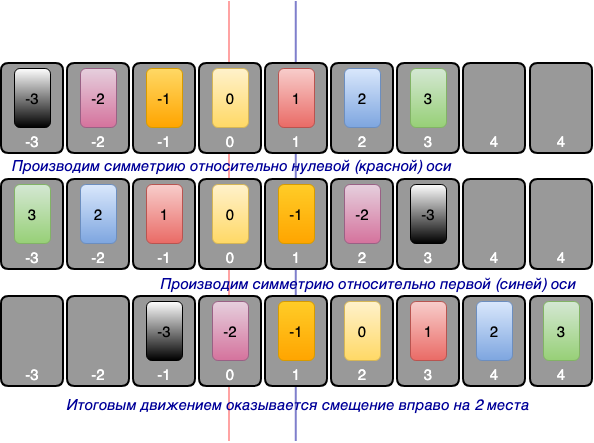
\includegraphics[scale=0.3]{SST.png}
\end{center}
\caption{}\label{SST}
\end{figure}
\item Заметим, что и в этом случае расстояние между а/м сохранится: как было ранее 2 а/м между 0-м и 3-м, так и останется. И так для всех пар автомобилей.
\item Такой вид движений называется \textbf{отражением}. Вся наша линейная парковка отразилась относительно нулевого места.
\item Особо отметим, что физически отражение всегда требует выхода за пределы исходной фигуры. Если сдвиг мы могли осуществить, находясь внутри парковочной сетки (ну, да, предположим, что мы имеем дело с танками, которые могут на месте повернуться на 90 градусов, произвести перемещение, а затем развернуться снова, либо что имеем дело с параллельной парковкой, где а/м стоят вдоль направления нумерации), то отражение никак невозможно выполнить, оставаясь в пределах исходной парковки --- потребуется выезд на проезжую часть.
\item Отражение на геометрической прямой --- то же самое. Сначала мы должны выбрать центр отражения, который останется на месте, затем перевернуть прямую в обратном направлении (снова имеем выход во внешнее пространство, если представить отражение как физический процесс!).
\item Отражение с центром в точке $O$ будем обозначать $S_O$. Отражение можно представить как огромное количество сдвигов, выполняемых одновременно. Для каждой точки --- свой сдвиг, причем на разные векторы для разных точек. Так, в результате действия отражения $S_O$ на точку $A$ мы получим точку $A'=T_a(A)$, где вектор $a=2\vec{AO}$. То есть, мы производим сдвиг на расстояние $2|OA|$, только в противоположную от $A$ сторону.
\item Как и в случае со сдвигом, отражение --- это функция, т.е. оно <<помнит>> исходную разметку прямой, а значит, мы всегда можем сказать, какая точка откуда пришла в свое новое состояние.
\item Отражение, в отличие от сдвига, намертво привязано к одной выделенной точке на прямой \textit{в исходной разметке}, и полностью ею определяется! Мы можем рассмотреть два и более отражений, но все они должны быть заданы в одной исходной разметке прямой, чтобы не возникла путаница.
\item Композиция отражений и композиция отражения и сдвига определяются аналогично композиции сдвигов (см. \eqref{Tcomposition}):
$$
(S_O\circ S_A)(x) = S_O(S_A(x)),\quad (S_O\circ T_a)(x) = S_O(T_a(x)),\quad (T_a\circ S_O)(x) = T_a(S_O(x)),
$$
т.е. применение операций выполняется справа налево.
\item Отражение обратно самому себе: $S_O\circ S_O=\id$, т.е. $S_O^{-1}=S_O$.
\item В терминах парада, показанного на рисунке, все отражения задаются относительно разметки мест на асфальте! В этом случае водителям для выполнения операции отражения не нужно знать, где какие номера а/м находятся, им достаточно видеть номер своего парковочного места, знать номер места---центра симметрии, и выполнить перемещение на удвоенное расстояние, чтобы занять противоположное место (см. рис. \ref{SST}).
\item Поэтому композиция отражений, т.е. их последовательное применение, легко вычисляется:
\begin{equation}\label{SOSC}
S_O\circ S_C=T_{2CO},\quad S_C\circ S_O=T_{2OC}.
\end{equation}
Если вспомнить общее групповое правило $(u\circ v)^{-1} = v^{-1}\circ u^{-1}$, то второе равенство легко получить из первого:
$$
T_{2OC} = T_{2CO}^{-1} = (S_O\circ S_C)^{-1} = S_C^{-1}\circ S_O^{-1}=S_C\circ S_O.
$$
\item Заметим, что композиция отражений является сдвигом и при этом не коммутативна! То есть, отражения, производимые в разной последовательности, приводят, вообще говоря, к разным результирующим сдвигам, а именно --- к противоположным.



\section{Таблица композиций движений прямой}


\lesson{Составляем композиции отражений и сдвигов. Таблица композиций классов, аналог таблицы умножения знаков}


\item Композиция отражения и сдвига:
\begin{equation}\label{SOTa}
S_O\circ T_a = S_{O-a/2},\quad T_a\circ S_O = S_{O+a/2}.
\end{equation}

Это легко проверить, если вместо $a$ подставить $2CO$, и в предыдущих равенствах произвести необходимые домножения. Предлагаем это проделать самостоятельно.
\item Итак, композиция сдвига и отражения является отражением и при этом не коммутативна!
\item Таблица композиций отражений и сдвигов:\index{Группа!движений прямой}
\begin{center}
\begin{tabular}{c|c|c|}
  & $T_a$ & $S_O$ \\
 \hline
$T_b$ & $T_{a+b}$ & $S_{O+b/2}$ \\
 \hline
$S_C$ & $S_{C-a/2}$ & $T_{2OC}$ \\
\hline
\end{tabular}
\end{center}
Таблицу композиций следует читать слева наверх, т.е. если в левом столбце стоит движение $F$, а в верхней строке --- движение $G$, то в соответствующей ячейке стоит композиция $F\circ G$.
\item Кратность отражения $S_O^n$ определяется четностью числа $n$. В случае четного $n$ это $\id$, в случае нечетного --- исходное $S_O$.
\item Пара $\{\id, S_O\}$ образует самую маленькую нетривиальную группу движений, которая, к тому же, является абелевой и циклической (т.е. все ее элементы есть степени какого-то одного, а именно $S_O=S_O^1$, $\id=S_O^2=S_O^0$).
\begin{table}[htb!]\begin{center}
\begin{tabular}{c|c|c|}
  & $\id$ & $S_O$ \\
 \hline
$\id$ & $\id$ & $S_O$ \\
 \hline
$S_O$ & $S_O$ & $\id$ \\
\hline
\end{tabular}
\end{center}\end{table}
\item Видим, что таблица полностью повторяет таблицу умножения знаков, причем $\id$ является нейтральным элементом.
\item Суммируя, находим, что вообще все сдвиги и отражения вместе образуют группу (относительно операции композиции), т.е. для них выполняются аксиомы группы G1--G4. При этом данная группа не является абелевой (не выполняется G5), поскольку, как мы видели, далеко не все композиции движений перестановочны.
\item Еще пример группы: рассмотрим класс всех сдвигов $\T$ и класс всех отражений $\S$
\item Мы можем определить композицию классов $\T\circ \T$, $\T\circ \S$, $\S\circ \T$ и $\S\circ \S$ как все возможные композиции движений из этих классов в указанном порядке. Иначе говоря, композиции классов --- это их умножение по Минковскому:
$$
\T\circ \T = \{t\circ t'\mid (t\in\T)\land(t'\in\T)\},\quad \T\circ \S = \{t\circ s\mid (t\in\T)\land(s\in\S)\}
$$
$$
\S\circ \T = \{s\circ t\mid (s\in\S)\land(t\in\T)\},\quad \S\circ \S = \{s\circ s'\mid (s\in\S)\land(s'\in\S)\}
$$
\item Из произведенных выше вычислений легко видеть таблицу композиций этих классов:\index{Таблица композиций}
\begin{center}
\begin{tabular}{c|c|c|}
  & $\T$ & $\S$ \\
 \hline
$\T$ & $\T$ & $\S$ \\
 \hline
$\S$ & $\S$ & $\T$ \\
\hline
\end{tabular}
\end{center}
\item Видим полную аналогию с таблицей знаков и таблицей для $\id, S_O$. Здесь класс $\T$ является нейтральным элементом
\item Если теперь собрать в одну кучу все сдвиги и отражения, то получим группу движений прямой
\item Наша цель --- доказать, что других движений нет, т.е. что мнжество $\{T_a,S_O\}_{a,O}$ полностью исчерпывает все возможные движения прямой
\end{enumerate}

\subsection*{Задачи}

Пусть на прямой даны 4 точки $A,B,C,D$, поставленные друг за другом с одинаковым шагом (см. рис. \ref{ABCD}).
\begin{figure}[hbt!]
\begin{center}
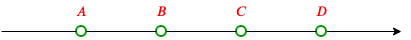
\includegraphics[scale=0.7]{ABCD.png}
\end{center}
\caption{}\label{ABCD}
\end{figure}

\begin{enumerate}
\item Куда перейдет точка $A$ при преобразовании $S_B$?
\item Куда перейдут точки $B,C,D$ при преобразовании $T_{AB}\circ T_{CA}$?
\item Куда перейдут точки $A,B,C$ при преобразовании $S_C\circ T_{AB}$?
\item Вывести равенства \eqref{SOTa} из равенств \eqref{SOSC}.
\end{enumerate}



\section{Теорема о гвоздях, аналог теоремы Шаля}


\lesson{Стационарные точки. Теорема Шаля}


\begin{enumerate}
\item Анализ движений проводится на основе наблюдений за количеством стационарных точек
\item Пусть движение $M$ таково, что оно оставляет на месте две точки $A\ne B$.
\item $M(A)=A$ и $M(B)=B$. Пусть $C'=M(C)$. $M$ сохраняет расстояния $AC$ и $BC$, откуда $AC=AC'$ и $BC=BC'$, откуда $C=C'$. Т.е. $M(C)=C$ для любых точек $C$, т.е. $M=\id$

\begin{figure}[hbt!]
\begin{center}
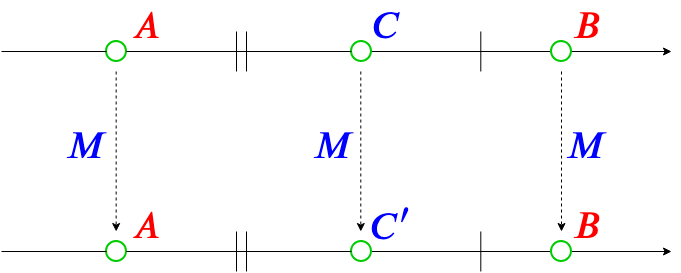
\includegraphics[scale=0.35]{LineMoving.png}
\end{center}
\caption{}\label{LineMoving}
\end{figure}
\item Пусть движение $M$ оставляет на месте ровно одну точку $O$. В этом случае $A'=M(A)$ и $A\ne A'$ и $OA=OA'$, тогда $A'$ --- отражение $A$ относительно $O$. Следовательно, $M=S_O$
\begin{figure}[hbt!]
\begin{center}
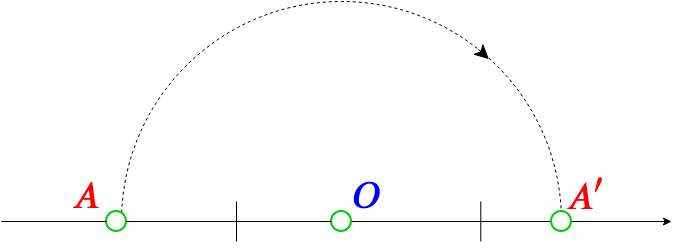
\includegraphics[scale=0.35]{LineMovingO.png}
\end{center}
\caption{}\label{LineMovingO}
\end{figure}

\item Пусть движение $M$ не оставляет на месте ни одной точки и пусть $B=M(A)$ ($B\ne A$). Обозначим $x=AB$. Тогда $T_{x}^{-1}\circ M(A)=A$, т.е. $T_{x}^{-1}\circ M$ оставляет на месте хотя бы одну точку $A$.
\begin{figure}[hbt!]
\begin{center}
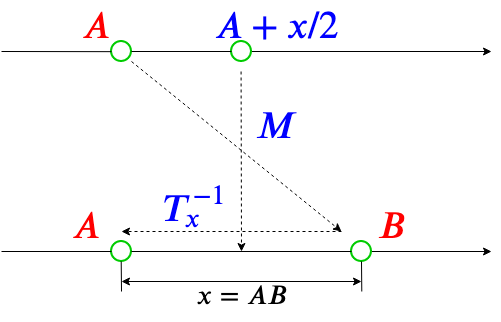
\includegraphics[scale=0.35]{LineMovingx.png}
\end{center}
\caption{}\label{LineMovingx}
\end{figure}

Если оно оставляет на месте ровно одну точку $A$, то это некоторое отражение $S_A$, но тогда $M=T_x\circ S_A=S_{A+x/2}$. Получается, что $M$ сохраняет точку $A+x/2$ на месте. Противоречие. Остается вариант, что $T_{x}^{-1}\circ M$ оставляет на месте как минимум две точки, но тогда $T_{x}^{-1}\circ M=\id$, откуда $M=T_x\circ \id=T_x$ --- сдвиг.
\item Таким образом, все движения прямой --- это либо сдвиги (в частности, $\id$), либо отражения (теорема Шаля).\index{Теорема!Шаля}
\item При этом любое движение --- это либо одно отражение, либо композиция двух отражений.
\end{enumerate}
\subsection*{Задачи}
\begin{enumerate}
\item Построить сдвиг на 7 единиц вправо с помощью композиции двух симметрий.
\item Каким движением является следующая композиция?
$$
S_{O+n}\circ S_{O+n-1}\circ \dots\circ S_{O+1}\circ S_O.
$$
Ответ получить в зависимости от четности $n$.
\end{enumerate}


\section{Все конечные подгруппы движений прямой}



\lesson{Описание всех вариантов, как может сложиться конечная подгруппа движений}

\begin{enumerate}
\item Имея дело с группой движений, мы можем выделить несколько ее собственных подгрупп (определение и разбор понятия подгруппы см. на стр. \pageref{Subgroup}):
\begin{itemize}
\item подгруппа всех сдвигов --- бесконечная коммутативная группа;
\item подгруппа, порожденная одним сдвигом $\langle T_a\rangle$ --- тоже бесконечная коммутативная группа;
\item подгруппа одного отражения $\{\id, S_O\}$ --- конечная группа, состоящая из двух элементов, также коммутативная;
\item тривиальная подгруппа $\{\id\}$.
\end{itemize}
\item Возникает вопрос: а существуют ли промежуточные по размеру конечные подгруппы группы движений? Попробуем описать все конечные подгруппы движений прямой.
\item Пусть $H$ --- конечная подгруппа группы движений прямой.

Ранее (см. стр.  \pageref{Subgroup}) мы рассматривали два определения подгруппы: 1) как подмножества, являющегося группой относительно той же операции, 2) как непустого подмножества $H$, в котором $ab^{-1}\in H$ при $a,b\in H$. В случае конечной подгруппы определение можно упростить еще больше, а именно, заменить $ab^{-1}$ на банальное $ab$.

Итак, непустое конечное(!) подмножество $H$ группы $G$ образует подгруппу группы $G$, если для любых $a,b\in H$ имеет место $ab\in H$, т.е. если $H$ замкнуто относительно групповой операции.

Почему это так? Здесь нам на помощь приходит принцип Дирихле. Пусть в множестве $H$ ровно $n$ элементов ($n>0$). Возьмем какой-то элемент $h\in H$ и рассмотрим все его натуральные степени относительно групповой операции: $h, h\circ h, h\circ h\circ h$ и т.д. Ясно, что мы можем построить сколь угодно длинные композиции, в том числе, содержащие $n$ и более вхождений элемента $h$. Возьмем тогда первые $n+1$ таких композиций. Все они, по условию, являются элементами множества $H$, т.е. совпадают с одним из его $n$ элементов. Но тогда в силу принципа Дирихле найдется как минимум две равных композиции. Пусть в одной из них $k$ вхождений $h$, а в другой $j$, причем $k<j$:
$$
\underbrace{h\circ h\circ\dots\circ h\circ h}_{k} = \underbrace{h\circ h\circ\dots\circ h\circ h}_{j}.
$$
Пользуясь тем, что в группе $G$ есть обратный элемент $h^{-1}$, домножим это равенство справа $k$ раз на $h^{-1}$, в итоге получим
$$
\id = \underbrace{h\circ h\circ\dots\circ h\circ h}_{j-k}.
$$
Справа --- композиция элементов из $H$, а значит, принадлежит $H$, откуда следует, что $\id$ исходной группы $G$ находится в $H$. Далее, мы можем еще раз умножить полученное равенство на $h^{-1}$, и получим
$$
h^{-1} = \underbrace{h\circ h\circ\dots\circ h\circ h}_{j-k-1},
$$
где $j-k-1\ge 0$. Справа --- либо композиция элементов из $H$, либо $\id$, который также принадлежит $H$ по доказанному. Но тогда и $h^{-1}\in H$. Так что, всякий элемент входит в $H$ вместе со своим обратным. А отсюда уже следует, что $H$ удовлетворяет второму определению подгруппы, и по доказанному на стр. \pageref{Subgroup} является группой с той же операцией и единицей, что и в группе $G$.

\item Итак, пусть $H$ --- непустое конечное подмножество группы движений прямой, замкнутое относительно операции композиции. Как мы только что выяснили, $H$ является подгруппой группы движений.

Таким образом, во-первых, $\id$ есть элемент $H$.

\item Во-вторых, никакой сдвиг $T_a$ при ненулевом $a$ не может быть элементом $H$, иначе в $H$ окажутся все степени $T_a$, т.е. $\langle T_a\rangle \subseteq H$, и $H$ будет бесконечной.
\item В-третьих, если в $H$ есть хотя бы два различных отражения $S_A$ и $S_B$ ($A\ne B$), то и их композиция также находится в $H$, но это ненулевой сдвиг $T_{2AB}$, а все такие сдвиги мы исключили чуть выше. Следовательно, если в группе $H$ и есть отражение, то только одно.
\item Таким образом, либо $H=\{\id\}$ (тривиальная группа), либо $H=\{\id, S_O\}$ при некотором отражении $S_O$.
\end{enumerate}


\newchapter{Вокруг окружности}

\vrezka{В этой главе мы расширяем сферу деятельности и переходим к движениям окружности. Снова изучаем виды движений, строим таблицу композиций, доказываем теорему Шаля.

Попутно сопоставляем движения окружности с движениями прямой, выходим на отрицательные степени композиций и их арифметические свойства, как следствие, получаем целые числа другим путем.

По аналогии с натуральными числами говорим о том, что целые числа --- это и степени композиций движений, и мера длины, только оснащенная знаком, т.е. направлением измерения длины.
}

\section{Движения окружности}


\lesson{Иллюстрация движений окружности: повороты и отражения. Некоторые повороты, примененные несколько раз, дают нулевой поворот. Композиция поворотов}

\begin{enumerate}
\item \textbf{Иллюстративная сказка}. Вспомним песенку <<встаньте, дети, встаньте в круг!>> Представим, что много-много детей в спортивном зале выстроились в круг и начали водить хоровод. При этом в центре круга стоит воспитательница, так что все дети держатся на равном от нее расстоянии и смотрят на нее. Какое они осуществляют движение в зале? Они ходит под одной и той же окружности то в одну сторону, то в другую. И если мы поместим себя на место воспитательницы, то поймем, что хоровод просто вращается вокруг одного центра то влево, то вправо.\index{Движения!окружности}

Добавим к этому мероприятию драйва. В зале на полу прочерчена линия, которая делит его пополам на два прямоугольника. По хлопку в ладоши дети перебегают на противоположную сторону зала, т.е. они все бегут по прямым параллельным линиям, перпендикулярно линии, нарисованной на полу (примерно так же люди переходят зебру при переходе улицы по зеленому сигналу светофора). При этом каждый из них считает число шагов до линии, а затем продолжает движение в том же направлении еще на столько же шагов. Дойдя до конца, все разворачиваются так, чтобы снова видеть воспитательницу.

В итоге они снова образуют круг, только вывернутый наизнанку, т.к. у каждого участника круга сосед, стоявший слева, теперь стоит справа, и наоборот! Такое действие с кругом называется отражением. При этом, тот факт, что соседи поменялись местами, говорит нам о некотором необычном движении, а именно, о движении, меняющем ориентацию (перепутали право и лево).

\item Формализуем это с геометрической точки зрения. Берем окружность. Какие у нее есть движения, переводящие ее в саму себя?
\item Прежде всего, повторим, что движение --- это преобразование, сохраняющее расстояния (изометрия). Поэтому, если мы говорим о движении, переводящем фигуру (прямую, круг, квадрат, многоугольник, плоскость и т.д.) в саму себя, то это значит, что мы берем копию этой фигуры и накладываем ее на оригинал до полного совмещения контуров. При этом допускается вертеть ее как угодно, лишь бы наложение фигур оказалось идеальным --- без выступов и впадин, без какой-либо деформации.
\item Для того, чтобы уточнить смысл определения движения, нужно зафиксировать способ измерения расстояний на окружности.  Расстоянием между точками окружности $A$ и $B$ мы будем называть длину меньшей из дуг, соединяющих эти точки (вместо длины дуги можно использовать величину соответствующего ей угла, измеренного в радианах или градусах).
\item Очевидно, что движениями окружности являются как минимум: вращение вокруг ее центра, а также отражение относительно прямых, проходящих через ее центр.
\item В некотором смысле окружность --- аналог прямой. Только эту прямую взяли за 2 конца и замкнули где-то на бесконечности.
\item Поэтому вращение окружности соответствует сдвигу прямой, а отражение окружности относительно прямой --- отражению на прямой относительно точки (можно считать ее отражением относительно перпендикулярной прямой).
\item Если представить, что на окружности большого радиуса живут маленькие одномерные математики, то для них окружность будет практически не отличима от прямой, и движения окружности они будут воспринимать именно как движения прямой.
\item Поворот на угол $\al$ мы обозначим за $R_\al$ (положительный --- против часовой стрелки), отражение относительно прямой, имеющей угол наклона $\ph$, обозначим за $S_\ph$ ($0\le\ph<180^o$). Угол наклона прямой измеряется от заданного раз и навсегда радиуса окружности, который можно считать точкой отсчета (аналог нуля на прямой). В качестве радиуса нулевого угла мы выберем горизонтальный радиус справа от центра окружности.
\item Ось отражения $S_\ph$ мы будем обозначать $l_\ph$ (см. рис. \ref{Rund3}).

\begin{figure}[hbt!]
\begin{center}
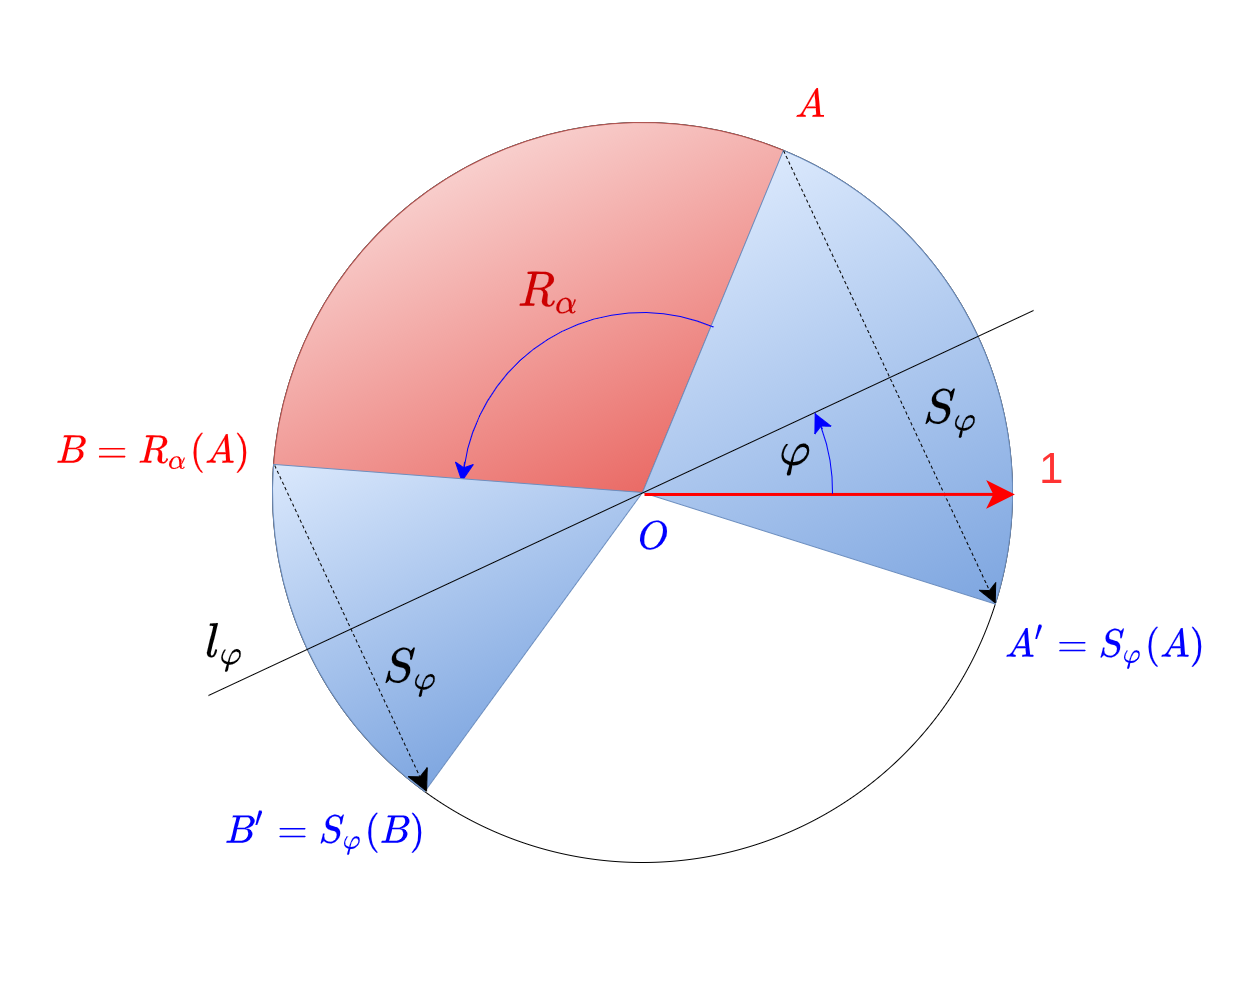
\includegraphics[scale=0.2]{Rund3.png}
\end{center}
\caption{}\label{Rund3}
\end{figure}

\item Вновь замечаем, что композиция поворотов есть поворот на суммарный угол: $R_\al\circ R_\be=R_{\al+\be}$
\item У каждого поворота есть обратный: $R_\al^{-1}=R_{-\al}$, т.н. поворот в противоположном направлении.
\item Повороты коммутируют: $R_\al\circ R_\be=R_\be\circ R_\al$.
\item Есть нейтральный поворот $\id=R_0$.
\item Так что все повороты образуют группу относительно операции композиции.
\item Тем не менее, есть одна особенность: поворот на угол $360^o$ (и все углы, кратные ему) --- это тоже $\id$.
\item Вообще, повороты, заданные углами с шагом $360^o$, равны друг другу:
$$
R_\al=R_{\al\pm 360^ok},
$$
где $k$ --- натуральное число.
\item Некоторые повороты дают $\id$ в некоторой степени, например, $R_{90^o}^4=\id$, $R_{60^o}^6=\id$ и т.д.
\item Если угол, выраженный в градусах, соизмерим с величиной $360^o$, то поворот на данный угол имеет положительную степень, в которой он обращается в $\id$.

Действительно, соизмеримость угла $\ph$ с углом $360^o$, как мы определяли ранее, означает, что существует некоторый угол $\psi$, кратный как $\ph$, так и $360$, т.е.
$$
\psi = \ph m = 360n.
$$
Но это и означает, что поворот $R_\ph$, возведенный в степень $m$, даст угол, кратный $360^o$, т.е. $\id$.

\item Но есть и такой угол $\ph$, который не соизмерим с углом $360^o$, и потому ни в какой степени не может дать $\id$. Это угол в 1 радиан.

Определение: угол $\ph$ равен 1 радиану, если длина дуги окружности, соответствующая данном углу, в точности равна радиусу этой окружности.

Когда угол измеряется в радианах, имеется ввиду, что мера угла есть длина соответствующей этому углу дуги единичной окружности. В частности, развернутому углу соответствует половина длины единичной окружности, обозначаемая числом $\pi$, так что угол $180^o$ --- это $\pi$ радиан.

Если бы угол в 1 радиан был соизмерим с полным оборотом, то число $\pi$ также оказалось бы соизмеримым с 1. Известно, однако, что это не так! Доказательство этого факта является сложной математической теоремой!

В свете сказанного, получем, что сколько бы раз мы ни откладывали угол в 1 радиан на окружности, мы никогда не окажемся в точке, соответствующей нулевому углу. Соответственно, группа вращений, порожденная степенями $R_{1\rad}$, является бесконечной. Позже мы докажем теорему о том, что углы поворота из этой группы образуют плотное множество, т.е. этими углами можно с любой точностью приблизить поворот на любой угол.

\item В зависимости от соизмеримости угла поворота с полным оборотом некоторые повороты порождают конечные циклические подгруппы в группе движений, а некоторые --- нет.
\end{enumerate}


\section{Группа движений окружности, теорема Шаля}

\lesson{Композиция отражений окружности. Таблица композиций движений окружности}

\begin{enumerate}\setlength{\itemsep}{1pt}
\item Композиция отражений: 
\begin{equation}\label{SSR}
S_\psi\circ S_\ph=R_{2(\psi-\ph)},\quad S_\ph\circ S_\psi=R_{2(\ph-\psi)}
\end{equation}
Например, второе равенство легко увидеть из картинки \ref{Rund}, где точка $A$ переходит в $A'$ под действием отражения $S_\psi$ относительно оси $l_\psi$, а затем $A'$ переходит в $A''$ под действием отражения $S_\ph$ относительно оси $l_\ph$:

\begin{figure}[hbt!]
\begin{center}
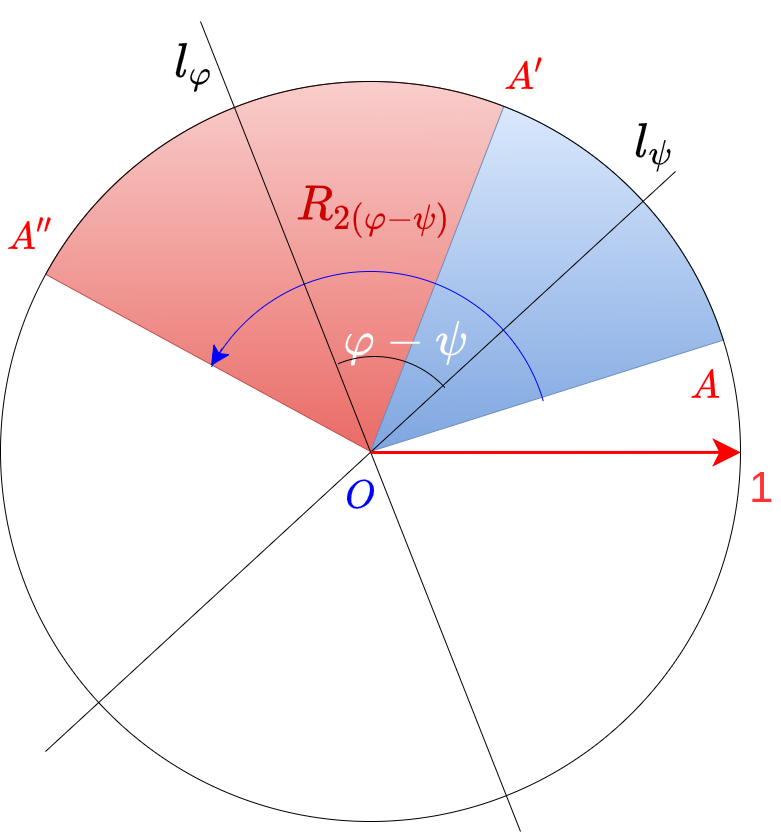
\includegraphics[scale=0.25]{Rund.png}
\end{center}
\caption{}\label{Rund}
\end{figure}

Суммарный угол поворота точки $A$ при переходе в точку $A''$ можно разбить на 2 пары углов так, что в каждой паре углы равны в силу свойств отражения (разные пары отмечены разным цветом), и в то же время угол между осями состоит как раз из суммы углов, принадлежащих разным парам. Нетрудно убедиться в аналогичном результате и в том случае, если точка лежит между осями отражений.

\item Итак, композиция отражений является поворотом на двойной угол между их осями. Отсюда видно также, что композиция отражений не коммутативна! Перестановка отражений приводит к смене направления вращения.
\item Композиция отражения и поворота:
\begin{equation}\label{SRS}
S_\ph\circ R_\al = S_{\ph-\al/2},\quad R_\al\circ S_\ph = S_{\ph+\al/2}
\end{equation}

Рассмотрим композицию $S_\ph\circ R_\al$. Пусть также $\psi = \ph-\al/2$.
Из \eqref{SSR} получаем, что
$$
S_\ph\circ S_\psi = R_{2(\ph-\psi)}=R_\al,
$$
после чего умножаем это равенство слева на $S_\ph$ и, пользуясь тем, что $S_\ph\circ S_\ph=\id$, находим, что:
$$
S_\psi = S_\ph\circ R_\al,
$$
откуда, производя замену $\psi=\ph-\al/2$, окончательно получаем, что
$$
S_\ph\circ R_\al = S_{\ph-\al/2}
$$

Аналогично доказывается второе равенство.
\item Итак, композиция отражения и поворота является отражением и при этом тоже не коммутативна!
\item Запишем полную таблицу композиций отражений и вращений окружности:\index{Группа!движений окружности}
\begin{center}
\begin{tabular}{c|c|c|}
  & $R_\al$ & $S_\psi$ \\
 \hline
$R_\be$ & $R_{\al+\be}$ & $S_{\psi+\be/2}$ \\
 \hline
$S_\ph$ & $S_{\ph-\al/2}$ & $R_{2(\ph-\psi)}$ \\
\hline
\end{tabular}
\end{center}
\item По аналогии с прямой обозначим за $\T$ класс всех вращений окружности, за $\S$ --- класс всех отражений окружности.
\item Получаем аналогичную таблицу композиций классов:
\begin{center}
\begin{tabular}{c|c|c|}
  & $\T$ & $\S$ \\
 \hline
$\T$ & $\T$ & $\S$ \\
 \hline
$\S$ & $\S$ & $\T$ \\
\hline
\end{tabular}
\end{center}

\item Снова наблюдаем все ту же группу умножения знаков!


\lesson{Доказываем, что других движений окружносмти нет. Теорема Шаля}


\item Существуют ли другие движения окружности? Ответ --- нет!
\item Анализ движений проводится, как и в случае прямой, на основе наблюдений за количеством стационарных точек.
\item Для начала заметим, что если при движении окружности одна точка остается на месте, то неподвижной будет и диаметрально противоположная ей точка. Если бы это было не так, то, очевидно, расстояние между этими точками (равное половине дуги окружности) не сохранялось бы --- оно стало бы меньше. А это невозможно при движении.
\item Поэтому при анализе движений окружности всегда нужно иметь в виду, что пары противоположных точек ведут себя одинаково --- либо они обе стационарны, либо обе двигаются.
\item Пусть движение $M$ таково, что оно оставляет на месте две точки $A\ne B$, не являющиеся диаметрально противоположными.
\item Тогда, во-первых, $M(A)=A$ и $M(B)=B$. Пусть $C$ --- еще какая-то точка и $C'=M(C)$. Здесь могут быть два варианта: либо $C$ лежит на малой дуге $AB$, либо на большой. Эти дуги не могут быть равны по длине, т.к. $A$ и $B$ не являются противоположными (см. рис. \ref{Rund1}). Точка $C'$ тоже может лежать строго на одной из этих дуг.

Поскольку $M$ сохраняет расстояния, дуги $AC$ и $AC'$ равны, дуги $BC$ и $BC'$ равны. А значит, равны и суммы длин дуг $AC+CB$ и $AC'+C'B$. Отсюда следует, что $C$ и $C'$ могут лежать только на одной и той же дуге. Но тогда, в силу равенства дуг $AC$ и $AC'$ точки $C$ и $C'$ также должны совпадать (они лежат на одной дуге и на равных расстояниях от концов). Таким образом, $M(C)=C$ для любых точек $C$, т.е. $M=\id$.

\begin{figure}[hbt!]
\begin{center}
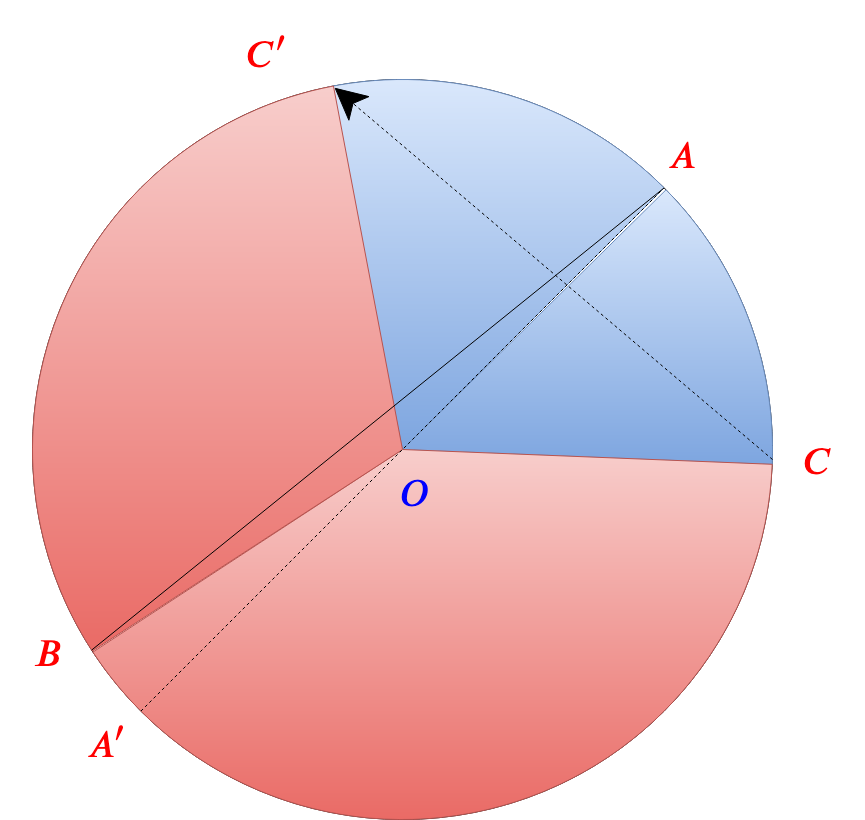
\includegraphics[scale=0.25]{Rund1.png}
\end{center}
\caption{}\label{Rund1}
\end{figure}
\item Пусть движение $M$ оставляет на месте ровно одну пару противоположных точек $A$ и $A'$ (см. рис. \ref{Rund1}).
Рассмотрим снова произвольную точку $C$ на окружности, отличную от $A$ и $A'$. И пусть $C'=M(C)$. Тогда $C\ne C'$ и $AC=AC'$. Отсюда следует, что $C'$ --- отражение точки $C$ относительно оси $AA'$. Следовательно, $M=S_\ph$, где $\ph$ --- угол наклона прямой $AA'$.
\item Пусть движение $M$ не оставляет на месте ни одной точки. Возьмем произвольную точку $A$ на окружности, и пусть $B=M(A)$ (по условию $B\ne A$). Обозначим за $\al$ угол дуги $AB$ (см. рис. \ref{Rund2}).

\begin{figure}[hbt!]
\begin{center}
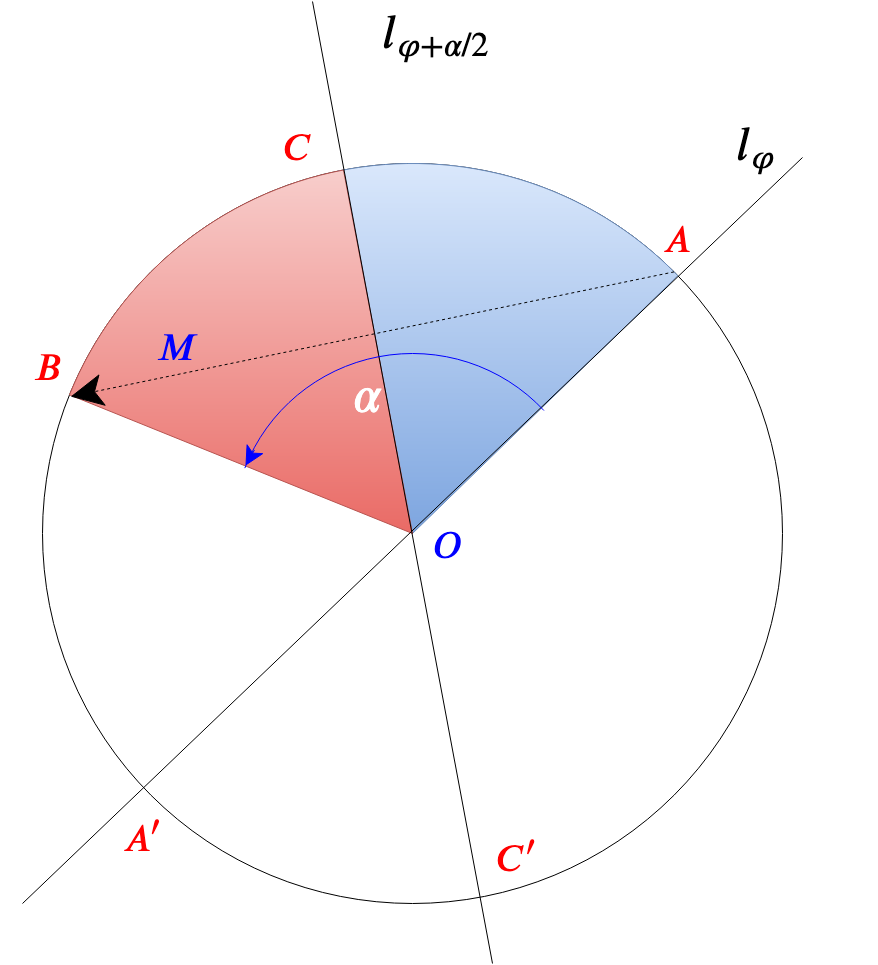
\includegraphics[scale=0.25]{Rund2.png}
\end{center}
\caption{}\label{Rund2}
\end{figure}
Тогда $R_{\al}^{-1}\circ M(A)=A$, т.е. $R_{\al}^{-1}\circ M$ оставляет на месте хотя бы одну точку $A$ (а точнее, пару противоположных точек $A$ и $A'$). Если оно оставляет на месте ровно одну пару точек $A$ и $A'$, то это некоторое отражение $S_\ph$ (на рис. \ref{Rund2} ось отражения обозначена за $l_\ph$), но тогда $M=R_\al\circ S_\ph=S_{\ph+\al/2}$ в силу второго равенства в \eqref{SRS}. Получается, что $M$ сохраняет точку $C$ на месте ($C$ есть середина дуги $AB$). Получаем противоречие с тем, что $M$ не оставляет на месте ни одной точки.

Остается вариант, что $R_{\al}^{-1}\circ M$ оставляет на месте как минимум две точки, не являющиеся противоположными, но тогда $R_{\al}^{-1}\circ M=\id$ (по доказанному ранее), откуда $M=R_\al\circ \id=R_\al$ --- поворот.

\item Таким образом, всякое движение окружности --- это либо поворот (в частности, $\id$), либо отражение относительно оси, проходящей через центр окружности (теорема Шаля).\index{Теорема!Шаля}
\item При этом любое движение окружности --- это либо одно отражение, либо композиция двух отражений.
\end{enumerate}
\subsection*{Задачи}
\begin{enumerate}
\item Центральная симметрия --- это какое движение?
\item Композицией каких отражений можно выразить центральную симметрию?
\item С помощью отражения относительно оси $Ox$ и вращений выразить отражение относительно оси $Oy$.
\end{enumerate}


\section{Наматывание прямой на окружность}

\lesson{Совмещаем вращение окружности и движение прямой: колесо на дороге. Шкала натуральных чисел соответствует полным оборотам колеса. Вращение в разные стороны соответствует положительным и отрицательным, т.е. целым числам. Определение разности чисел и отрицательной степени поворота окружности и сдвига. Концепция целых чисел как степеней сдвигов и поворотов без ограничений в ту или другую сторону.}

\begin{enumerate}
\item Совместим теперь окружность с прямой иным способом. Выделим на окружности точку $O$ и начнем ее обход (вращение) в положительном направлении.
\item Выше мы видели, что углы поворота, кратные $360^o$, т.е. полному обороту, соответствуют тождественному движению, т.е. приведут нас в точку отправления $O$.
\item Однако, если с точки зрения математического движения ничего не изменилось, физически мы проделали путь, равный длине окружности. Для удобства будем считать, что радиус окружности есть единичный вектор, так что ее длина равна $2\pi$, и с каждым полным оборотом мы будем <<наматывать>> расстояние $2\pi$.
\item Более общо, расстояние, пройденное по окружности единичного радиуса, когда этот радиус заметает угол $\al$, равно $\al(2\pi/360^o)$. Чтобы каждый раз не переводить единицы измерения радиуса в градусы и наоборот, углы также принято измерять в единицах длины --- радианах. А именно, \textit{угол в} 1 \textit{радиан соответствует повороту, при котором точка проделает по окружности путь, равный по длине радиусу данной окружности}. Нетрудно видеть, что в градусах 1 радиан будет иметь выражение $360^o/(2\pi)$ или $180^o/\pi \approx 57^o$.
\item В дальнейшем условимся все углы измерять в радианах, если не оговорено иное.
\item Известно, что число $\pi$ не соизмеримо с целыми числами (как уже отмечалось, этот факт является довольно сложной теоремой), так что поворот $R_1$ на 1 радиан ни в какой положительной степени не приведет нас снова в точку исхода $O$.
\item Зато поворот $R_{2\pi}$ в точности возвращает нас в точку отправления $O$.
\item При каждом таком повороте мы проделываем путь, равный углу поворота, т.е. $2\pi$ (радиус равен 1).
\item Следовательно, степени такого поворота $R_{2\pi}^n$ дадут прохождение пути длиной $2\pi n$.
\item Представим эту картину не с точки зрения жителей окружности, бегающих по замкнутой траектории, а с точки зрения жителей прямой, которая наматывается на окружность. С их точки зрения все выглядит несколько иначе и больше напоминает движение колеса по дорожному полотну: окружность катится по прямой и через равные промежутки касается точкой $O$ данной прямой.
\item Если при этом два друга --- один из мира окружности, второй из мира прямой, --- двигаются с одинаковой скоростью в одном направлении, то они могут синхронизироваться в точке касания окружности и прямой и разговаривать друг с другом, постоянно двигаясь каждый по своему объекту, но вместе.
\item Нужно заметить при этом, что если колесо вращается по часовой стрелке, т.е. в отрицательном направлении, то вдоль прямой оно движется направо, т.е. в положительном направлении. Но фокус в том, что житель окружности для синхронизации с жителем прямой должен идти навстречу вращению колеса, т.е. тоже в положительном направлении! Таким обраом, движения обоих друзей имеют одинаковый знак! На рис. \ref{RundLine} мы отметили синей стрелкой направление движения жителя окружности, а черной --- встречное вращение самой окружности.
\item Итак, колесо катится, два друга беседуют, точка $O$ то и дело, а именно, через каждые $2\pi$ метров соприкасается с прямой. Каждый раз, когда точка $O$ касается прямой, наш ученый друг из мира прямой ставит на ней отметины и считает их по порядку, т.е. приравнивает к степени совершенного поворота колеса: в начальный момент времени это был 0, затем 1 оборот, затем 2 оборота, и т.д.

\begin{figure}[hbt!]
\begin{center}
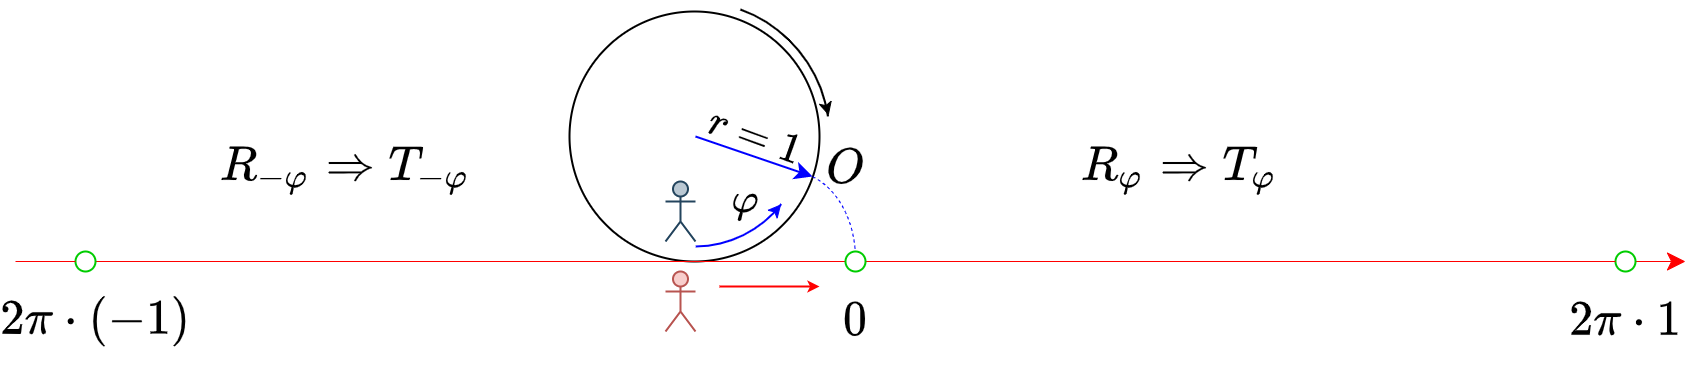
\includegraphics[scale=0.2]{RundLine.png}
\end{center}
\caption{}\label{RundLine}
\end{figure}

\item Что же мы видим на прямой? Мы видим не что иное как шкалу натуральных чисел, в точности соответствующую степеням вращений окружности. Число $2\pi$, фигурирующее как коэффициент, является не более чем единицей измерения. Кто-то измеряет в метрах, кто-то -- в ярдах, а мы измеряем в длинах единичной окружности.
\item Представим теперь, что в какой-то момент касания точки $O$ с прямой физика мира изменилась, и вращение начало осуществляться в обратную сторону!
\item Наши друзья-ученые при этом продолжат совместное путешествие, но только назад. Они пойдут отсчитывать уже проставленные отметки на прямой в убывающем порядке, пока не вренутся в точку 0. Но здесь процесс не остановится, и движение продолжится дальше.
\item Как все это записать на языке вращений и сдвигов?
\item Предположим, что сначала окружность повернулась на $n$ полных оборотов вперед, а затем на $m$ полных оборотов назад (см. рис. \ref{RundLine1}).
\item Мы получаем итоговое вращение, записываемое как $R_{2\pi n}\circ R_{2\pi m}^{-1}$.
\item А что мы имеем с точки зрения движения на прямой?
\item Сначала был произведен сдвиг $T_{2\pi n}$, затем сдвиг $T_{-2\pi m}$.
\item И мы видим, что индекс, определяющий итоговое вращение и итоговый сдвиг, --- один и тот же!
\item Причем, если $n>m$, то сдвиг жителя прямой будет вправо на расстояние $2\pi(n-m)$, а поворот жителя окружности будет положительным на угол $2\pi(n-m)$.
\item Если же $n<m$, то сдвиг жителя прямой будет влево на расстояние $2\pi(m-n)$, а поворот жителя окружности будет отрицательным (по часовой стрелке) на угол $2\pi(m-n)$.
\item Ранее мы уже договаривались, что перед векторами, направленными влево, будем ставить знак '-'. Так же мы будем поступать и с углами вращений в отрицательную сторону.
\item Соответственно, при $n<m$ мы будем иметь итоговый сдвиг на прямой $T_{-2\pi(m-n)}$ и итоговый поворот на окружности $R_{-2\pi(m-n)}$, которые также можно записать в виде степеней:
$$
T_{-2\pi(m-n)}=T_{2\pi}^{-(m-n)}\mbox{ и }R_{-2\pi(m-n)}=R_{2\pi}^{-(m-n)}.
$$

\begin{figure}[hbt!]
\begin{center}
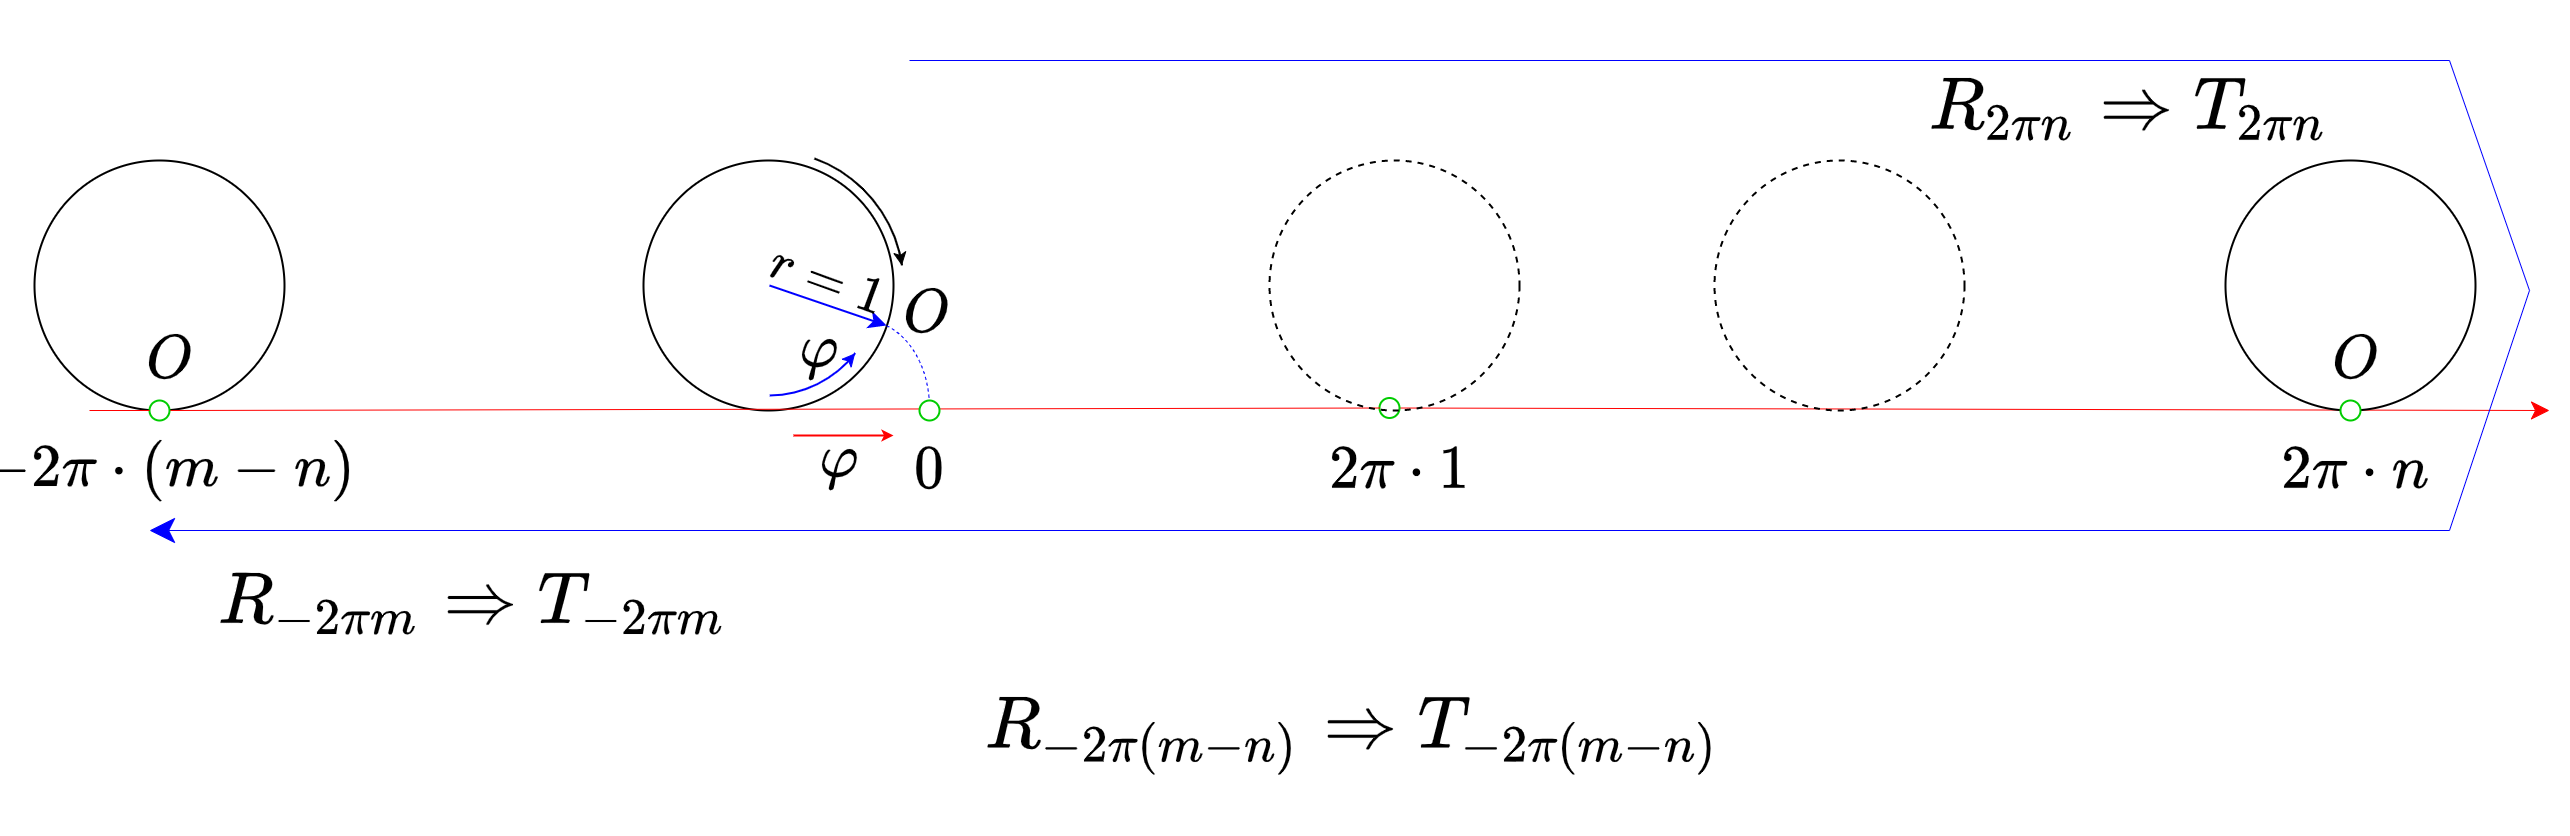
\includegraphics[scale=0.15]{RundLine1.png}
\end{center}
\caption{}\label{RundLine1}
\end{figure}

\item Осталось добавить маленький штрих к портрету, а именно: в случае $n<m$ под разностью $n-m$ будем понимать запись $-(m-n)$.
\item Тогда уже независимо от того, $n<m$, или $m<n$, или $n=m$, композиция поворотов и сдвигов сначала на $n$ вправо и затем на $m$ влево будет записываться одинаково:
$$
T_{2\pi(n-m)}=T_{2\pi}^{n-m}\mbox{ и }R_{2\pi(n-m)}=R_{2\pi}^{n-m}.
$$
\item В итоге мы приходим к тому, что называется \textbf{целыми числами}, включающими натуральные числа и отрицательные натуральные числа (при этом $-0=0$).
\item Сколько бы мы ни вращали окружность на $2\pi$ в ту или иную сторону с помощью поворота $R_{2\pi}$, мы совершаем поворот на целую степень полного оборота. При этом как бы мы ни катали окружность по прямой, точка $O$ будет ставить отметки в точках $2\pi k$, где $k$ --- целое число.
\end{enumerate}






\newchapter{Целые числа и ОТА}

\vrezka{
Это --- первая глава, где мы по-настоящему погружаемся в арифметику, используя тот понятийный аппарат, который был наработан в предыдущих главах. Здесь вводится обозначение множества целых чисел, дается строгое определение алгебраического понятия <<кольцо>>, обосновывается алгоритм Евклида.

Ключевым моментом является получение теоремы о том, что НОД двух чисел можно записать в виде их линейной комбинации с целыми коэффициентами. Этот факт выводится как непосредственно из алгоритма Евклила, так и с помощью сумм Минковского (что отсылает нас к главе 0).

Далее отсюда выводится основная теорема арифметики и некоторые ее следствия.
}

\section{Целые числа. Кольцо}

\lesson{Арифметика целых чисел на примере композиций сдвигов. Обобщение $\Z$ путем определения коммутативного кольца с единицей}

\begin{enumerate}\setlength{\itemsep}{1pt}
\item Итак, совмещение вращений со сдвигами дает нам полную свободу перемещений в положительном и отрицательном направлении. При этом, с точки зрения окружности ничего не меняется --- происходит итоговое движение $\id$, а с точки зрения прямой --- происходит разметка точек с равным шагом. Ясно, что сам шаг при этом не имеет значения. Мы могли бы взять окружность радиуса $R$, и тогда шаг был бы равен $2\pi R$. В частности, можно взять радиус $R=1/2\pi$, и тогда точки на прямой расположатся с шагом 1.
\item Такую же картину можно получить, если взять все точки, получаемые из выделенной точки 0 степенями сдвига на единичный вектор, используя положительные и отрицательные, т.е. целые, степени.
\item Как видим, целые числа, как и натуральные, можно интерпретировать и как степени движений (и вообще любых преобразований, имеющих обратные), и как векторы сдвигов на прямой, а значит, к ним применимы определенные ранее операции сложения, вычитания и умножения. При этом результат умножения получает такой знак, который определяется из таблицы умножения знаков.
\item Множество всех целых чисел принято обозначать $\Z$.\index{Целые числа}\index{Числа!целые}\index{Целые числа} Вместе с операциями сложения (вычитания) и умножения структура $(\Z,+,\cdot)$ называется \textbf{кольцом целых чисел}. Кольцо --- это структура, где можно складывать, вычитать и умножать.
\item Понятие кольца является обогащением понятия группы, т.к. добавляется операция умножения. Ясно, что всякое кольцо есть группа по операции сложения, т.к. кольцо можно считать частным случаем группы.
\item Ранее мы уже видели такие группы, как группа движений прямой, группа умножения знаков, группа композиций классов сдвигов и симметрий, группа вращений окружности. Все они обладали одной операцией --- композицией, которая соответствовала сложению параметров сдвигов и вращений.
\item Кроме того, мы ввели такое понятие как кратность, заменяя тем самым многократное сложение умножением на целое число.
\item Кратность операций нельзя рассматривать как умножение сдвигов или вращений, поскольку это сущности разного рода. Поэтому движения в общем случае образуют только лишь группу.
\item Однако, уже сами кратности, как самостоятельные сущности, можно и складывать, и умножать. Например, если мы рассмотрим сдвиг $T_1$ и композицию его кратностей $T_1^n\circ T_1^m$, то получим тот же сдвиг, но в суммарной кратности $T_1^{n+m}$, где $n,m\in\Z$. Ничто не мешает нам рассмотреть кратность $m$ сдвига $T_1^n$, т.е. сдвиг $(T_1^n)^m$, а это уже будет не что иное, как сдвиг кратности $nm$, т.е. $T_1^{nm}$.
\item Иначе говоря, умножение на целых числах можно представить как кратности кратностей сдвигов!

\hard{
\item Целые числа, если их рассматривать как счетчик витков по окружности, образуют так называемую \textbf{фундаментальную группу} окружности, которая является важным топологическим свойством окружности и ей подобным (в топологии) фигурам. Зная фундаментальную группу, можно определить, насколько схожи фигуры в топологическим смысле --- можно ли из одной получить другую путем деформации без разрывов и склеиваний.}

\item Фиксируем понятие \textbf{кольца}.\index{Кольцо} Это --- множество $K$ с двумя бинарными операциями $+$ (плюс) и $\cdot$ (точка), которые подчинены следующим законам:
\begin{enumerate}[{\bf Ring}1]
\item $a,b\in K\Rightarrow a+b\in K, a\cdot b\in K$ (замкнутость операций);
\item $a,b,c\in K\Rightarrow (a+b)+c=a+(b+c), (a\cdot b)\cdot c = a\cdot (b\cdot c)$ (ассоциативность операций);
\item существует элемент $0\in K$ такой, что $a+0=0+a=a$ для всех $a\in K$ (аксиома нуля);
\item для всякого элемента $a\in K$ существует противоположный $-a$ такой, что $a+(-a)=0$ (аксиома противоположного элемента);
\item для всех $a,b,c\in K$ имеем $(a+b)\cdot c=(a\cdot c)+(b\cdot c)$, $c\cdot(a+b)=(c\cdot a)+(c\cdot b)$ (правая и левая дистрибутивность);
\item для всех $a,b\in K$ имеем $a+b=b+a$ (коммутативность сложения).
\end{enumerate}

Обычно изучаются \textbf{кольца с единицей},\index{Кольцо!с единицей} т.е. такие кольца, для которых
\begin{enumerate}[resume*]
\item существует элемент $1\in K$ такой, что $a\cdot 1=1\cdot a=a$ для всех $a\in K$ (аксиома единицы),
\end{enumerate}
а также \textbf{коммутативные кольца},\index{Кольцо!коммутативное} т.е. такие кольца, для которых
\begin{enumerate}[resume*]
\item для всех $a,b\in K$ имеем $a\cdot b=b\cdot a$ (коммутативность умножения).
\end{enumerate}

Иначе говоря, в коммутативном кольце с единицей можно складывать, вычитать и умножать по обычным правилам.
\end{enumerate}


\subsection*{Задачи}

\begin{enumerate}
\item *Установить коммутативность произвольного кольца, в котором каждый элемент $x$ удовлетворяет уравнению $x^2=x$.
\end{enumerate}

\section{Кузнечик НОД и алгоритм Евклида}\label{EVKL}

\lesson{Кузнечик с двумя целочисленными ногами. Формальный алгоритм Евклида, спуск по алгоритму до НОД, раскручивание алгоритма обратно: НОД как линейная комбинация исходных чисел}


\begin{enumerate}
\item Поработаем теперь непосредственно с целыми числами. Пусть у нас есть кузнечик, стоящий в точке 0, который умеет прыгать с шагом $a$ и с шагом $b$ в любую сторону. Числа $a,b$ --- натуральные.
\item Ясно, что он может попасть в любую точку вида $ka+mb$, где кратности $k,m$ --- целые. Как понять, в какие точки он может попасть, а в какие --- нет?
\item Определим множество $m\Z$ как множество всех произведений $m$ на целые числа:
$$
m\Z = \{mk\mid k\in\Z\}.
$$
\item Пусть $d$ --- наименьшее положительное число, в которое кузнечик может попасть, т.е. оно имеет вид $d=ka+mb$ при некоторых $k,m$. Тогда он может попасть и в любое число вида $nd$, поскольку $nd=(nk)a+(nm)b$, где $n\in\Z$. Следовательно, кузнечик может попасть во все целые числа, кратные $d$ (множество $d\Z$).
\item Но в любые другие целые числа он не сможет попасть. Действительно, если он попадает в какое-то число $x$, лежащее между двумя соседними кратностями $d$, т.е. в число $x=nd+y$, где $0<y<d$, то тогда он момжет попасть в число $y$, т.е. остаток от деления $x$ на $d$. Но $y<d$ и притом положительное, а это противоречит выбору числа $d$. Таким образом, кузнечик попадает во все точки $d\Z$, и только в эти точки!
\item Что такое $d$ на самом деле?
\item Для ответа на этот вопрос вспомним про алгоритм Евклида (с отсечениями квадратов).\index{Алгоритм Евклида} Пусть $a<b$. Вычтем из $b$ столько $a$, сколько сможем: $b=k_0a+r_1$, где $0\le r_1<a$. Далее, из $a$ вычитаем столько $r_1$, сколько сможем, если $r_1>0$. Получим $a=k_1r_1+r_2$, где $0\le r_2<r_1$. Снова, если $r_2>0$, вычитаем из $r_1$ столько $r_2$, сколько можем: $r_1=k_2r_2+r_3$, где $0\le r_3<r_2$. И так далее.
\item Видим, что всякий раз, если $r_i>0$, то мы приходим к $r_{i+1}<r_i$. Проблема в том, что это не может продолжаться бесконечно долго, т.к. от всякого натурального числа в сторону нуля можно спуститься за конечное число шагов (а ведь остатки у нас все положительные!). Так что рано или поздно случится $r_{n+1}=0$, и на этом алгоритм Евклида остановится! Это значит, что прямоугольник $a\times b$ можно сложить квадратами $r_n\times r_n$.
\item Если теперь раскрутить равенства $r_{i-1}=k_ir_i+r_{i+1}$ в обратную сторону, то мы получим, во-первых, что $a$ и $b$ кратны $r_n$, и во-вторых, что $r_n=Ka+Mb$ при некоторых целых $K,M$. То есть, $r_n$ есть общий делитель исходных чисел $a$ и $b$, и наш кузнечик способен попасть в точку $r_n$ (а значит, и во все точки, ему кратные, т.е. в $r_n\Z$).
\item С другой стороны, если какое-то $q$ является общим делителем $a$ и $b$, то $q$ делит $r_1=b-k_0a$, делит $r_2=a-k_1r_1$, делит $r_3=r_1-k_2r_2$, и т.д., и, наконец, делит $r_n$. Стало быть, $q\le r_n$, и $r_n$ --- наибольшой общий делитель $a$ и $b$.
\item Итак, кузнечик способен попасть в НОД($a,b$), следовательно, $d\le\mbox{НОД}(a,b)$. С другой стороны, выбор $d$ таков, что $d=ka+mb$ при некоторых целых $k,m$, но тогда всякий делитель $a$ и $b$ является и делителем $d$, в частности НОД($a,b$) делит $d$, откуда $\mbox{НОД}(a,b)\le d$. Таким образом, минимальный шаг, на который способен сдвинуться кузнечик, --- это наибольший общий делитель чисел $a$ и $b$. Поэтому кузнечика с ногами $a$ и $b$ можно назвать НОД($a,b$). Он способен прыгнуть (в несколько прыжков) во ВСЕ точки, кратные НОД($a,b$), и ТОЛЬКО в эти точки!
\end{enumerate}
\subsection*{Задачи}
\begin{enumerate}
\item С помощью алгоритма Евклида найти $\gcd(2020,555)$.
\item Пусть в некоторой стране имеют хождение монеты достоинством только 14 и 23 тугрика. Продавец должен выдать сдачу покупателю в размере 1 тугрик. Считая, что у обоих имеется достаточное количество монет того и другого достоинства, указать способ, которым должен воспользоваться продавец для выдачи сдачи.
\item Докажите, что $m\Z$ --- подкольцо кольца $\Z$, т.е. в нем также можно складывать, вычитать и умножать, $m$ --- положительное целое число.
\end{enumerate}


\section{Простые числа и ОТА}\label{PrimeNumbers}

\lesson{Взаимно простые числа. Простых чисел бесконечно много. Если простое делит $ab$, то делит одно из них. Доказательство ОТА классическое}

\begin{enumerate}
\item У кузнечика НОД может получиться уникальная ситуация, когда при достаточно больших числах $a$ и $b$ он способен прыгнуть в любое целое число! Это верно в том и только том случае, когда НОД$(a,b)$=1. При этом говорят, что $a$ и $b$ взаимно просты. Например, 125 и 63 взаимно просты.\index{Числа!взаимно простые}
\item Взаимная простота также обеспечивается, если одно из чисел само по себе \textbf{простое},\index{Числа!простые} т.е. не делится ни на что, кроме 1 и самого себя, а второе не кратно ему. Например, 101 --- простое, так что в паре с любым другим числом (кроме кратного 101) оно будет взаимно просто, и наш кузнечик сможет прыгнуть в любую целую точку! Например, он умеет прыгать на 101 и 62, значит, он умеет прыгать в любое целое число!
\item Любое число можно представить как произведение степеней простых. Действительно, 1 есть произведение нулевых степеней простых чисел, например, $2^0$. Предположим, что для всех чисел от 1 до $n$ утверждение о разложимости справедливо (внимание! индукция!) и рассмотрим число $n+1$. Оно либо уже простое, либо делится на число меньше $n$, отличное от 1. Тогда $n+1=mk$, причем $m,k\le n$, а они есть произведение степеней простых по предположению индукции, но тогда и $n+1$ есть произведение степеней простых!
\item Простых чисел бесконечно много. Предположим, что это не так, и пронумеруем все простые числа:
$$
p_1=2,\;p_2=3,\;p_3=5,\;p_4=7,\;p_5=11,\;\dots,\;p_n
$$
Далее рассмотрим число $m=p_1p_2\dots p_n+1$. Оно не кратно никакому простому числу из ряда $p_1,\dots,p_n$, иначе бы 1 также было бы кратно этому простому. Следовательно, оно простое, но не входит в данный ряд. Противоречие.
\item Если простое число $p$ делит произведение чисел $ab$, то оно по крайней мере делит одно из них. Доказательство: допустим, что $p$ не делит $a$, тогда НОД$(p,a)=1$, но тогда, как мы уже видели выше, $1=kp+ma$ при некоторых целых $k,m$. Умножим это равенство на $b$: $b=kpb+mab$. Справа оба слагаемых делятся на $p$, значит, и $b$ делится на $p$.
\item Из этого свойства легко получить \textbf{основную теорему арифметики}: каждое натуральное число единственным образом представляется в виде произведения степеней простых чисел:\index{Теорема!основная теорема арифметики}\index{Основная теорема арифметики}
$$
n=p_1^{k_1}p_2^{k_2}\dots
$$
Набор степеней $k_1,k_2,\dots$ уникален для каждого числа $n$. Действительно, если бы было два разложения, то после сокращения на одинаковые сомножители мы бы получили равенство
$$
p_1^{k_1}p_2^{k_2}\dots p_m^{k_m} = q_1^{s_1}q_2^{s_2}\dots q_t^{s_t},
$$
где $\{p_1,\dots,p_m\}\cap\{q_1,\dots,q_t\}=\emptyset$.

Но каждое простое слева делит все числа справа, значит, делит один из его множителей, а значит, совпадает с одним из $q_i$, что по предположению невозможно. Противоречие! Следовательно, разложение по степеням простых единственно.
\item Здесь еще нужно сделать оговорку про $\Z$. Любое целое число также единственным образом раскладывается по степеням порстых, но с точностью до знака $\pm$ перед этим разложением.


\lesson{Доказательство ОТА через операции Минковского. Доказываем, что если простое делит $ab$, то оно делит $a$ или $b$. Отсюда выводится ОТА так же, как выше.}

\item Основную теорему арифметики можно доказать разными способами. Покажем еще один способ, который использует множества и операции Минковского с этими множествами.
\end{enumerate}


\begin{enumerate}[T1]
\item Пусть $P,Q\subseteq\Z$. Суммой и разностью по Минковскому называются, соответственно, множества:
$$
P\oplus Q=\{x+y\mid x\in P, y\in Q\},\quad P\ominus Q=\{x-y\mid x\in P, y\in Q\}.
$$
\item Множества вида $a\Z$ замкнуты относительно операций сложения и умножения (являются подкольцами кольца $\Z$), поэтому для любых $P,Q\subseteq a\Z$ и любых $k,n\in \Z$ имеет место вложение:
$$
kP\oplus nQ\subseteq a\Z.
$$
\item $a|b$ тогда и только тогда, когда $b\Z\subseteq a\Z$.

Действительно, если $a|b$, то $b=ka$. Если $x\in b\Z$, то $x=by=aky\in a\Z$.

Пусть $b\Z\subseteq a\Z$, тогда $b\in b\Z$ и, следовательно, $b\in a\Z$, т.е. $b=ka$ при некотором целом $k$, тогда
$a|b$.

\item Решим неравенство $P\ominus P\subseteq P$, где $P\subseteq \Z$.

1) Пустое множество удовлетворяет этому неравенству.

2) Множество $P=\{0\}$ также удовлетворяет данному неравенству.

3) Пусть $c\in P$ и $c\ne 0$. В этом случае ясно, что в $P$ есть положительные числа ($0=c-c$, а значит, есть $c$ и $-c$). 
Пусть $a=\min\{x\mid (x\in P)\land (x>0)\}$. Легко видеть, что $a\Z\subseteq P\ominus P\subseteq P$. Но если $P\setminus a\Z$ не пусто, то существует $x\in P\setminus a\Z$, причем $x=ka+d$, где $0<d<a$. Но $d=x-ka\in P\ominus P$, т.е. $d\in P$, что противоречит выбору $a$. Следовательно, $P=a\Z$.

Таким образом, если $P\ominus P\subseteq P$, то либо $P=\emptyset$, либо $P=a\Z$ при некотором целом $a$.

\item $a\Z\oplus b\Z=\gcd(a,b)\Z$.

Действительно, $P=a\Z\oplus b\Z$ удовлетворяет неравенству $P\ominus P\subseteq P$, и значит, по свойству T4 $a\Z\oplus b\Z$ совпадает с множеством $c\Z$ при некотором $c$ (причем, если $a,b>0$, то и $c>0$), т.е.
$$
a\Z\oplus b\Z=c\Z.
$$

Отсюда, с одной стороны, следует, что $a\Z,b\Z\subseteq c\Z$, откуда (свойство T3) $c|a$ и $c|b$. С другой стороны, если $d|a$ и $d|b$, то $a\Z,b\Z\subseteq d\Z$, откуда (свойство T2) $c\Z\subseteq d\Z$, откуда (свойство T3) $d|c$. То есть, любой делитель $a$ и $b$ не превосходит $c$, а $c$ также является делителем $a$ и $b$. Следовательно, $c=\gcd(a,b)$.

\item Если простое $p$ делит произведение $ab$, то или $p|a$, или $p|b$.

Предположим, что $p\not|a$, тогда $\gcd(p,a)=1$ и (по свойству T5) $p\Z\oplus a\Z=\Z$. Откуда $1=kp+ma$ при некоторых целых $k,m$. Тогда $b=kbp+mab$, откуда следует, что $p|b$.

Если предположить, что $p\not|b$, то аналогично выводим соотношение $p|a$.
\item Отсюда, как уже отмечалось выше, легко выводится Основная теорема арифметики.
\end{enumerate}


\subsection*{Задачи}
\begin{enumerate}
\item Известно, что $n^2(m^2+1)(m+1)=9999$ при некоторых целых $n,m$. Найдите эти числа.
\item Произведение возрастов Машиных братьев равно 1664. Младший из братьев вдвое моложе старшего. Сколько у Маши братьев?
\item Пусть $a$ и $b$ --- натуральные числа, не делящиеся на 10, такие, что $ab=10000$. Чему равна их сумма?
\item Докажите, что если $P\ominus P\subseteq P$, то выполняется равенство $P\ominus P=P$.
\item Докажите, что неравенство $P\ominus P\subseteq P$ определяет все подгруппы $\Z$ по сложению.
\item Натуральное число называется \textbf{совершенным},\index{Числа!совершенные} если сумма всех его делителей, меньших его, равно ему самому. Например, 6 и 28 --- совершенные числа. Докажите, что число $2^{n-1}(2^n-1)$ будет совершенным, если $2^n-1$ --- простое число.
\end{enumerate}



\newchapter{Симметрии фигур}

\vrezka{В этой главе мы снова возвращаемся к геометрии и занимаемся полным описанием групп движений правильных многоугольников, а заодно и всех конечных подгрупп движений окружности. В конце главы рассматривается нестандартный пример группы движений ромба и вводится определение четверной группы Клейна.
}

\section{Симметрии правильного треугольника}

\lesson{Полный разбор движений правильного треугольника, первое упоминание перестановок}

\begin{enumerate}
\item Вернемся на окружность и рассмотрим на ней вращение $R_{2\pi/3}$, т.е. на $120^o$.\index{Движения!треугольника}
\item Множество вращений $R^3=\{R_{2\pi/3},R_{2\pi/3}^2,R_{2\pi/3}^3\}$ образует циклическую группу. Видим, что
$$
R^3 = \{\id,R_{2\pi/3},R_{4\pi/3}\}.
$$
\item Зафиксируем точку $A$ на окружности и найдем ее образы при действии этой группы: $B=R_{2\pi/3}(A)$, $C=R_{4\pi/3}(A)$. Набор точек $\{A,B,C\}$ образует орбиту точки $A$ при действии группы $R^3$.
\item Посмотрим теперь на треугольник $ABC$. Какие движения переводят его в себя? Очевидно, вращения из группы $R^3$, но также есть и симметрии $S^3=\{S_A, S_B, S_C\}$ относительно осей, проходящих через центр окружности и вершины треугольника.
\item Можем проверить, что объединение $R^3\cup S^3$, состоящее из трех вращений и трех симметрий, образует группу относительно операции композиции движений.
\item Выпишем полную таблицу Кэли для этой группы:
\begin{table}[htb!]\begin{center}
\begin{tabular}{|c|c|c||c|c|c|}
\hline
$\id$        & $R_{2\pi/3}$ & $R_{4\pi/3}$ & $S_A$        & $S_B$        & $S_C$  \\  \hline
$R_{2\pi/3}$ & $R_{4\pi/3}$ & $\id$        & $S_B$        & $S_C$        & $S_A$  \\  \hline
$R_{4\pi/3}$ & $\id$        & $R_{2\pi/3}$ & $S_C$        & $S_A$        & $S_B$  \\  \hline\hline
$S_A$        & $S_C$        & $S_B$        & $\id$        & $R_{4\pi/3}$ & $R_{2\pi/3}$  \\  \hline
$S_B$        & $S_A$        & $S_C$        & $R_{2\pi/3}$ & $\id$        & $R_{4\pi/3}$  \\  \hline
$S_C$        & $S_B$        & $S_A$        & $R_{4\pi/3}$ & $R_{2\pi/3}$ & $\id$   \\  \hline
\end{tabular}
\end{center}\end{table}
\item На примере этой группы мы можем заметить, во-первых, что в группе можно выделить подгруппу вращений (верхний левый квадрат $3\times 3$), во-вторых, что группа движений треугольника конечна и некоммутативна, поскольку ее таблица умножения несимметрична. Кроме того, в полном сооветствии с таблицей умножения классов $\R$ и $\S$ видим, что композиция вращений есть вращение, композиция вращения и симметрии есть симметрия, композиций двух симметрий есть вращение.
\item В группе симметрий треугольника можно выделить базовые элементы: либо пара $(R_{2\pi/3}, S_A)$, либо пара $(S_A,S_C)$. Понятно, что здесь можно заменить поворот и симметрии на другие.
\item Вопрос: есть ли еще какие-то движения окружности, переводящие правильный треугольник в себя?
\item Заметим, что при движении, переводящем треугольник в себя, вершины обязательно переходят в вершины. Если бы это было не так, то какая-то вершина перешла бы в точку на стороне треугольника, но тогда преобразование не сохранило бы угол при этой вершине. Таким образом, преобразований треугольника не может быть больше, чем всех возможных перестановок трех вершин:
$$
\begin{pmatrix}
A & B & C \\
A & B & C
\end{pmatrix},
\begin{pmatrix}
A & B & C \\
B & C & A
\end{pmatrix},
\begin{pmatrix}
A & B & C \\
C & A & B
\end{pmatrix},
$$
$$
\begin{pmatrix}
A & B & C \\
A & C & B
\end{pmatrix},
\begin{pmatrix}
A & B & C \\
C & B & A
\end{pmatrix},
\begin{pmatrix}
A & B & C \\
B & A & C
\end{pmatrix}
$$
Нетрудно видеть, что эти перестановки в точности соответствуют преобразованиям $\id, R_{2\pi/3}, R_{4\pi/3}, S_A, S_B, S_C$. Так что данными преобразованиями исчерпываются все возможные движения, переводящие правильный треугольник в себя.
\end{enumerate}
\subsection*{Задачи}
\begin{enumerate}
\item Выписать все перестановки на 4 символах $A,B,C,D$.
\end{enumerate}



\section{Симметрии правильного многоугольника}



\lesson{Обобщаем на случай правильного многоугольника}

\begin{enumerate}
\item Рассмотрим еще один случай преобразований фигуры в себя. Пусть имеется правильный $n$-угольник. Тогда очевидными преобразованиями, сохраняющими форму и размеры фигуры, будут:\index{Движения!правильного многоугольника}
$$
R_{2\pi k/n},\quad S_k,\quad k=\overline{1,n}
$$
\item В случае четного $n$ в многоугольнике все вершины разбиваются на пары противоположных, лежащих на общей оси симметрии, поэтому имеется $n/2$ осей симметрии, проходящих через вершины, и $n/2$ осей, проходящих через середины строн. В случае нечетного $n$ на каждую вершину приходится своя ось симметрии.
\item Как и в случае треугольника, несложно показать, что этими $2n$ преобразованиями исчерпываются все преобразования правильного многоугольника в себя, что, как видим, сильно меньше общего числа перестановок вершин, которое равно $n!$ (совпадение получается только при $n=3$).
\item Однако и в этом случае в качестве базисных можно выбрать всего два преобразования: $R_{2\pi/n}$ и $S_1$, либо две симетрии, оси которых являются соседними.
\end{enumerate}
\subsection*{Задачи}
\begin{enumerate}
\item Составить полную таблицу Кэли для группы движений правильного 4-угольника.
\item Выразить поворот на 90 градусов с помощью двух симметрий.
\end{enumerate}


\section{Подгруппы движений окружности}

\lesson{Переход от многоугольников к группам движений окружности. Первые определения теории групп: порядок элемента, циклическая группа. Полное описание конечных подгрупп движений окружности}

\begin{enumerate}
\item Правильные $n$-угольники дают приблизительное представление о подгруппах движений окружности. Приблизительное --- именно в том смысле, что движения $n$-угольников с любой наперед заданной точностью (при достаточно большом $n$) будут представлять движения окружности.\index{Подгруппа!движений окружности}
\item Вопрос: все ли конечные подгруппы движений окружности задаются движениями правильных $n$-угольников?
\item Ответ: да, но с оговоркой. Некоторые конечные подгруппы совпадают с группами движений $n$-угольников, другие же являются их собственными подгруппами.
\item Действительно, пусть $G$ --- некоторая подгруппа движений окружности, причем конечная, т.е.
$$
G=\{g_1,g_2,\dots,g_m\}.
$$
\item Возьмем произвольный элемент $g_k$ и рассмотрим множество всех его целых степеней:
$$
\langle g_k\rangle=\{\dots,g_k^{-1},g_k^0,g_k,g_k^2,\dots\}
$$
\item Данное множество, очевидно, является подгруппой группы $G$, а значит, конечно. Но тогда среди степеней $g_k$ точно есть два совпадающих значения: $g_k^s=g_k^t$ при $t\ne s$. Пусть для определенности $t>s$. Тогда, умножая равенство на $g_k^{-s}$, получаем $g_k^{t-s}=g_k^0=\id$. Иначе говоря, $g_k$ в некоторой положительной степени превращается в $\id$.
\item \textbf{Порядком элемента}\index{Порядок элемента группы} $g\in G$ называется минимальное натуральное число $s$ такое, что $g^s=\id$. Как видим, для всякого $g_k\in G$ такой порядок существует.
\item При этом, как мы установили ранее, $g_k$ --- это либо поворот окружности, либо отражение относительно оси, проходящей через ее центр. В первом случае порядок может быть любым начиная с 1. В случае, когда порядок элемента $g_k$ равен 1, получаем, что $g_k=\id$, т.е. поворот на нулевой угол (или угол $2\pi$). Во втором случае, очевидно, что порядок $g_k$ строго равен 2, т.к. отражение само себе обратно.
\item Если $g_k$ --- поворот, то это поворот на угол $2\pi/s$, где $s$ --- порядок $g_k$.
\item Порядок элемента является одновременно и порядком подгруппы $\langle g_k\rangle$. Действительно, если $s$ --- порядок элемента $g_k$, то все $g_k$ в степенях меньше $s$ различны (иначе порядок оказался бы меньше $s$), а все бОльшие степени сводятся к меньшим сокращением на $g_k^s$. Так что в подгруппе $\langle g_k\rangle$ ровно $s$ элементов!
\item Конечная группа $\langle g_k\rangle$, порожденная степенями одного своего элемента, называется \textbf{циклической}.\index{Группа!циклическая} Это название вполне соответствует тому, что все элементы группы в нашем случае есть повороты окружности на определенный угол, нацело делящий $2\pi$.
\item Итак, мы видим, что в $G$ есть подгруппы вида $\langle g_k\rangle$, которые либо тривиальны (состоят из одного элемента $\id$), либо соответствуют группам вращения многоугольников (если $g_k$ --- поворот, причем десь стоит оговориться, что при $g_k=R_\pi$ многоугольника как такового нет, это вырожденный двуугольник), либо соответствуют группам отражений вида $\{\id,S_\ph\}$ при некотором угле наклона $\ph$ оси отражения. Наша задача состоит в том, чтобы показать, что все эти подгруппы, а равно и сама группа $G$, есть подгруппы движений какого-то одного $n$-угольника.
\item Пусть $G'=\{g\in G\mid g\mbox{ --- поворот или }\id\}$. Ясно, что $G'$ --- подгруппа группы $G$. Предположим далее, что $G'\ne G$, т.е. в группе $G$ существует хотя бы одно отражение $h$. В этом случае, как мы видели ранее, все элементы произведения Минковского $hG'$ также являются отражениями. Предположим, что существует отражение $h'\in G\setminus (hG'\cup G')$. Но ранее мы установили, что $hh'$ есть поворот, причем $hh'=g\in G'$, т.к. $hh'\in G$.
 Но тогда $h'=h^{-1}g=hg\in hG'$ (отражение обладает свойством $h=h^{-1}$), а это противоречит выбору $h'$.
\item Итак, если в группе $G$ есть отражения, то все они находятся в одном классе $hG'$, причем этот класс не зависит от выбора отражения $h$. Иначе говоря, все отражения порождены каким-то одним отражением и всеми поворотами. При этом может оказаться, что в группе $G$ есть только один поворот --- $\id$, а значит, там есть и только одно отражение.
\item Осталось разобраться с подгруппой $G'$ всех поворотов.
\item Возьмем из $G'$ самый маленький поворот $g_0$, т.е. такой, у которого порядок наибольший. Угол поворота $g_0$ обозначим через $x_0$, а порядок $g_0$ --- через $s_0$. Так что $x_0s_0=2\pi$.
\item Пусть $g$ --- произвольный поворот из $G'$ и его угол поворота равен $x>0$ (если угол поворота отрицательный, то можно рассмотреть $g^{-1}$, который также принадлежит $G'$). Если $x$ не делится нацело на $x_0$, то имеет место представление
$$
x = kx_0+y,
$$
где $0<y<x_0$. Кроме того, углу $y$ соответствует поворот $g'=g(g_0)^{-k}$, который, очевидно, принадлежит группе $G'$, а значит, имеет конечный порядок.
\item Каков порядок этого поворота? Ясно, что $s_0y<s_0x_0=2\pi$, следовательно, порядок поворота $g'$ должен быть больше $s_0$. Но $s_0$ --- наибольшоий порядок среди всех поворотов группы $G'$. Противоречие! Значит, $y=0$, т.е. $x$ нацело делится на $x_0$: $x=kx_0$ при некотором целом положительном $k$.
\item Таким образом, подгруппа $G'$ группы $G$ состоит из поворотов, являющихся степенями поворота $g_0$ --- самого маленького поворота! В частности, отсюда следует и то, что порядок самой группы $G'$ равен порядку этого наименьшего поворота $g_0$ (т.е. поворота с наибольшим порядком).
\item Итак, произвольная конечная группа движений окружности:
\begin{enumerate}[a)]
\item либо тривиальна, т.е. совпадает с $\{\id\}$,
\item либо является циклической группой поворотов $\langle g_0\rangle$, совпадающей с группой поворотов правильного $n$-угольника, где $n$ --- порядок этой группы (включая вырожденный случай 2-угольника),
\item либо является группой одного отражения $\{\id,S_\ph\}$,
\item либо есть объединение $\langle g_0\rangle\cup h\langle g_0\rangle$, где $h$ --- некоторое отражение того же самого правильного $n$-угольника.
\end{enumerate}
\item Наконец, заметим, что и тривиальная группа, и циклическая конечная группа поворотов порядка $n$, и группа одного отражения $\{\id,S_\ph\}$ (здесь важно отметить, что для согласования $S_\ph$ с многоугольником нужно, чтобы ось отражения проходила через вершину или середину строны многоугольника), и наиболее полная группа $\langle g_0\rangle\cup h\langle g_0\rangle$  --- все они являются подгруппами группы движений правильного $m$-угольника, где $m\vdots n$. Отсюда следует, что все конечные группы движений окружности являются подгруппами движений правильных многоугольников, лежащих на данной окружности.
\end{enumerate}

\subsection*{Задачи}
\begin{enumerate}
\item Доказать, что $\langle g_0\rangle\cap h\langle g_0\rangle = \emptyset$, т.е. группа движений распадается на два непересекающихся класса, один из которых получается применением отражения ко второму.
\item Пусть $G$ --- коммутативная группа, $g\in G$ и $H$ --- подгруппа группы $G$. Доказать, что множество $gH$ равномощно множеству $H$.
\item Вывести из предыдущего \textbf{теорему Лагранжа}: порядок подгруппы делит порядок группы.\index{Теорема!Лагранжа о порядке группы}
\item Обобщить результат на некоммутативные группы.
\end{enumerate}

\section{Симметрии ромба, группа Клейна}

\lesson{Один не совсем правильный случай: ромб. На его примере впервые появляется четверная группа Клейна}

\begin{enumerate}
\item Рассматриваем ромб, не являющийся квадратом.
\item Движения ромба состоят из:\index{Движения!ромба}
\begin{enumerate}[a)]
\item двух симметрий: относительно его диагоналей, обозначим эти симметрии $S_1$ и $S_2$;
\item одного вращения: на угол $\pi$, обозначим это вращение $R$;
\item тождественного преобразования $\id$.
\end{enumerate}
\item Других движений ромба не существует. Докажем это.

Пронумеруем вершины ромба цифрами 1,2,3,4 (1 и 3 противоположны). Предположим, что при некотором преобразовании 1 переходит в 1. В этом случае 3 не может перейти ни в 1, ни в 2 или 4, иначе произойдет потеря инцидентности --- вершина 3 либо совпадет с 1, либо будет соседней. Стало быть, 3 также останется на месте. Но тогда остается ровно два преобразования: $\id$ и симметрия относительно оси 13 (обозначим ее $S_1$).

Очевидно также, что 1 не может перейти в 2 или 4, т.к. в противном случае расстояние 1--3 перейдет в расстояние 2--4, а это невозможно для ромба с различными диагоналями. Остается вариант перехода 1 в 3, который дает два оставшихся преобразования: поворот на $180^o$ и симметрию относительно диагонали 24 (обозначим ее $S_2$).

Если провести аналогичный анализ для остальных вершин, то мы получим те же самые преобразования.
\item Таблица Кэли группы движений ромба:
\begin{center}
\begin{tabular}{c||c|c|c|c|}
      & $\id$     & $R$   & $S_1$ & $S_2$ \\ \hline\hline
$\id$ & $\id$     & $R$   & $S_1$ & $S_2$ \\ \hline
$R$   & $R$       & $\id$ & $S_2$ & $S_1$ \\ \hline
$S_1$ & $S_1$     & $S_2$ & $\id$ & $R$ \\ \hline
$S_2$ & $S_2$     & $S_1$ & $R$   & $\id$ \\ \hline
\end{tabular}
\end{center}
\item Отличие данной группы от группы движений правильного $n$-угольника состоит в том, что группа ромба является коммутативной (абелевой). Тем не менее, это не единсмтвенное отличие от групп движений правильного многоугольника.
\item Ведь в группе движений правильного многоугольника есть абелева подгруппа вращений. Например, группа вращений квадрата тоже имеет порядок 4. Но и тут мы находим отличие от группы движений ромба. Дело в том, что вращения квадрата есть степени одного поворота на прямой угол. То есть группа вращений квадрата --- циклическая. А если мы посмотрим на таблицу умножения группы движений ромба, то заметим, что степени вращения $R$ не дают ни одну из симметрий, так же как и степени симметрий не дают вращения. Это значит, что группа движений ромба не является циклической.
\item Тем не менее, такая группа не уникальна по своей природе. Ее ипостаси мы еще встретим при изучении вычетов и перестановок. С точностью до переобозначений элементов это будет все та же группа движений ромба. Вообще, если у двух групп получается одна и та же таблица умножения при некотором соответствии элементов одной группы элементам другой, то такие группы называются \textbf{изоморфными}.\index{Изоморфизм групп} Общее название класса групп, изоморфных группе движений ромба, --- <<четвернаяя группа Клейна>>, и общее обозначение --- $V_4$.\index{Группа!Клейна}
\end{enumerate}





%\renewcommand\bibname{Список литературы}
\begin{thebibliography}{199}
\addcontentsline{toc}{chapter}{\bibname}
\markboth{\sffamily Список литературы}{\sffamily Список литературы}

\subsection*{Общематематические книги}

\bibitem{Arnold} Арнольд~В.~И. Гюйгенс и Барроу, Ньютон и Гук. --- М.: Наука, 1989.
\bibitem{Knuth:Concrete} Грэхем~Р., Кнут~Д., Паташник~О. Конкретная математика. --- М.: Мир, 1998.
\bibitem{Klain} Клайн~М. Математика. Утрата неопределенности. --- М.: Мир, 1984.
\bibitem{Math} Математическая составляющая / Редакторы-составители Н.~Н.~Андреев, С.~П.~Коновалов, Н.~М.~Панюнин; Художник-оформитель Р.~А.~Кокшаров. --- М.: Фонд <<Мате­мати­ческие этюды>>, 2015.
\bibitem{Curant} Курант~Р., Роббинс~Г. Что такое математика? --- Изд. 7-е., стереот. --- М.: МЦНМО, 2015.
\bibitem{Problems} Проблемы Гильберта / под ред. П.~С.~Александрова --- М., Наука, 1969.
\bibitem{Reid} Рид~К. Гильберт. --- М.: Наука, 1977.



\subsection*{Логика и Теория множеств}

\bibitem{Beklemishev} Беклемишев~Л.~Д. \href{http://lpcs.math.msu.su/vml2008/}{Введение в математическую логику. Конспект лекций}. --- М.: МГУ, 2008.
\bibitem{Bekl} Беклемишев~Л.~Д. \href{http://www.mi-ras.ru/~bekl/Papers/goedel-uspehi.pdf}{Теоремы Гёделя о неполноте
и границы их применимости.} // Успехи Математических Наук. --- 2010. --- Т.65, N5.
\bibitem{Burbaki} Бурбаки~Н. Архитектура математики // Очерки по истории математики. --- М.: ИИЛ, 1963. --- С.245--259.
\bibitem{Vereschagin} Верещагин~Н.~К., Шень~А. \href{https://www.mccme.ru/free-books/shen/shen-logic-part1-2.pdf}{Начала теории множеств}. --- М.: МЦМНО, 2012. 
\bibitem{Vereschagin2} Верещагин~Н.~К., Шень~А. \href{http://math-info.hse.ru/f/2014-15/CompLingMasters/Vereshchagin-Shen2.pdf}{Лекции по математической логике и теории алгоритмов. Часть 2. Языки и исчисления}. --- М.: МЦНМО, 2012.
\bibitem{Vereschagin3} Верещагин~Н.~К., Шень~А. \href{http://www.mcnmo.ru/free-books/shen/shen-logic-part3-2.pdf}{Лекции по математической логике и теории алгоритмов. Часть 3. Вычислимые функции}. --- М.: МЦНМО, 2012.
\bibitem{Godel} Гёдель~К. Совместимость аксиомы выбора и обобщенной континуум-гипотезы с аксиомами теории множеств // Успехи мат.
наук. --- 1948. --- Т.8, вып.1. --- С.96--149.
\bibitem{Gilbert} Гильберт~Д., Бернайс~П. Основания математики. ---  в 2-х томах. --- М.: Наука, 1979--1982.
\bibitem{Gudstein} Гудстейн~Р.~Л. Математическая логика. --- М.: URSS, 2010.
\bibitem{Ershov} Ершов~Ю.~Л. $\Sigma$-определимость и теорема Гёделя о неполноте: Учебное
пособие. --- Новосибирск: Научная книга, 1995.
\bibitem{Jech-rus} Йех~Т. Теория множеств и метод форсинга. --- М. Мир, 1973.
\bibitem{Kiselev1} Киселев~А.~А. \href{https://arxiv.org/pdf/1110.0642.pdf}{Недостижимость и субнедостижимость},
Часть I. --- Минск.: Бел. гос. ун-т, 2011.
\bibitem{Kiselev2} Киселев~А.~А. \href{https://arxiv.org/pdf/1110.0643.pdf}{Недостижимость и субнедостижимость},
Часть II. --- Минск.: Бел. гос. ун-т, 2011.
\bibitem{Klini} Клини~С.~К. Математическая логика. --- М.: Мир, 1973.
\bibitem{Surreal-Knuth} Кнут~Д.~Э. Сюрреальные числа / Перевод Н. Шихова. --- М.: «Бином. Лаборатория знаний», 2014.
\bibitem{Dragalin} Колмогоров~А.~Н., Драгалин~А.~Г. Математическая логика. Дополнительные главы: Учеб. пособие. --- М.: Изд-во Моск. ун-та, 1984.
\bibitem{Kohen} Коэн~П.~Дж. Теория множеств и континуум-гипотеза. --- М.: Мир, 1969.
\bibitem{Kuratowski} Куратовский~К., Мостовский~А. Теория множеств. --- М.: Мир, 1970.
\bibitem{Petrovsky} Петровский~А.~Б. Пространства множеств и мультимножеств. --- М.: Едиториал УРСС, 2003.
\bibitem{Ponomarev} Пономарев~И.~Н. \href{http://inponomarev.ru/math.pdf}{Введение в математическую логику и роды структур}: Учебное пособие. --- М.:МФТИ, 2007.
\bibitem{Barwise} Справочная книга по математической логике в 4-х частях; под ред. Дж. Барвайса; Ч.2 Теория множеств. --- М., Наука, 1982.
\bibitem{Alling} Alling,~Norman~L. Foundations of Analysis over Surreal Number Fields. // Mathematics Studies. --- North-Holland, 1987. --- 141.
\bibitem{Conway} Conway~J.~H. \href{https://books.google.ru/books?id=tXiVo8qA5PQC&printsec=frontcover&hl=ru&source=gbs_ge_summary_r&cad=0#v=onepage&q&f=false}{On numbers and games}, second edition. --- A. K. Peters, 2001.
\bibitem{DushnikMiller} Dushnik~B. Miller~E.~W. Partially ordered sets // American Journal of Mathematics. --- 1941. --- Vol.63, N3. --- P.600--610.
\bibitem{Ehrlich} \href{https://www.ohio.edu/cas/philosophy/contact/profiles.cfm?profile=EAC10AF4-5056-A874-1DB87777A64C4268}{Ehrlich~Philip}. \href{http://lumiere.ens.fr/~dbonnay/files/talks/ehrlich.pdf}{The Absolute Arithmetic Continuum and the Unification of All Numbers Great and Small}. // The Bulletin of Symbolic Logic. --- 2012 --- V.18, N1. --- P.1--45.
\bibitem{Gentzen} Gentzen~G. Die Widerspruchsfreiheit der reinen Zahlentheorie // Mathematische Annalen. --- 1936. --- N112. --- P.493--565.
\bibitem{Gonshor} Gonshor~Harry. An Introduction to the Theory of Surreal Numbers. // London
Mathematical Society, Lecture Note Series 110. --- Cambridge University Press, 1986.
\bibitem{Henle} Henle~James~M. An Outline of Set Theory. --- New York etc.: Springer-Verlag, 1986. Русская версия: Хенл~Дж.~М. Введение в теорию множеств: Пер. с англ. --- М.: Радио и связь, 1993.
\bibitem{Jech} Jech~T.~J. The Axiom of Choice. --- Amsterdam etc.: North-Holland, 1973.
\bibitem{Paris} Kirby L., Paris J. \href{http://citeseerx.ist.psu.edu/viewdoc/summary?doi=10.1.1.107.3303}{Accessible independence results for Peano arithmetic} // Bulletin London Mathematical Society. --- 1982. --- V.14: P.285--293.
\bibitem{Levy} Levy~A. Basic Set Theory. --- Berlin etc.: Springer-Verlag, 1979.
\bibitem{Sierpinski} Sierpiński, Wacław, Cardinal and ordinal numbers. // Polska Akademia Nauk Monografie Matematyczne. --- Warsaw: 1958 --- N34. --- Państwowe Wydawnictwo Naukowe, MR 0095787.
\bibitem{Schwichtenberg} Schwichtenberg~H., Wainer~S.~S. Proofs and Computations Perspectives in Logic. --- Cambridge University Press, 2012.
\bibitem{Surreal} Tøndering~Claus \href{https://www.tondering.dk/download/sur.pdf}{Surreal Numbers --- An Introduction}, 2019.

\subsection*{Computer Science}

\bibitem{Baren} Барендрегт~Х. Ламбда-исчисление. Его синтаксис и семантика. --- М.: Мир, 1985.
\bibitem{Voevodin} Воеводин~В.~В., Воеводин~Вл.~В. Параллельные вычисления. СПб.: БХВ-Петербург, 2002.
\bibitem{Vorontsov} Воронцов~К.~В. \href{http://www.ccas.ru/voron/download/SVM.pdf}{Лекции по методу опорных векторов} [Электронный ресурс]. --- 2007.
\bibitem{Ershov2} Ершов~Ю.~Л. Определимость и вычислимость. Сибирская школа алгебры и логики.
--- Новосибирск: Научная книга, 1996; English transl., Ershov~Yu.~L.
Definability and computability, Siberian School of Algebra and Logic. --- New York: Consultants Bureau, 1996.
\bibitem{Knuth} Кнут~Д. Искусство программирования. Том 2. Получисленные алгоритмы. --- В 4-х томах. Пер. с англ. --- 3-е изд. --- М.: Вильямс, 2007.
\bibitem{MLbook} Мюллер~А., Гвидо~С. Введение в машинное обучение с помощью \Python. Руководство для специалистов по работе с данными. --- O'Reilly, 2017.
\bibitem{MLbook2} Орельен~Ж. Прикладное машинное обучение с помощью \texttt{Scikit-Learn} и \texttt{TensorFlow}. Концепции, инструменты и техники для создания интеллектуальных систем. --- O'Reilly, 2017.
\bibitem{Dongarra} Dongarra~J.~J., Duff~L.~S., Sorensen~D.~C., Vorst~H.~A.~V. Numerical Linear Algebra for High-Performance Computers (Software, Environments, Tools) // Soc. for Industrial \& Applied Math. --- 1999.

\subsection*{Алгебра и Теория чисел}

\bibitem{AIRLAND} Айерленд~К., Роузен~М.. Классическое введение в современную теорию чисел. --- М.: Мир, 1987.
\bibitem{Atlas} \href{http://brauer.maths.qmul.ac.uk/Atlas/v3/}{Атлас представлений конечных групп} [Электронный ресурс] --- Режим доступа: \href{http://brauer.maths.qmul.ac.uk/Atlas/v3/}{http://brauer.maths.qmul.ac.uk/Atlas/v3/}, свободный.
\bibitem{Artin} Артин~Э. Теория Галуа. Пер. с англ. А.~В.~Самохина. --- М.: МЦМНО, 2004.
\bibitem{BuLi1} Бурбаки~Н. Группы и алгебры Ли. Главы I—III. --- М.: Мир, 1976.
\bibitem{BuLi2} Бурбаки~Н. Группы и алгебры Ли. Глава IX. --- М.: Мир, 1986.
\bibitem{VanderVarden} Ван~дер~Варден~Б.~Л. Алгебра. --- М.: Наука, 1976.
\bibitem{Winberg} Винберг~Э.~Б. Курс алгебры --- М.: Факториал Пресс, 2001.
\bibitem{Gorod} Городенцев~А.~Л. Алгебра: Учебник для студентов-математиков. --- М.: факультет математики ВШЭ, 2011.
\bibitem{Korn} Корн~Г., Корн~Т. Алгебра матриц и матричное исчисление // Справочник по математике. --- 4-е издание. --- М: Наука, 1978.
\bibitem{Kostrikin} Кострикин~А.~И. Введение в алгебру. --- М. ФИЗМАТЛИТ, 2004.
\bibitem{Kurosh} Курош~А.~Г. Общая алгебра. --- М.: Наука, 1974.
\bibitem{Leng} Ленг~С. Алгебра. --- М.: Наука, 1971.
\bibitem{Pontriaghin} Понтрягин~Л.~С. Обобщения чисел. --- М.:Едиториал УРСС, 2018.
\bibitem{Postnikov} Постников~М.~М. Теория Галуа. --- М.: Факториал Пресс, 2003.
\bibitem{PrasolovAlg} Прасолов~В.~В. Многочлены. 4-е изд., испр. --- М.: МЦНМО, 2014.
\bibitem{Chovan} Хованский~А.~Г. Топологическая теория Галуа. Разрешимость и неразрешимость уравнений в конечном виде. --- М.: МЦНМО, 2008.
\bibitem{Chashkin} Чашкин~А.~В., Жуков~Д.~А. \href{http://ebooks.bmstu.press/catalog/117/book1467.html}{Элементы конечной алгебры}. --- М.: Изд. МГТУ им.Баумана, 2016.
\bibitem{NewScientist} \href{https://www.newscientist.com/article/2146647-baffling-abc-maths-proof-now-has-impenetrable-300-page-summary/}{Baffling ABC maths proof now has impenetrable 300-page ‘summary’} [Electronic Resourse]
\bibitem{GR1} Gorenstein~D., Lyons~R., Solomon~R. The classification of the finite simple groups. --- Providence, R.I.: American Mathematical Society, 1994. --- Vol.40.1. --- (Mathematical Surveys and Monographs).
\bibitem{GR2} Gorenstein~D., Lyons~R., Solomon~R. The classification of the finite simple groups. Number 2. Part I, chapter G: General group theory. --- Providence, R.I.: American Mathematical Society, 1996. --- Vol.40.2. --- (Mathematical Surveys and Monographs).
\bibitem{GR3} Gorenstein~D., Lyons~R., Solomon~R. The classification of the finite simple groups. Number 3. Part I, chapter A: Almost simple $\cal K$-groups. --- Providence, R.I.: American Mathematical Society, 1998. --- Vol.40.3. --- (Mathematical Surveys and Monographs).
\bibitem{GR4} Gorenstein~D., Lyons~R., Solomon~R. The classification of the finite simple groups. Number 4. Part II, chapters 1--4: Uniqueness theorems. --- Providence, R.I.: American Mathematical Society, 1999. --- Vol.40.4. --- (Mathematical Surveys and Monographs).
\bibitem{GR5} Gorenstein~D., Lyons~R., Solomon~R. The classification of the finite simple groups. Number 5. Part III, chapters 1--6: The generic case, stages 1–3a. --- Providence, R.I.: American Mathematical Society, 2002. --- Vol.40.5. --- (Mathematical Surveys and Monographs).
\bibitem{GR6} Gorenstein~D., Lyons~R., Solomon~R. The classification of the finite simple groups. Number 6. Part IV: The special odd case. --- Providence, R.I.: American Mathematical Society, 2005. --- Vol.40.6. --- (Mathematical Surveys and Monographs).
\bibitem{GR7} Gorenstein~D., Lyons~R., Solomon~R. The classification of the finite simple groups. Number 7. Part III, chapters 7--11: The generic case, stages 3b and 4a. --- Providence, R.I.: American Mathematical Society, 2018. --- Vol.40.7.
\bibitem{MilesReid} Reid~M. \href{https://homepages.warwick.ac.uk/~masda/MA3D5/Galois.pdf}{Galois Theory}. --- University of Warwick, Coventry, 2014.
\bibitem{Solomon} Solomon~R. \href{http://www.ams.org/bull/2001-38-03/S0273-0979-01-00909-0/S0273-0979-01-00909-0.pdf}{A brief history of the classification of the finite simple groups} // American Mathematical Society. Bulletin. New Series. --- 2001. --- Т.38, вып.3. --- С.315--352.


\subsection*{Анализ, Геометрия, Топология}

\bibitem{Borovkov} Боровков~А.~А. Теория вероятностей: Учеб. пособие для вузов. --- М.: Наука, 1986.
\bibitem{Berwald} Гарасько~Г.~И., Кокарев~С.~С., Тришин~В.~Н., Балан~В., Бринзей~Н., Сипаров~С.~В., Чернов~В.~М., Панчелюга~В.~А.  
\href{http://hypercomplex.xpsweb.com/articles/607/ru/pdf/book_lectures-opt.pdf}{Основы финслеровой геометрии и ее приложения в физике} // Материалы Международной школы-семинара для старшекурсников, аспирантов физико-математических
факультетов и молодых ученых. --- М.: МГТУ им.Н.Э.Баумана, 2010.
\bibitem{Infinitezim} Гордон~Е.~И., Кусраев~А.~Г., Кутателадзе~С.~С. Инфинитезимальный анализ. --- Новосибирск: Институт математики, 2006.
\bibitem{Domrin} Домрин~А.~В., Сергеев~А.~Г. \href{http://www.mi-ras.ru/books/pdf/ser1.pdf}{Лекции по комплексному анализу. В 2 частях}. --- М.: МИАН, 2004.
\bibitem{KolmFomin} Колмогоров~А.~Н., Фомин~С.~В. Элементы теории функций и функционального анализа. --- М.: Физматлит, 2009.
\bibitem{Kramer} Крамер~Г. Математические методы статистики. --- М.: Мир, 1975.
\bibitem{Landivschiz} Ландау~Л.~Д., Лифшиц~Е.~М. Квантовая механика (нерелятивистская теория). --- Издание 4-е. --- М.: Наука, 1989.
\bibitem{Massi} Масси~У., Столлингс~Дж. Алгебраическая топология. Введение. --- М.: Мир, 1977. \textit{English version}: Massey~W. Algebraic Topology: An Introduction. 1967; Stallings~J. Group Theory and Three-Dimensional Manifolds. 1971.
\bibitem{Kokarev} Павлов~Д.~Г., Кокарев~С.~С. Алгебра, геометрия и физика двойных чисел. // Сб. трудов РНОЦ "Логос". --- Вып.9. --- 2014. --- С.7--124.
\bibitem{Plahov} Плахов~А.~Ю. \href{http://www.etudes.ru/data/localdocs/umn_plahov.pdf}{Рассеяние в биллиардах и задачи ньютоновской аэродинамики} // Успехи математических наук. --- 2009. --- Т.64. Вып.5 (389). --- С. 97—166.
\bibitem{Prasol} Прасолов~В~.В. \href{https://yadi.sk/d/teZTJ7wC7L4r2}{Геометрия Лобачевского}. --- М.: МЦНМО, 2016.
\bibitem{Prasolov} Прасолов~В~.В., Тихомиров~В.~М. \href{http://prasolov.loegria.net/Geometry.pdf}{Геометрия}. --- М.: МЦНМО, 2007.
\bibitem{Sergeev} Сергеев~А.~Г. \href{http://www.mi-ras.ru/noc/14_15/ncgeom_2016.pdf}{Введение в некоммутативную геометрию}. [Электронный ресурс] --- 2016.
\bibitem{Siparov} Сипаров~С.~В. \href{https://siparov.com/sergey-siparov-books/}{Введение в анизотропную геометродинамику}. Нью Джерси --- Лондон --- Сингапур, World Scientific, 2011.
\bibitem{Sobolev} Соболев~В.~И. Лекции по дополнительным главам математического анализа. --- М.: Наука, 1968
\bibitem{Sosov} Сосов~Е.~Н. \href{https://dspace.kpfu.ru/xmlui/bitstream/handle/net/103716/SosovGeomLob!.pdf}{Геометрия Лобачевского и ее применение в специальной теории относительности}: учеб.-метод. пособие. --- Казань: Казан. ун-т, 2016.
\bibitem{Uspensky} Успенский~В.~А. Что такое нестандартный анализ. --- М.: Наука, 1987.
\bibitem{Feinman} Фейнман~Р. Лейтон~Р. Сэндс~М. Фейнмановские лекции по физике. Выпуск 8,9. Квантовая механика. Учебное пособие. --- М.: Либроком, 2014.
\bibitem{Fomenko} Фоменко~А.~Т. Фукс~Д.~Б. Курс гомотопической топологии: Учеб. пособие для вузов. --- М.: Наука, 1989.
\bibitem{Helstrom} Хелстром~К. Квантовая теория проверки гипотез и оценивания. --- М.: Мир, 1979.
\bibitem{Chebotarev} Чеботарев~А.~М. \href{http://test.nccse.ru/bayane/books/chebotarev_probabtheor.pdf}{Введение в теорию вероятностей и математическую статистику для физиков}. --- М., МФТИ, 2008.
\bibitem{Shashkin} Шашкин~Ю.~А. Неподвижные точки. --- М.: Наука, 1989.
\bibitem{Elsgolz} Эльсгольц~Л.~Э. Вариационное исчисление: Учебник. --- М.: Издательство ЛКИ, 2019.

\bibitem{Alexandroff1} Alexandroff~A.~D. Additive set-functions in abstract spaces I // Матем. сборник 1940. --- V.8(50), N 2. P.307-348.
\bibitem{Alexandroff2} Alexandroff~A.~D. Additive set-functions in abstract spaces II // Матем. сборник 1941. --- V.9(51), N 3. P.563-628.
\bibitem{Alexandroff3} Alexandroff~A.~D. Additive set-functions in abstract spaces III // Матем. сборник 1943. --- V.13(55), N 2. P.169-293.
\bibitem{Berwald1} Bejancu~A., Farran~H.~R. Geometry of Pseudo-Finsler Submanifolds, --- Kluwer, Dordrecht, 2000.
\bibitem{Konn} Connes.~А. \href{http://www.alainconnes.org/docs/book94bigpdf.pdf}{Noncommutative Geometry}. [Electronic Resourse]
\bibitem{Engelking} Engelking~R. General Topolgy. --- Warszawa.: PWN, 1977. \textit{Русское издание}: Энгелькинг~Р. Общая отпология. --- М.: Мир, 1986.
\bibitem{Kanovei} Kanovei~V., Reeken~M. Nonstandard Analysis, Axiomatically. --- Berlin: Springer-Verl., 2004.
\bibitem{Makarios} Makarios~T.~J.~M. \href{https://arxiv.org/pdf/1306.0066.pdf}{A further simplification of Tarski’s axioms of geometry}. [Electronic Resourse] --- 2013.
\bibitem{Nelson} Nelson~E. \href{https://web.math.princeton.edu/~nelson/books.html}{Books on Edward Nelson's Home Page on the Princetom University site} [Electronic Resourse]
\bibitem{Nica} Nica~E.. \href{https://arxiv.org/pdf/1306.2380.pdf}{The Mazur-Ulam Theorem.} --- G\"ottingen: Mathematisches Institut, Georg-August-Universit\"at, 2013.
\bibitem{Polyanin} Polyanin~A.~D., Manzhirov~A.~V., Handbook of Integral Equations. --- CRC Press, Boca Raton, 1998.


\subsection*{Графы и ветвящиеся процессы}

\bibitem{KazGC} Казимиров~Н.~И. \href{http://www.mathnet.ru/links/16a8a95d8309a4912790e5ee8a71e614/dm212.pdf}{Возникновение гигантской компоненты в случайной подстановке с известным числом циклов}. // Дискрет. матем. --- 2003. --- Т.15, Вып.3. --- С.145–159.
\bibitem{KD} Казимиров~Н.~И. \href{https://dlib.rsl.ru/01002618702}{Леса Гальтона--Ватсона и случайные подстановки}: дис. ... канд.физ.-мат.наук.: 01.01.09; Институт прикладных математических исследований Карельского научного центра РАН. --- Петрозаводск, 2003. --- 127 с.  (\href{https://dlib.rsl.ru/01002656449}{Автореферат доступен по ссылке})
\bibitem{Lando} Ландо~С.~К. \href{https://electives.hse.ru/data/2018/06/01/1150198748/GraphTopology18.pdf}{Графы и топология}. [Электронный ресурс] --- 2018.
\bibitem{Sevast} Севастьянов~Б.~А. Ветвящиеся процессы. --- М.: Наука, 1971.
\bibitem{Harari} Харари~Ф. Теория графов. --- М.: Мир, 1973.
\bibitem{Bollobas} Bollob\'as, B. Random Graphs. --- Cambridge University Press, 2001.
\bibitem{Erdos-Renyi} Erd\"os, P. and R\'enyi, A. \href{https://www.renyi.hu/~p_erdos/1959-11.pdf}{On Random Graphs.} // Publicationes Mathematicae. --- 1959. --- {\bfseries 6}. --- P.290-297.
\bibitem{Erdos-Renyi2} Erd\"os, P. and R\'enyi, A. On the Evolution of Random Graphs. // Publ. Math. Inst. Hungar. Acad. Sci. --- 1960. --- {\bfseries 5}. --- P.17-61.
\bibitem{GilbertGraph} Gilbert~E.~N. \href{https://projecteuclid.org/euclid.aoms/1177706098}{Random Graphs. // Annals of Mathematical Statistics}. --- 30 (4). --- P.1141--1144.
\bibitem{Harari-Palmer} Harary~F., Palmer~E.~M. \href{https://books.google.ru/books?hl=en&lr=&id=ZrvSBQAAQBAJ&oi=fnd&pg=PP1&ots=jBntDVBl4d&sig=NKBI28Bg6pjKqLwW3QUcrw7wuZ0&redir_esc=y#v=onepage&q&f=false}{Graphical Enumeration} --- New York, Academic Press, 1973.
\bibitem{KazRG} Kazimirow~N. \href{https://arxiv.org/pdf/1904.01263.pdf}{On some estimates for Erd\"os-R\'enyi random graph}. [Electronic Resourse] --- 2015.
\bibitem{Kolchin} Kolchin~V.~F. Random Graphs. --- New York: Cambridge University Press, 1998.
\bibitem{MeirMoon} Meir~A., Moon~J.~W. \href{https://doi.org/10.4153/CJM-1978-085-0}{On the altitude of nodes in random trees} // Can. J. Math. --- 1978. --- 30, N5. --- P.997–1015.
\bibitem{Pavlov} Pavlov~Yu.~L. Random Forests. --- Utrecht: VSP, 2000.
\bibitem{Pitman} Pitman~J. \href{https://statistics.berkeley.edu/tech-reports/482}{Enumerations of trees and forests related to branching processes and random walks}. // In. D. Aldous and J. Propp, editors, Microsurveys in
Discrete Probability. №41 in DIMACS Ser. Discrete Math. Theoret. Comp.
--- Sci. Providence RI, Amer. Math. Soc., 1998. P.163–180.
\bibitem{Polya} Polya~G. Kombinatorische Anzahlbestimmungen f\"ur Gruppen, Graphen und chemische Verbindungen. // Acta Math. --- 1937. --- 68. --- P.145--254.
\end{thebibliography}





\label{ENDPAGE}
%\newpage
%\begin{center}
%\includegraphics[scale=0.40]{books.jpg}
%\end{center}

%\clearpage
%\tableofcontents


\end{document}
 
